%!TEX program = xetex
%!TEX output_directory = build
%!TEX jobname = Master's Thesis

\documentclass[final]{thesis}
\addbibresource{bibliography.bib}

\usepackage{multirow}

% Displayed in document
\title{Investment in Value:\\A Copula Approach}
\author{
  Gustaf Soldan Patrikson \\ \normalsize \href{mailto:22107@student.hhs.se}{22107@student.hhs.se} \and
  Victor Andrée \\ \normalsize \href{mailto:22584@student.hhs.se}{22584@student.hhs.se}
}
\date{Fall 2016}

% Set PDF attributes
\hypersetup{pdftitle={Investment in Value: A Copula Approach},
            pdfauthor={Gustaf Soldan Patrikson and Victor Andrée},
            pdfsubject={Finance},
            pdfkeywords={factor investing, copula, tail dependence, diversification},
            bookmarksdepth=2,
            % bookmarksopen=true,
            bookmarksnumbered=true,
            bookmarksopenlevel=1,
            unicode=true,
            breaklinks,hidelinks,
            % Technical attributes
            % pdfcreator={},
            % pdfproducer={}
            }

\begin{document}

%!TEX root = ../main.tex

\makeatletter
\def\@maketitle{%
  \newpage
  \null
  \vskip 2em%
  \begin{center}%
  \let \footnote \thanks
    {\LARGE \@title \par}%
    \vskip 2.5em%
    {\large
      \lineskip .5em%
      \begin{tabular}[t]{c}%
        \@author
      \end{tabular}\par}%
    \vskip 2em%
    {\large
      Stockholm School of Economics\\
      Master's Thesis in Finance\\
      \@date \\\quad}%
  \end{center}}
\makeatother

\begin{titlepage}
  \maketitle

  \begin{abstract}
    \noindent We evaluate how factor equity strategies are optimally combined, focusing on the role of the value factor (HML) against the background of a recent academic discussion about its potential redundancy, and the discovery of the investment (CMA) and profitability (RMW) factors. The analysis is centered around a conditional joint return distribution from a dynamic copula model, which allows for simulation with a time-varying and non-normal dependence structure. We study portfolios of six of the most common equity factors (market (Mkt.RF), size (SMB), value (HML), investment (CMA), profitability (RMW) and momentum (Mom)) on US data 1963--2016, applying two different optimization strategies: mean-variance and conditional diversification benefit, where the latter is based on expected shortfall. Our results indicate that HML remains an important factor that increases the Sharpe Ratio and also decreases the tail risk of portfolios. However, HML should only be combined carefully with CMA, as they overlap to some extent. In parallel, we find that RMW is drastically different from HML and CMA and that the factor is significantly more impactful on the risk-reward profile of portfolios.
  \end{abstract}

  \begin{center}
    \rule{0.25\textwidth}{0.50pt}
  \end{center}

  \begin{quote}
    \small
    \noindent \textbf{Supervisor:} Michael Halling\\
    \noindent \textbf{Keywords:} factor investing, copula, tail dependence, diversification\\ \quad\\
    \noindent \textbf{Acknowledgments:} We would like to express our gratitude to Michael Halling for his valuable input and guidance, and to Alexios Ghalanos for his work on the \texttt{rugarch} R package.
  \end{quote}
  
  \thispagestyle{empty}
\end{titlepage}

\newpage

\tableofcontents
\pagebreak

%!TEX root = ../main.tex
\section{Introduction}
\textcite{FF2015} find that the value factor, HML, is redundant in a four-factor model including profitability (RMW) and investment (CMA), as it has no explanatory power on monthly returns in a US 1963–2010 sample. This could mean that the classic value factor is an inferior proxy for what truly comprises value. This paper takes a risk perspective on factor equity strategies and investigates what role HML has in factor investing, given the discovery of RMW and CMA. 

How can it be that HML is subsumed by CMA and RMW? [While most factor pairs exhibit relatively low correlation, the CMA and HML pair stands out with an unconditional correlation in our sample period of approx. 0.60, indicating a much higher similarity between these two factors. For a factor pair that has this high correlation coefficient, we believe that it is important to analyze whether they are both neccessary in a portfolio, regardless of whether they add alpha or not. Furthermore, HML is value minus growth and CMA is asset reduction minus asset growth. Naturally, there could be a connection between the growth valuation component in HML and the asset growth component of CMA, and it is not surprising that there is some overlap in the component stocks [what does previous research. We therefore give extra weight to analysis on how CMA and HML relates to eachother and to a factor portfolio as a whole.]

While analyses could be made on sample data alone, we wish to thoroughly examine factors by building a conditional model of return series, that can incorporate dependencies that are otherwise hard to capture in sample data, such as time-varying correlations and tail dependence. Tail dependence is the notion that there might be significantly different dependence patterns when returns simultaneously realize in the lower or upper tail, as opposed to close to the center of the distribution. From previous research on factors~\autocite{ChristoffersenLanglois2013}, we have reason to believe that the factor strategies exhibit both tail dependence and dynamic correlations, and show that this is the case also for RMW and CMA.

Recently, copula models have attracted considerable attention in the risk management field, as they offer a numerically feasible and flexible way of estimating joint probability distributions. From a copula model, we are able to simulate one-week ahead conditional forecasts of the return series. More specifically, a copula model can be estimated with univariate models as a starting point. First, we examine the factor return series on a univariate level and find evidence of autocorrelation and volatility clustering, in line with stylized facts on financial return series, and specify univariate models from the ARMA-GARCH family to capture these dynamics. The ARMA-GARCH models achieve white noise residuals for each factor, but we show that there is still substantial dependence between the residual series, indicating multivariate dependence. The copula then uses the residual series from these models and tries to explain the interdependence. The main advantage of using a copula is that it is flexible enough to generate tail dependence as well as dynamic correlations, and might improve on the description of return series.

We revisit the regressions of \textcite{FF2015} that show a zero alpha of including HML in a four-factor portfolio of Mkt-RF, SMB, RMW and CMA, but replace monthly data with weekly data and include the momentum factor. Weekly data gives a more granular understanding of risk, as shocks are more smoothed on a monthly basis. Momentum is also included, as it is frequently used in factor equity investing.\footnote{See i.a. \textcite{Pedersen2015}, \textcite{Ilmanen2011}} 

We then test the conjecture in \textcite{FF2015} that the insignificant alpha of adding HML to a four-factor portfolio implies that a mean-variance investor should in fact not include HML in her portfolio. By saving a third of the data for out-of-sample analysis, we re-estimate the copula model and construct mean-variance optimal portfolios and study the optimal weights over time. In the mean-variance analysis, we can also quantify the Sharpe ratios of portfolios including and excluding HML and CMA respectively. In addition to Sharpe ratios, we quantify higher moment risk measures of competing portfolios, including skewness and maximum drawdown. Furthermore, the out-of-sample investing investigates the performance of different copula specifications. Do conditional and asymmetric models improve the Sharpe ratio? And what happens to other risk measures?

Finally, we study the diversification benefits of HML, RMW and CMA respectively, based on simulations from a model of joint returns. More specifically, we take the copula model of factor returns as given and investigate how close the expected shortfall of a factor portfolio can come to the theoretical optimum, which is the same portfolio's Value-at-Risk. This statistic, the conditional diversification benefit (CDB) is due to \textcite{ChristoffersenErrunzaJacobLanglois2012}, and can, in the model setting, shed light on the relative benefits of including one of the similar factors HML or CMA, respectively.

___

Tease a little results
 
___

The structure of this thesis is as follows: in \autoref{sec:2} we provide a brief literature review of factor strategies and the work on copulas relating to factors. In \autoref{sec:3} we present the data used and detail the construction of factors. In \autoref{sec:4} we present the main empirical analysis by interleaving method and results. In \autoref{sec:5} we summarize our findings and discuss their wider implications.
\pagebreak
%!TEX root = ../main.tex
\section{Literature review}
\label{sec:literature}
\textcite{FF2015} introduce two additional factors to complement the \textcite{FamaFrench1993} three-factor asset pricing model. In what is referred to as the five-factor model, the traditional factors (market, value and size) are complemented by a profitability factor and an investment factor. Both factors represent zero-cost portfolios: the profitability factor, denoted RMW (robust-minus-weak), is long firms with high operating profitability and short firms with low operating profitability, and the investment factor, denoted CMA (conservative-minus-aggressive), is long firms with low investment rate and short firms with high investment rate. The five-factor model is found to be a siginificant improvement over the three-factor model, and the two new factors appear to have made the value factor, HML (high-minus-low), redundant. More specifically, the authors show that there is no significant intercept in regressions of HML on the remaining four factors, while each of the other factors have significant intercepts in similar regressions. The high average return of the HML factor appears to be fully explained by the remaining four factors. In an investment context, this can be interpreted as the HML factor adding no alpha to a portfolio holding the remaining four factors.

\textcite{Asness2015} challenge the notion that the value factor is subsumed by the addition of investment and profitability. In their study, they add a momentum factor, as well as an enhanced HML factor, and resurrect the alpha of the value factor. This leads us to believe that momentum could play an important role in recognizing the effect of HML. The momentum factor was originally studied by \textcite{JegadeeshTitman1993} and has since been shown to be present in many financial return series~\autocite{AsnessMoskovitzPedersen2013}.

It is debated whether factor strategies constitute rational risk premia or whether they are the consequences of market imperfections and irrational behavior. There are some appealing rational stories for the return premium of HML. \textcite{FamaFrench1993} show that the HML factor is related to systematic patterns of profitability and growth, and could proxy for a common risk source. This is supported by \textcite{LiewVassalou2000}, who show that the value factor can predict real GDP growth on data in several markets. \textcite{Zhang2005} uses a neoclassical model with rational expectations and competitive equilibrium to show that value firms have more tangible assets and are burdened by industry over-capacity in downturns, leading to higher down-market betas. \textcite{PetkovaZhang2005} find that the conditional betas of value stocks covary positively with the expected market risk premium.

Despite there being a number of rational theories, they all predict effects that are fairly small and cannot fully motivate the value premium. So far, the most pervasive explanations of the value premium are based on market imperfections and irrational behavior.\footnote{See i.a. \textcite{Ilmanen2011}}

\textcite{LakonishokShleiferVishny1994} argue that the value factor is driven by investors' overreaction to changes in earnings. They show that value firms have often experieced a decline in earnings over the last three years, lowering their book to market ratio. When earnings have gone down, investors as a group extrapolate the trend into the future and push prices away from fundamentals, giving rise to higher average returns for value firms and vice versa. Similar to \textcite{LakonishokShleiferVishny1994}, \textcite{BarberisHuang2001} draw on the fact that value firms have experienced decreasing earnings, but suggest that the premium is driven by investors' loss aversion bias. Current value firms have had falling earnings, leading to lower share prices and negative returns. As investors are deterred by the past performance of negative returns in itself, they are less willing to hold value stocks. \textcite{LakonishokShleiferVishny1992} instead find an explanation in the structure of the money manager industry. They suggest that there money managers have career based incentives to avoid value stocks as such stocks are more likely to go bankrupt, and make the short-term performance look bad, than growth stocks, which are more widely held in the reference index.

Variations of the long-short strategy of the value factor has become a staple strategy of both quantitative and qualitative hedge funds, often under the "equity market neutral" or "fundamental quantitative" labels. Factor equity strategies have also become increasingly accessible for retail investors, especially with the advent of smart beta ETFs. \footnote{See i.a. \textcite{Pedersen2015}, \textcite{AQREMN} and \textcite{McKEMN}.} 

The use of leverage in hedge funds can exacerbate the flow patterns in factor strategies, as highlighted by the quant crash in July-August 2007. \textcite{KhandaniLo2011} and \textcite{KhandaniLo2007} revisit the sudden and large losses of factor strategies (including value and size) during this period, and provide evidence for the "Unwind hypothesis": The crash started with rapid sell-offs of large blocks of factor strategy portfolios, for which there was not enough liquidity to maintain prices. The price drops, in turn, led to further liquidations due to 1) margin calls in other leveraged and long-short funds and 2) risk management policies, even in traditional long-only funds. This liquidity and margin spiral is very similar to that proposed by \textcite{Brunnermeier2009} and \textcite{BrunnermeierPedersen2009}.

Other papers have also highlighted the risk of "crowded trades" where leverage is applied. \textcite{Stein2009} shows that markets can become less pricing efficient and have increased chances of large fire-sale crashes when rational investors set their leverage level unknowing of how many others are engaging in a similar trade. \textcite{LouPolk2013} introduce measures of arbitrage activity and show that momentum strategies become destabilizing and prone to crash in times of high activity. For the value strategy, high arbitrage activity is instead shown to forecast positive value returns. 

The profitability and investment factors have only recently made their way into academic literature. \textcite{NovyMarx2013} study the return differences between firms with high and low gross profitability and shows significant abnormal returns to a profitability factor. Profitability is also shown to have approximately the same power in predicting the cross-section of stock returns as does value (book-to-market). Furthermore, the profitability strategy is negatively correlated with value, and can therefore improve the investing performance of a value strategy. \textcite{CooperGulenSchill2008} investigate investment, measured as the percentage change in total assets, and show that the related zero-cost-portfolio provides significant abnormal returns and that it has additional predictive ability in the cross-section of stock returns, taking both value and size into account.

While all other factor pairs are nearly uncorrelated or negatively correlated, the value (HML) and investment (CMA) factors are highly positively correlated. \textcite{Zhang2005} predicts this positive relation in a model setting, and \textcite{AndersonGarciaFeijoo2006} confirm it on empirical data. More specifically, the empirical study shows that past investment has a significant positive relation with the book-to-market ratio. In other words, value firms with high book-to-market might be value firms precisely because they have invested little, and vice versa. \textcite{FF2015} consider it a fact that value firms invest less than growth firms.

There are only a handful of papers that study factor strategies using copula methods. A working paper by \textcite{CholleteNing2012} examine dynamic correlations between a four-factor model and aggregate US consumption, and find evidence for tail dependence across the five risk factors. \textcite{ChristoffersenLanglois2013} study the four-factor model alone on US data 1963-2010, and show significant and asymmetric tail dependence that cannot be captured by standard linear correlation measures. A skewed Student-\textit{t} copula-GARCH model is found to be able to generate the model fairly well, and the authors proceed with 20 years of out-of-sample analysis on investing based on conditional expectations from the copula model, leading to significant improvements for investors with a CRRA utility function. To the best of our knowledge, no paper has previously studied the role of the investment and profitability factors using copula models.
%!TEX root = ../main.tex
\section{Data}
\label{sec:data}
In the data section, we describe the source of our data and how the factor strategies are constructed. We then present summary statistics including tests for serial correlation and volatility clustering, as well as quantile-quantile (QQ) plots. Finally, we discuss the unconditional correlation of the factor strategies.

\subsection{Data description: Factor return series}

Factor return series are downloaded from Ken French's data library.\footnote{Ken French Data Library. (2016). \textit{Fama/French 5 Factors (2x3) [Daily]} and \textit{Momentum Factor (Mom) [Daily]}. Available from: \url{http://mba.tuck.dartmouth.edu/pages/faculty/ken.french/data_library.html}} We download the daily Fama-French five-factor data set and merge this with the daily momentum data set. Both are available since 1963-07-01, making 1963-07-05 the first week of data. In our sample, 2016-07-01 is the last data point. We convert each of the return series into weekly log returns for further use. 

The Mkt-RF factor is long the value-weighted return of CRSP firms on NYSE, AMEX or NASDAQ with CRSP share codes 10 or 11 and short the one-month Treasury bill rate. The remaining return series are based on zero-cost portfolios that are long certain equities and short other equities, according to a 2 x 3 sort: First, firms are sorted into one of two size groups, small and big, depending on whether the market cap is above or below the median. In the small and big firm groups, each factor then sorts into one of three groups depending on whether the variable of interest falls below the 30\textsuperscript{th} percentile, between the 30\textsuperscript{th} and the 70\textsuperscript{th} or above the 70\textsuperscript{th}. For the five-factor data set, the factors are:
\begin{itemize}
  \item High-minus-low, is long firms above the 70\textsuperscript{th} percentile B/M (high) and short stocks below the 30\textsuperscript{th} percentile, in the small and big firm group respectively. \\
  $HML = 1/2 \cdot (Small\,value + Big\,value) - 1/2 \cdot (Small\,growth + Big\,growth)$
  \item Small-minus-big, is long firms below the 50\textsuperscript{th} percentile market cap and short firms above the 50\textsuperscript{th} percentile, in each of three groups. \\
  $SMB = 1/3 \cdot (SMB_{HML} + SMB_{RMW} + SMB_{CMA}$)
  \item Robust-minus-weak, is long firms above the 70\textsuperscript{th} percentile operating profitability and short firms below the 30\textsuperscript{th} percentile. \\
  $RMW = 1/2 \cdot (Small\,robust + Big\,robust) - 1/2 \cdot (Small\,weak + Big\,weak)$
  \item Conservative-minus-aggressive, is long firms above the 70\textsuperscript{th} percentile total asset growth and short firms below the 30\textsuperscript{th} percentile. \\
  $CMA = 1/2 \cdot (Small\,conservative + Big\,conservative) - 1/2 \cdot (Small\,aggressive + Big\,aggressive)$
\end{itemize}
The sort ensures that SMB includes firms small and big firms equally from the other factors, and that the other factors include equal amounts of small and big firms. Note that momentum originates from a different data set and does not affect the SMB compisition.
\begin{itemize}
  \item Momentum, is long firms above the 70\textsuperscript{th} percentile prior 2-12 month return (i.e. excluding the last month) and short stocks below the 30\textsuperscript{th} percentile, in the small and big firm group respectively. \\
  $Mom = 1/2 \cdot (Small\,high + Big\,high) - 1/2 \cdot (Small\,high + Big\,high)$
\end{itemize}
French's financial statement data originates from Compustat, stock return data from CRSP and Treasury return data from Ibbotson Associates.

\subsection{Summary statistics}
% Table created by stargazer v.5.2 by Marek Hlavac, Harvard University. E-mail: hlavac at fas.harvard.edu
% Date and time: lör, okt 15, 2016 - 22:22:53
\begin{table}[!htbp] \centering 
  \caption{Summary statistics of data} 
  \label{tab:summarydata} 
\begin{tabularx}{\textwidth}{X}
  \\[-1.8ex]%\toprule
  \\[-1.8ex] 
  \footnotesize Summary statistics of weekly log returns on factor strategies. Kurtosis is excess kurtosis, standardized to zero. LB [5/10] is the weighted Ljung-Box test up to 5/10 lags of \textcite{FisherGallagher2012}, where the null hypothesis is no autocorrelation.
\end{tabularx}
\begin{tabularx}{\textwidth}{@{\extracolsep{5pt}} X r r r r r r} 
  \\[-1.8ex]\midrule
  \\[-1.8ex] 
  & Mkt.RF & SMB & Mom & HML & CMA & RMW \\ 
\hline \\[-1.8ex] 
Observations & $2,766$ & $2,766$ & $2,766$ & $2,766$ & $2,766$ & $2,766$ \\ 
Maximum & $0.126$ & $0.060$ & $0.120$ & $0.117$ & $0.054$ & $0.094$ \\ 
Minimum & $$-$0.198$ & $$-$0.098$ & $$-$0.175$ & $$-$0.083$ & $$-$0.044$ & $$-$0.062$ \\ 
Mean & $0.001$ & $0.000$ & $0.001$ & $0.001$ & $0.001$ & $0.001$ \\ 
Median & $0.003$ & $0.001$ & $0.002$ & $0.000$ & $0.000$ & $0.000$ \\ 
Volatility & $0.022$ & $0.012$ & $0.019$ & $0.012$ & $0.009$ & $0.009$ \\
Skewness & $$-$0.688$ & $$-$0.504$ & $$-$1.390$ & $0.331$ & $0.306$ & $0.724$ \\ 
Kurtosis & $6.191$ & $4.997$ & $11.987$ & $7.318$ & $3.149$ & $13.005$ \\
\\[-1.8ex]\hline
  \\[-1.8ex] 
Return LB [5] p-value & $0.263$ & $0.000$ & $0.000$ & $0.000$ & $0.000$ & $0.000$ \\ 
Return LB [10] p-value & $0.007$ & $0.000$ & $0.000$ & $0.000$ & $0.000$ & $0.000$ \\ 
Return\textsuperscript{2} LB [5] p-value & $0.000$ & $0.000$ & $0.000$ & $0.000$ & $0.000$ & $0.000$ \\ 
Return\textsuperscript{2} LB [10] p-value & $0.000$ & $0.000$ & $0.000$ & $0.000$ & $0.000$ & $0.000$ \\ 
%\bottomrule \\[-1.8ex] 
\end{tabularx} 
\end{table}
For all series, there are 2,766 consecutive data points and no missing data. Mkt-RF is the most volatile and extreme of the series, with weekly returns between -19.8\% and 12.6\% and a standard deviation of 2.2\%. Among the value strategies, CMA and RMW seem to be less extreme than HML, with less negative minimums and smaller standard deviations. The factor strategies have excess kurtosis, or fat tails, that is typical for financial returns. The excess kurtoses of the Mom, HML and RMW factors are even higher than the kurtosis of the Mkt-RF factor. However, while market returns are negatively skewed, the value strategies HML, CMA and RMW instead exhibit positive skewness. QQ-plots versus normal theoretical quantiles in \autoref{fig:qq_returns} graphically show the non-normality.
\begin{figure}[H]
  \caption{QQ-plots versus normal distribution}
  \label{fig:qq_returns}
  %\toprule
  \centering
  \begin{minipage}{\textwidth}
  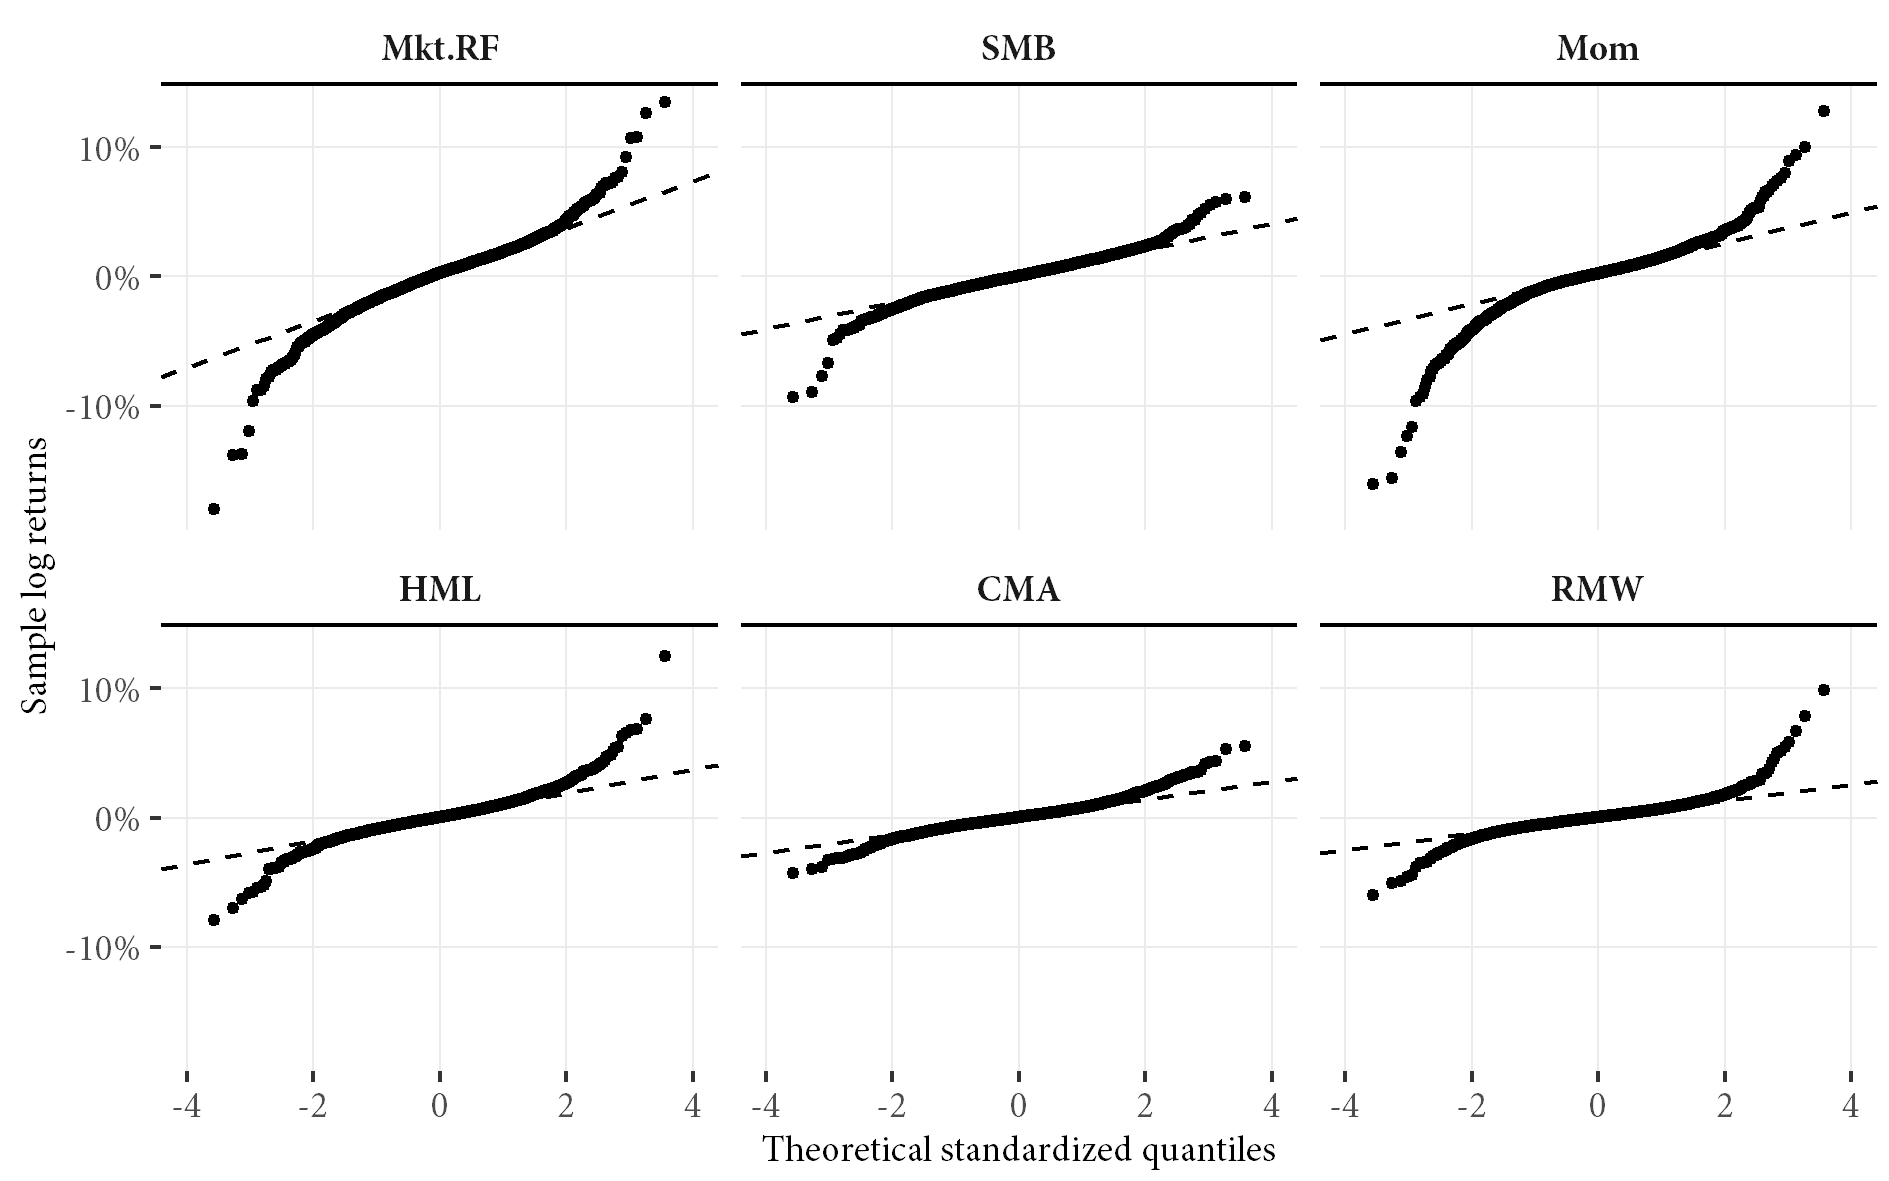
\includegraphics[scale=1]{graphics/qq_returns.png}  
  %\bottomrule
  \vspace{3mm}
  \footnotesize
  Quantile-quantile plots of theoretical (normal) and sample quantiles. Data from a normal distribution should line up on the dashed line. Weekly log returns 1963-2016
  \end{minipage}
\end{figure}


We conduct Ljung-Box tests of the factor returns to control for weekly autocorrelation.\footnote{For a detailed description of the test, see \autoref{sub:diagnostic_test_procedures}} The p-values of these tests are given in \autoref{tab:summarydata} and are very low for all factors except Mkt-RF, leading to a strong rejection of the zero autocorrelation null hypothesis. For Mkt-RF, the p-value is not enough for a rejection of zero autocorrelation at the 5 week maximum lag length, but strongly rejected for 10 weeks of maximum lags. We also conduct Ljung-Box tests of the squared factor returns to control for volatility clustering (ARCH effects). Here, the null hypothesis is that there are no ARCH effects, and p-values given in \autoref{tab:summarydata} strongly rejects the null for all factors at both max lag length of 5 and 10.

We conclude that factor return series are non-normal and exhibit both autocorrelation as well as autoregressive heteroscedasticity. These predictable phenomena in financial return data are typically captured by models that incorporate autoregressive components for both the conditional mean and variance equations, such as the family of ARMA-GARCH models, which are further discussed in \autoref{sec:univariate_modeling}.
\begin{figure}[H]
  \caption{Cumulative returns to factor strategies}
  \label{fig:cumret}
  %\toprule
  \centering
  \begin{minipage}{\textwidth}
  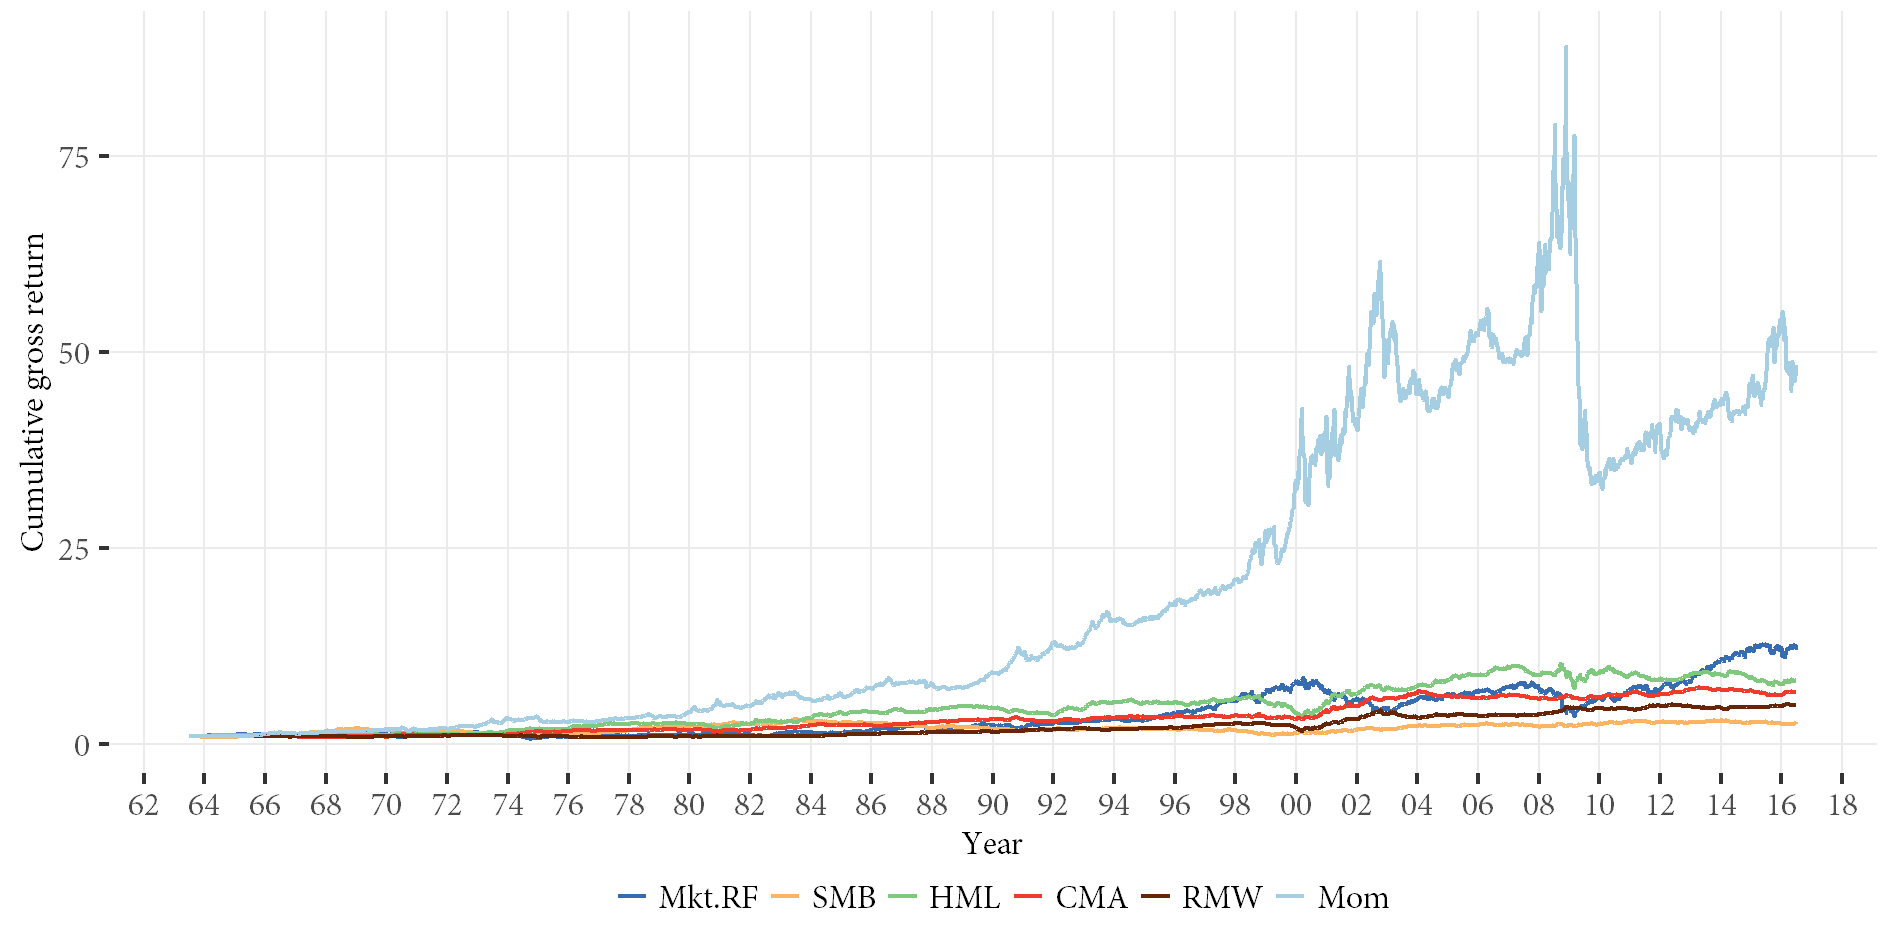
\includegraphics[scale=1]{graphics/cumretPlot.png}  
  %\bottomrule
  \vspace{3mm}
  \footnotesize
  Cumulative returns to investing one dollar in each factor strategy beginning 1963-07-05.  All data 1963-07-05 - 2016-07-01.
  \end{minipage}
\end{figure}
\begin{figure}[H]
  \caption{Standardized cumulative returns to factor strategies}
  \label{fig:cumretstd}
  %\toprule
  \centering
  \begin{minipage}{\textwidth}
  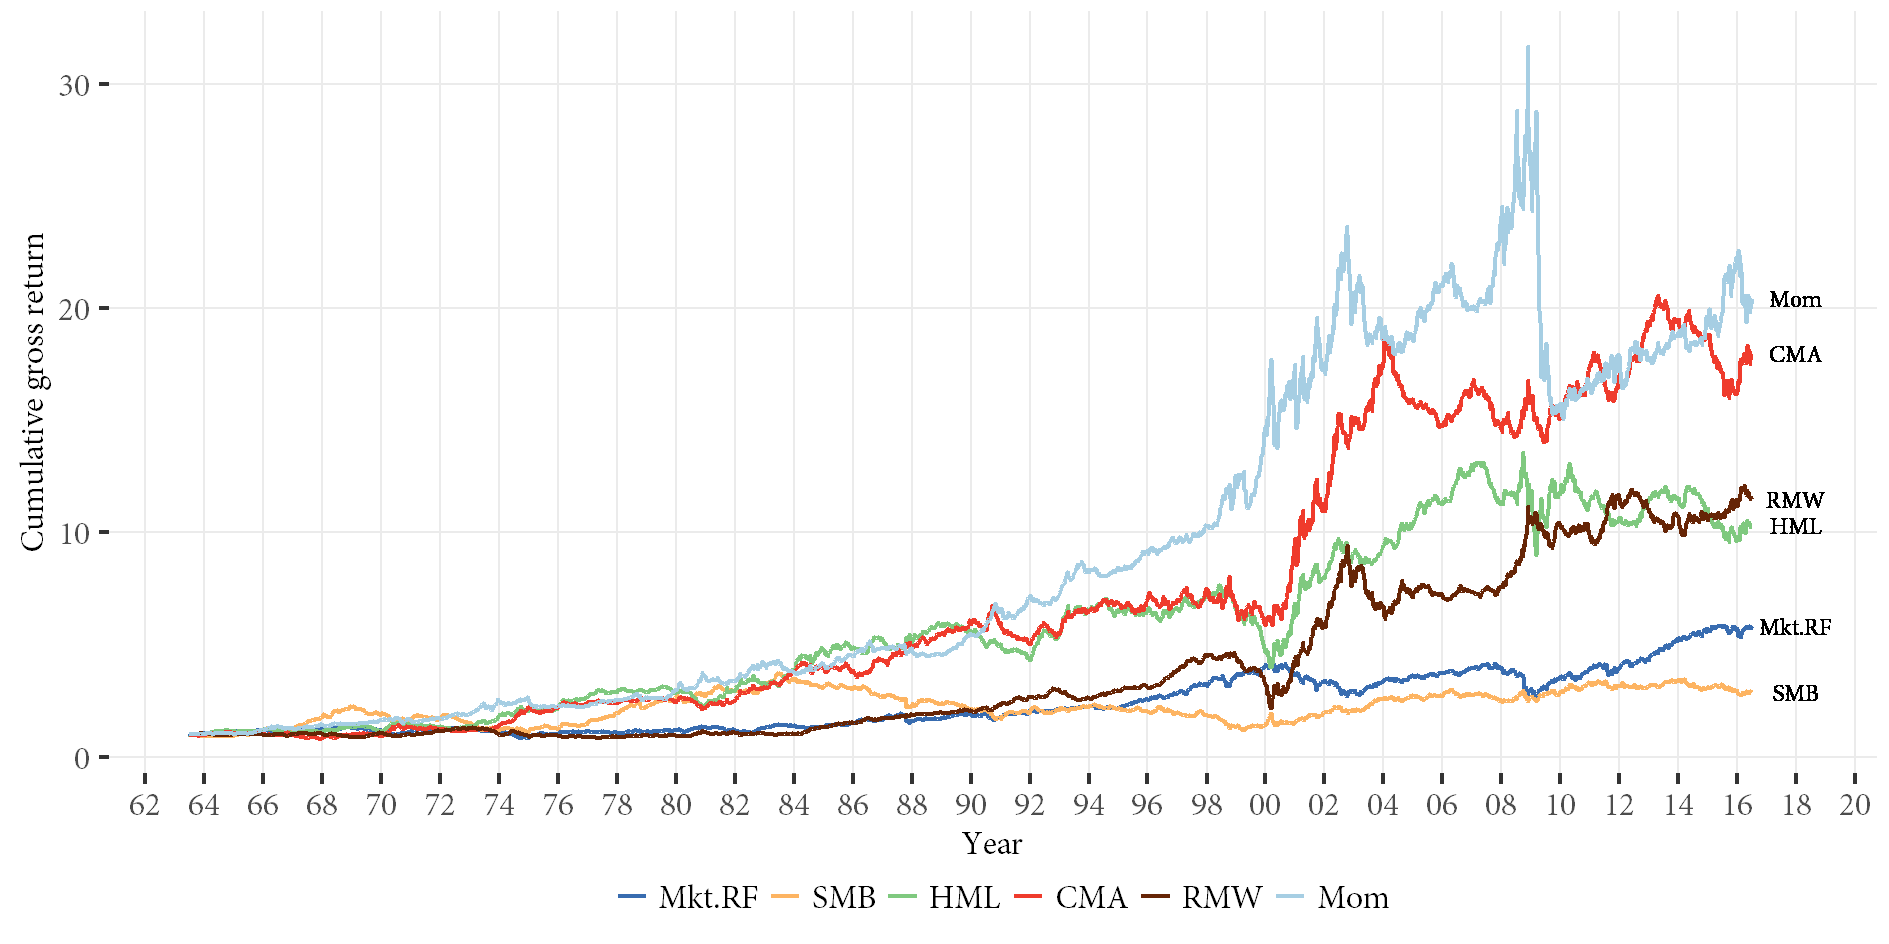
\includegraphics[scale=1]{graphics/cumretStdPlot.png}  
  %\bottomrule
  \vspace{3mm}
  \footnotesize
  Cumulative returns to investing one dollar in each factor strategy beginning 1963-07-05. Standardized to 10\% annual volatility. All data 1963-07-05 - 2016-07-01.
  \end{minipage}
\end{figure}

Plots of cumulative returns (\autoref{fig:cumret}) clearly show the high returns to the momentum strategy through the sample period. However, normalizing the series to 10\% annual volatility (\autoref{fig:cumretstd}) gives a more nuanced picture of mean-variance performance. Since 1963, each of the strategies except for SMB has outperformed the market factor. Furthermore, factor strategies seem to crash at different times and diversify eachother, e.g. Mom performing well during 1999-2000 and RMW performing well during 2008-2009. The unconditional correlation matrix of returns is given in \autoref{tab:corr_matrix} and the general low or even negative correlation coefficients show the diversification benefits of factor strategies. The HML - CMA pair does stand out, however, with an unconditional correlation of 0.625, which could be related to a partial overlap of the factor components as discussed in \autoref{sec:literature} -- past investment is shown to be positively empirically related to the current book-to-market ratio. The substantially higher correlation in this asset pair indicates lower diversification benefits between the two strategies and begs the question whether both should be included in a factor portfolio.

\begin{table}[!htbp] \centering 
  \caption{Correlation matrix} 
  \label{tab:corr_matrix} 
\begin{tabularx}{\textwidth}{X}
  \\[-1.8ex]%\toprule
  \\[-1.8ex] 
  \footnotesize Unconditional sample correlation matrix of factor log return series. Weekly data 1963-2016
\end{tabularx}
\begin{tabularx}{\textwidth}{@{\extracolsep{5pt}} X r r r r r r} 
  \\[-1.8ex]\midrule
  \\[-1.8ex] 
  & Mkt.RF & SMB & Mom & HML & CMA & RMW \\ 
\hline \\[-1.8ex] 
Mkt.RF & $1.000$ & $$ & $$ & $$ & $$ & $$ \\ 
SMB & $0.086$ & $1.000$ & $$ & $$ & $$ & $$ \\ 
Mom & $$-$0.113$ & $$-$0.007$ & $1.000$ & $$ & $$ & $$ \\ 
HML & $$-$0.283$ & $$-$0.026$ & $$-$0.219$ & $1.000$ & $$ & $$ \\ 
CMA & $$-$0.416$ & $$-$0.048$ & $0.071$ & $0.625$ & $1.000$ & $$ \\ 
RMW & $$-$0.154$ & $$-$0.337$ & $0.080$ & $$-$0.054$ & $$-$0.067$ & $1.000$ \\ 
%\bottomrule \\[-1.8ex] 
\end{tabularx} 
\end{table}
%!TEX root = ../main.tex

\section{Zero-cost portfolio regressions}
\label{sec:alpha_reg}
\textcite{FF2015} and \textcite{Asness2015} run factor regressions where both the LHS variable and the RHS variables are zero-cost factor portfolios. The intercept in these regressions is to be interpreted as the abnormal return, or Jensen's alpha, of adding the LHS factor to a portfolio already consisting of the RHS factors \autocite{Jensen1968}. In this section, we replicate and discuss the regressions where HML, CMA and RMW are the LHS variables, and find that previous results hold up in our weekly data set.

\subsection{Regression Models}

As a specific example, we begin by considering the regression that has caused the discussion on whether HML is a redundant variable. \textcite{FF2015} run the regression
\begin{align}
  r^{HML}_t = \alpha + \beta_1 r^{Mkt.RF}_t + \beta_2 r^{SMB}_t + \beta_3 r^{RMW}_t + \beta_4 r^{CMA}_t + \epsilon_t
\end{align}
where $r^i_t$ denote monthly returns. The central finding is that HML is completely subsumed by the four factors Mkt.RF, SMB, RMW and CMA -- the alpha of the regression is very small and not statistically significant. In other words, adding HML to a portfolio of the other four factors should give no alpha.

Our regression analysis deviates from that in \textcite{FF2015} as we consider weekly return data and a slightly extended data window. However, the main regression specifications are the same. We also consider a six-factor model, as done by \textcite{Asness2015}, who show that there is in fact added value of HML when momentum is included in the regression. We use standard errors that are adjusted for serial correlation found in the return data.

\subsection{Regression Results}

In \autoref{fig:abnormal}, regressions for the five-factor and six-factor models are presented. Each column represents one unique regression, with one of the factors as the LHS variable and with the remaining four (or five) factors as RHS variables (in rows).

First, we examine regression (1) in a five-factor model where HML is the LHS variable. We note that the alpha of HML is not significant, indicating that the factor is completely subsumed by the remaining four factors and does not create additional value in a portfolio setting, in line with~\textcite{FF2015}. More specifically, the only factor that explains HML is CMA, with a high coefficient of 0.85, with all other factor loadings insignificant and close to zero. Put differently, this suggests that for a factor portfolio already loaded on Market, CMA, SMB and RMW adding HML will load up additionally on CMA risk plus the idiosyncratic risks of HML without any additional return.

Second, we turn to regression (2) in a five factor model where CMA is the LHS variable. Here, the alpha is significant, indicating that the factor does provide an additional 0.06\% weekly beyond the existing four factors. While the CMA factor loads positively 0.39 on HML, this is substantially lower than HML's loading on CMA of 0.85. Put differently, CMA seems to be load on other factors than HML to a higher extent than vice versa. With CMA as the LHS variable, there is a significant negative loading on Mkt-RF, a significant negative loading on RMW and a significant positive loading on Mom. The CMA portfolio loads relatively less on the market, relatively more on unprofitable stocks (negative RMW) and loads relatively more on stocks with high recent returns (positive Mom) than does HML.

Third, we study regression (3) where RMW is the LHS variable. The alpha is significant, indicating that the RMW factor adds abnormal return of 0.09\% weekly to the four existing factors. In terms of factor loadings, profitability loads zero or negatively on all four remaining factors in the five-factor model. Especially noteworthy are the large negative loadings on SMB and CMA of -0.24 and -0.15, which suggests that SMB is comprised relatively more of large firms and investing firms. The fact that there are only negative loadings is in itself evidence of the great diversification that RMW provides -- it even covaries negatively with all five factors. The low explanatory power of the other factors is summarized by a low 15\% r-squared.

%!TEX root = ../../main.tex

\begin{table}
  \centering
  \footnotesize
  \renewcommand{\arraystretch}{1.2}

  \caption{Zero-cost portfolio regressions (1963--2016)}

  \begin{longcaption}
    Six regressions of zero-cost equity factor portfolios on $N = 2766$ weekly returns 1963--2016, following the analysis of~\textcite{FF2015} and~\textcite{Asness2015}. Alpha and Beta (factor loadings) of the column's portfolio on other factors. Heteroskedacity and autocorrelation robust standard errors in parentheses, following~\textcite{NeweyWest1987}. Significance given by $^{*}p<10\%$; $^{**}p<5\%$; $^{***}p<1\%$
  \end{longcaption}
  \label{fig:abnormal} 
\begin{tabularx}{\textwidth}{@{\extracolsep{0pt}}X d d d d d d d } 
\toprule
& \multicolumn{3}{c}{Five Factors} & & \multicolumn{3}{c}{Six Factors} \\ 
\cmidrule{2-4} \cmidrule{6-8}
 & \multicolumn{1}{c}{(1)} & \multicolumn{1}{c}{(2)} & \multicolumn{1}{c}{(3)}   & & \multicolumn{1}{c}{(4)} & \multicolumn{1}{c}{(5)} & \multicolumn{1}{c}{(6)} \\
 & \multicolumn{1}{c}{HML} & \multicolumn{1}{c}{CMA} & \multicolumn{1}{c}{RMW}   & & \multicolumn{1}{c}{HML} & \multicolumn{1}{c}{CMA} & \multicolumn{1}{c}{RMW} \\
\midrule \\ 
 \text{Alpha (\%)} & 0.02       & 0.06^{***}  & 0.09^{***}  & & 0.05^{**}   & 0.04^{***}  & 0.09^{***} \\
                   & (0.02)     & (0.01)      & (0.02)      & & (0.02)      & (0.01)      & (0.02) \\
  \\
 \text{Mkt.RF}     & -0.02      & -0.11^{***} & -0.08^{***} & & -0.03       & -0.10^{***} & -0.07^{***} \\
                   & (0.03)     & (0.02)      & (0.01)      & & (0.03)      & (0.01)      & (0.01) \\
  \\
 \text{SMB}        & 0.001      & -0.03       & -0.24^{***} & & 0.01        & -0.03^{*}   & -0.24^{***} \\
                   & (0.03)     & (0.02)      & (0.04)      & & (0.03)      & (0.02)      & (0.05) \\
  \\
 \text{HML}        &            & 0.39^{***}  & -0.01       & &             & 0.42^{***}  & 0.01 \\
                   &            & (0.04)      & (0.06)      & &             & (0.03)      & (0.06) \\
  \\
 \text{CMA}        & 0.85^{***} &             & -0.15^{**}  & & 0.87^{***}  &             & -0.17^{***} \\
                   & (0.04)     &             & (0.07)      & & (0.04)      &             & (0.06) \\
  \\
 \text{RMW}        & -0.02      & -0.09^{**}  &             & & 0.01        & -0.10^{**}  & \\
                   & (0.09)     & (0.04)      &             & & (0.07)      & (0.04)      & \\
  \\
 \text{Mom}        &            &             &             & & -0.18^{***} & 0.09^{***}  & 0.03 \\
                   &            &             &             & & (0.04)      & (0.02)      & (0.03) \\
\midrule
$R^2$ (\%) &
  \multicolumn{1}{D{.}{.}{2}}{39} &
  \multicolumn{1}{D{.}{.}{2}}{46} &
  \multicolumn{1}{D{.}{.}{2}}{15} & &
  \multicolumn{1}{D{.}{.}{2}}{47} &
  \multicolumn{1}{D{.}{.}{2}}{49} &
  \multicolumn{1}{D{.}{.}{2}}{15} \\ 
\bottomrule
\end{tabularx} 
\end{table}


Now, we move to the six-factor regression results, where we include the momentum factor Mom. First, in regression (4) with HML as the LHS variable, we note that the addition of HML has made the alpha of HML positive and significant -- in line with~\textcite{Asness2015}. As momentum is correlated with both the LHS and RHS factors, it constituted an omitted variable bias on the beta factor loadings in the five-factor model. HML has a substantial negative loading on the Mom factor of -0.18, while the CMA regression instead has a positive Mom loading of 0.09, suggesting that the seemingly similar factors are quite different in terms of momentum properties. HML firms are generally comprised of recent losers, while CMA firms are recent winners. The momentum factor has explained an additional 8\% of the variance in the HML factor.

As in the five-factor model, we also note differences in some of the other factor loadings between HML and CMA in the six-factor model. The CMA regression (reg. 5) loads relatively less on the market and relatively more on unprofitable stocks. It therefore seems that while HML and CMA firms share certain properties, HML firms are generally more profitable and less comparable to holding the market itself. The profitability factor (reg. 6) is largely unaffected by the addition of momentum the six-factor specification, which is expected given the low correlation (0.08) between the RMW and Mom factors. 

Although we employ weekly data, our results are qualitatively similar to the results in \textcite{FF2015} as well as in \textcite{Asness2015}. The alpha of HML is only recognized in a model including momentum. This finding indicates that the insignificant alpha of HML in the five-factor model might be due to the omission of an important control variable, momentum, that is included in the six-factor-model. This does suggest that HML is not dead, when including momentum.



%!TEX root = ../main.tex

\section{Modeling of factor returns} % (fold)
\label{sec:modeling_of_factor_returns}

% Why a model?
This section presents our model for the joint behavior of returns. A multivariate model of returns allows us to make conditional forecasts of the distribution of returns one week ahead, which take into account the dependence between factors. The model is used in the mean-variance analysis, to provide dynamic inputs that can give us optimal weights over time. The model is also used in the analysis of diversification benefits, when we shift the focus to the tail risk of factor portfolios. First, we describe why we choose the copula model among different multivariate models. Second, we define the model and interpret the parameterization. Third, we select and estimate univariate models that are building blocks in the copula. Fourth, we analyze residuals from univariate models, to determine what type of multivariate dependence the copula should capture. Fifth, we estimate the copula and choose the best specification. Last, we conduct a robustness check of whether the copula captures the dependence structure.

%!TEX root = ../main.tex

\subsection{Choosing a multivariate model}
\label{sub:05_01_choosing}
% Why copula?
The ARMA-GARCH family of models has become the norm of modeling univariate financial return series, beginning with \textcite{Bollerslev1986}. The straightforward extension of univariate GARCH models to multiple return series has, however, proven difficult. Unrestricted multivariate GARCH (MGARCH) models that model the conditional covariance matrix directly become impossible to estimate as the number of covariances grows exponentially with the number of series. It thus becomes necessary to restrict the parameter space, where the BEKK model is a common example~\autocite{BEKKModel}.

% Separate modeling of variance and correlation
A parsimonious solution to the dimensionality problem is to separate the modeling of return and volatility dynamics from the modeling of conditional correlations. The separation allows for consistent (albeit inefficient) two-step estimation, and makes large-scale estimation feasible. One such approach is the \emph{dynamic conditional correlation} (DCC) model originally proposed by~\autocite{Engle2002}. In the DCC model, univariate GARCH models are first estimated on each series. Then, an autoregressive process for the correlation matrix is fitted to the standardized residuals ${z_t}$ of those models. 

% Asymmetric cDCC and copula cDCC
DCC is a useful and tractable model for estimating time-varying correlations between return series. However, it is a model of correlations only; it is not flexible enough to model the univariate components differently. More specifically, it is not constructed to generate tail dependence, which is the notion that correlation dynamics can be very different in extreme realizations. 

% Enter the copula
Copula models have recently attracted much attention in the field of risk management, as they provide a flexible way to infer a multivariate probability distribution. Copula models are, just like DCC models, based on two-step estimation and work well in large scale applications. Furthermore, copulas are flexible enough to generate tail dependence, which is shown to be an important feature of factor return data~\autocite{ChristoffersenLanglois2013}. 

Copula models are most often constructed by estimating univariate models from the ARMA-GARCH family in the first step. The residuals from the ARMA-GARCH models are then used in the copula function that explains the multivariate dependence, including dynamic correlations and tail dependence.

Among copula models, there are three main routes of interest: (1) Archimedean copulas, (2) multivariate normal and Student's \textit{t} copulas, and (3) vine copulas. While Archimedean copulas, such as the Gumbel and Clayton specifications, are attractive in many settings, they fail to generate both threshold correlations and simultaneously high unconditional correlations, and are hard to generalize beyond the bivariate case -- making them less attractive for factor return series \textcite{ChristoffersenLanglois2013}. Vine copulas, or pairwise copula constructions, are made up of a combination of bivariate copulas in a tree structure (hence the name vine copulas), and pose an interesting alternative to multivariate normal and Student's \textit{t} copulas. However, the vine method is far less parsimonious as both the number of bivariate combinations and the number of different tree structures increase exponentially with the number of assets modeled \autocite{Aas2009}.

We choose to work with multivariate Student's \textit{t} copula models, as they can (1) estimate the joint distribution function in large scale applications, (2) model different univariate models for the different factors, and (3) incorporate both tail dependence and dynamic correlations. Next, we define and describe the copula model. % motivating the choice of copula, and among copulas

%!TEX root = ../../main.tex

\subsection{Definition of copula model} % (fold)
\label{sub:definition_of_copula_model}

Each week $t$, the conditional joint density of returns on $N$ assets $R_{t+1} = \{r_{i,t+1},\ldots,r_{N,t+1}\}$ is described by a joint density function $f_t(R_{t+1})$. Following~\textcite{ChristoffersenErrunzaJacobLanglois2012}, who build on~\textcite{Patton2006} and~\textcite{Sklar1959}, we decompose the joint density function into the product of a joint copula function $c_t(U_{t+1})$ of uniformly distributed variables $U_{t+1} \sim U(0, 1)$ and marginal densities $f_{i,t}(r_{i,t+1})$:
\begin{align}
  f_t(R_{t+1}) =
    c_t(U_{t+1}) \prod^N_{i=1} f_{i,t}(r_{i,t+1})
  \label{eq:copula_sklar}
\end{align}
The elements of $U_{t+1} = \{u_{i,t+1},\ldots,u_{N,t+1}\}$ are related to the original returns by the probability integral transform, i.e the cumulative distribution of $r_{i,t+1}$:
\begin{align}
  u_{i,t+1} = F_{i,t}(r_{i,t+1}) = \int_{-\infty}^{r_{i,t+1}} f_{i,t}(r)dr
\end{align}
The copula function $c_t(U_{t+1})$ is a multivariate skewed \emph{t} distribution. This distribution is parameterized by a single degrees of freedom parameter $\nu_c$, controlling the degree of dependence, a vector of $N$ skewness parameters $\gamma_c$, controlling the asymmetry in dependence, and a potentially time-varying correlation matrix $\Psi_{t}$.\footnote{We describe the details of the skewed \emph{t} distribution, including the expanded form of $c_t$, in~\autoref{app:ghstmv}.} The skewed \emph{t} distribution nests the standard (hereafter symmetric) \emph{t} distribution when all $\gamma_{i,c} = 0$ and the standard normal distribution when additionally $\nu_c = \infty$.

The log-likelihood of the model is constructed from~\autoref{eq:copula_sklar}:
\begin{align}
  L =
    \underbrace{\sum_{t=1}^T \log(c_t(U_{t+1}))}_\text{Copula} +
    \underbrace{\sum_{t=1}^T \sum_{i=1}^N \log(f_{i,t}(r_{i,t+1}))}_\text{Marginals}
\end{align}
At this point, it is worth noting that the joint density $c_t(U_{t+1})$ need not be of the same family as the marginal densities $f_{i,t}(r_{i,t+1})$ -- nor are we restricted to modeling $f_{i,t}(r_{i,t+1})$ jointly for all factors. In fact, we take advantage of this flexibility and choose to model the marginal densities independently as ARMA-GARCH processes, which allows us to capture a number of predictable features in the univariate series -- serial correlation, volatility clustering and leverage effects. The marginal models are estimated independently by maximizing the likelihood(s) of the second term, and then the copula is estimated by maximizing the first term -- using the residuals of the marginal models as given.

This procedure is called multi-stage maximum log-likelihood or inference functions for margins and greatly simplifies the estimation procedure, while yielding relatively efficient estimates~\autocite{Patton2006,Joe1997}. The modeling and estimation of our ARMA-GARCH models is detailed in the upcoming subsection, whereas the remainder of this subsection describes how we make the correlation matrix $\Psi_t$, and thus the dependence between factors, dynamic.

The copula is made dynamic by fitting a dynamic conditional correlation (DCC) process for $\Psi_t$ to copula residuals $z_{t+1}^*$~\autocite{Engle2002}. Using the notation from~\textcite{ChristoffersenLanglois2013}:
\begin{align}
  Q_t = (1 - \alpha - \beta) Q
    + \beta Q_{t-1}
    + \alpha \bar{z}_{t-1}^* \bar{z}_{t-1}^{*\top}
  \label{eq:copula_cdcc}
\end{align}
where $Q_t$ is normalized to the correlation matrix $\Psi_t$:
\begin{align}
  \Psi_t = Q_t^{-\frac{1}{2}} Q_t Q_t^{-\frac{1}{2}}
  \label{eq:copula_cdcc_psi}
\end{align}
The $Q_t$ process is comprised of three components that are weighted according to $\alpha, \beta$: (1) a time-invariant component: $Q$, (2) an innovation component from copula shocks: $\bar{z}_{t-1}^{*} \bar{z}_{t-1}^{*\top},$\footnote{Where $\bar{z}_{i,t+1}^* = z_{i,t+1}^* \sqrt{q_{ii,t}}$ is due to a correction by~\textcite{Aielli2013}, that improves the reliability of the estimation procedure.} and (3) an autoregressive component of order one: $Q_{t-1}$. In order for the the correlation matrix $\Psi_t$ to be positive definite, $Q_t$ has to be positive definite, which is ascertained by requiring that $\alpha \geq 0$, $\beta \geq 0$ and $(\alpha + \beta) < 1$. The model nests a constant copula when $\alpha = \beta = 0$.

The model for $c_t(U_{t+1})$ is comprised of $1 + N$ distribution parameters $\{\nu_c, \gamma_c\}$ and $2 + \frac{N(N-1)}{2}$ dynamics parameters $\{\alpha, \beta, Q\}$, where the elements of $Q$ are estimated using moment matching, and the remaining parameters $\{\alpha, \beta, \nu_c, \gamma_c\}$ are estimated using maximum likelihood.\footnote{A detailed description of the copula estimation procedure can be found in~\autoref{app:copula_cdcc}.}

ARMA-GARCH modeling allows us to filter time-varying effects, leaving independent \emph{standardized residuals} $z_{i,t}$, which are assumed to follow a constant distribution $f_i(z_{i,t})$. These residuals are first transformed into uniform variables $u_{i,t+1}$ by the probability integral transform of the densities above, and then made to follow the \emph{copula} distribution by the \emph{inverse} probability integral transform of the \emph{copula}:
\begin{align}
  z_{i,t+1}^* = F^{-1}_{\nu_c,\gamma_{i,c}}(F_{i}(z_{i,t+1}))
\end{align}

The interpretation of the copula parameterization is closely associated to the structure of multivariate dependence. By different restrictions on the parameters in the DAC model, we are able to activate or deactivate certain features of the copula: First, the degree of freedom parameter $\nu_c$ is to be interpreted as the measure of tail dependency. When $\nu \neq 0$, the lower and upper tails of the joint distribution are fatter than in the normal case, which is coherent with earlier evidence of threshold correlations~\autocite{ChristoffersenLanglois2013}. Second, the skewness parameters $\gamma_{c,i}$ are to be interpreted as the extent of asymmetry in the correlation structure. When $\gamma \neq 0$, there is asymmetry in correlations. Third, the $\alpha$ and $\beta$ parameters determine whether the copula generates time-varying correlations. If $\alpha \neq 0$ and $\beta \neq 0$, the copula is dynamic. An overview of the six copula models is given in \autoref{tab:conceptual}.

%!TEX root=../../main.tex

\begin{table}
  \centering
  \footnotesize
  \renewcommand{\arraystretch}{1.2}

  \caption{Conceptual matrix of copula parameterizations}

  \begin{tabularx}{0.80\textwidth}{@{} lc c >{\centering}Xc >{\centering}Xc >{\centering\arraybackslash}X}
    \toprule
      & && \textbf{Normal} && \textbf{Symmetric \emph{t}} && \textbf{Skewed \emph{t}} \\
      \cmidrule{4-4}
      \cmidrule{6-6}
      \cmidrule{8-8}
      & && $\nu_c = \infty$   && $\nu_c < \infty$   && $\nu_c < \infty$ \\
      & && $\gamma_{i,c} = 0$ && $\gamma_{i,c} = 0$ && $\gamma_{i,c} \neq 0$ \\
      \cmidrule{4-8}
    \cmidrule{1-2}
    \multirow{2}{*}{\textbf{Constant}} & $\alpha = 0$ && Constant && Constant && Constant \\
                              & $\beta = 0$  && Normal   && Symmetric \emph{t} && Skewed \emph{t}      \\
    \cmidrule{1-2}
    \multirow{2}{*}{\textbf{Dynamic}}  & $\alpha > 0$ && Dynamic  && Dynamic && Dynamic \\
                              & $\beta > 0$  && Normal   && Symmetric \emph{t} && Skewed \emph{t}      \\
    \bottomrule
  \end{tabularx}
% ()
%   \begin{tabularx}{\textwidth}{@{\extracolsep{5pt}} c c c c X c X c @{}}
%     \toprule
%   				&			& &	\textbf{Normal}	&	&	\textbf{Student's \textit{t}}	&	&	\textbf{Asymmetric Student's \textit{t}} \\
%   				\\
%   				&			& & 	$\nu = \infty$	&	&	$\nu > 0$	& 	&	$\nu > 0$ \\
%   				&			& & 	$\gamma = 0$	&	&	$\gamma = 0$	& 	&	$\gamma \neq 0$ \\
%           \\
%     \cmidrule{4-8}
%     \\
%      \textbf{Constant} &  & & \text{Constant normal copula} & & \text{Constant symmetric \textit{t} copula} & & \text{Constant asymmetric \textit{t} copula} \\
%      \\
%     	&	$\alpha = 0$  &		&	\textit{Constant correlations but} & & \textit{Constant correlations and} & & \textit{Constant correlations and} \\
%        & $\beta = 0$ & & \textit{no tail dependence} & & \textit{symmetric tail dependence} & & \textit{asymmetric tail dependence} \\
%     \\
%     \cmidrule{4-8}
%     \\
%      \textbf{Dynamic} &  & & \text{Dynamic normal copula} & & \text{Dynamic symmetric \textit{t} copula} & & \text{Dynamic asymmetric \textit{t} copula} \\
%      \\
%       & $\alpha > 0$  &   & \textit{Dynamic correlations but} & & \textit{Dynamic correlations and} & & \textit{Dynamic correlations and} \\
%        & $\beta > 0$ & & \textit{no tail dependence} & & \textit{symmetric tail dependence} & & \textit{asymmetric tail dependence} \\
%     \\
%     \bottomrule
%   \end{tabularx}

  \label{tab:conceptual}	
\end{table}



% subsection definition_of_copula_model (end)
 % the boom

%!TEX root = ../../main.tex

\subsection{Univariate modeling of returns} % (fold)
\label{sub:univariate_modeling_of_returns}

We proceed by estimating models of each factor's return series, which attempt to capture predictable autocorrelation, volatility clustering and leverage effects. By fitting ARMA-GARCH models, we can filter these effects and reduce the time-varying densities $f_{i,t}(r_{i,t+1})$ to constant densities of \emph{standardized residuals} $f_{i}(z_{i,t+1})$.

\subsubsection{General univariate model: ARMA-GJR-GARCH}

The ARMA-GARCH is a broad model family designed to model predictable components of financial return series, and was originally introduced by~\textcite{Bollerslev1986}. The models use autoregressive and moving average lags to capture serial correlation in return data (ARMA), as well as autoregressive and moving average lags to capture ARCH effects in residuals from the mean equation (GARCH). We evaluate the GJR-GARCH model of~\textcite{glosten1993relation}, which is a parsimonious extension of the standard GARCH(1, 1). The GJR-GARCH is designed to also capture leverage effects~\autocite{glosten1993relation}, i.e. when positive and negative return shocks have different impact on future volatility~\autocite{Black1976}.

We estimate conditional mean equations for each factor \emph{up to} ARMA(3, 3):
\begin{align}
  r_{i,t} &=
    \phi_{i,0} +
    \sum^p \phi_{i,p} r_{i,t - p} +
    \sum^q \theta_{i,q} \varepsilon_{i,t - q} + 
    \varepsilon_{i,t}
    \label{eq:garch_mean}
\end{align}
where $r_{i,t}$ are weekly returns of each factor. The conditional volatility evolves according to the GJR-GARCH specification:
\begin{align}
  \varepsilon_{i,t} &= \sigma_{i,t} z_{i,t} \\
  \sigma_{i,t}^2 &=
    \omega_i +
    (\alpha_i + \eta_i I_{\varepsilon_{i,t-1} \leq 0}) \varepsilon_{i,t - 1}^2 +
    \beta_{i} \sigma^2_{i,t - 1}
    \label{eq:garch_garch}
\end{align}
where $I$ is an indicator function that is equal to one when $\varepsilon_{i,t-1} \leq 0$. 

A positive $\eta_i$ captures the leverage effect by increasing the current period's volatility if the previous period's residual $\varepsilon_{i,t-1}$ was below zero. A significant $\eta_i$ thus introduces asymmetric volatility in the model. For the market factor, it is expected that $\eta_i$ is positive, reflecting the leverage effect in the market itself, and no impact from the short risk-free component. However, for the other factors, which are constructed as all-equity zero-cost long-short portfolios, the direction of $\eta_i$ is less obvious~\autocite{ChristoffersenLanglois2013}. If there are leverage effects for stocks in general, negative shocks will lead to more volatility than positive shocks in a portfolio of stocks. But in a zero-cost portfolio, the leverage effects of the long positions in stocks could be offset by the short positions in other firms. The level of the leverage effect in a zero-cost portfolio therefore depends on the relative strength of leverage effects in the long and short components.

% XXX In the estimation, we also use variance targeting as proposed by~\textcite{EngleMezrich1995}, which is shown makes optimization faster and sometimes more certain to reach the global maximum. This means that $\omega$ is not estimated in the maximum likelihood setting, but instead set to 1 minus the persistence of the process times the sample mean of squared residuals, where the persistence is $\alpha + \beta$ for the GARCH.\footnote{Note that in the case of the GJR-GARCH for the Mkt.RF factor, the persistence is $\alpha + \beta + \eta \kappa$ where $\kappa$ is the probability that standardized residuals $z_t$ are below zero.}
The ARMA-GARCH models are estimated independently on each series using maximum likelihood estimation, with assumed distributions of standardized residuals $z_{i,t}$. Similar to the multivariate copula, we evaluate models where the standardized residuals are assumed to follow univariate skewed \emph{t} distributions with $\nu_i$ degrees of freedom and skewness $\gamma_i$, nesting the symmetric \emph{t} when $\gamma_i = 0$ and the standard normal when $\nu_i = \infty$. A skewed \emph{t} distribution allows for additional asymmetry beyond the GJR-GARCH leverage effect~\autocite{ChristoffersenErrunzaJacobLanglois2012}.

\subsubsection{Factor specific model selection process}

Our selection process is as follows.

\begin{enumerate}[(i)]
  \item For each factor strategy, we estimate GJR-GARCH models on the full dataset ($T = 2,766$) up to~ARMA(3,~3) and~GARCH(1,~1) under normal, symmetric \emph{t} and skewed \emph{t} residuals, with and without $\eta_i$ fixed to zero (in which case we obtain the basic~GARCH(1,~1) model).
  \item We then compute the Bayesian Information Criterion~\autocite[BIC]{Schwarz1978} for each factor strategy and specification and select the ARMA order with the lowest BIC as our primary candidates.
\end{enumerate}

\noindent For the candidate models

\begin{enumerate}[(i)]
  \item We check for remaining serial correlation and ARCH effects using weighted portmanteau tests.
  \item We examine whether a sign bias test concludes that there are significant leverage effects that warrant the use of a GJR-GARCH instead of a standard GARCH.
  \item We use QQ-plots to control for misspecification in the residual process, and to find a suitable distribution for the standardized residuals $z_t$.
\end{enumerate}

In a well-specified model, we expect there to be no significant serial correlation, ARCH effects or leverage effects in the residuals. We employ weighted Ljung-Box, ARCH LM and sign bias tests that are detailed in \autoref{app:univariate_diagnostics}. Furthermore, the QQ-plots of the standardized residuals should show that their empirical distribution is comparable to the assumed theoretical distribution (i.e. be distributed around the 45 degree line).

\subsubsection{Model selection and estimation results}

The result of our selection and estimation procedure are presented in~\autoref{tab:garch_estimation}. The Mkt.RF factor is the only model that requires a GJR-GARCH $(\eta_i \neq 0)$, while the remaining models are all standard GARCH(1, 1). The minimization of BIC leads to ARMA(0, 0) for Mkt.RF, ARMA(1, 0) for CMA and Mom, and ARMA(1, 1) for the remaining factors SMB, HML and RMW. 



\begin{table}[!ht]
  \centering
  \scriptsize
  \renewcommand{\arraystretch}{1.2}

  \caption{Parameter estimates from ARMA-GARCH models in~\autoref{eq:garch_mean}and \autoref{eq:garch_garch} of weekly returns.\\ \quad \\
  Heteroskedasticity robust standard errors in parentheses, following \textcite{White1982}. Sample: 1963-07-05--2016-07-01 (2766 weekly obs). $\gamma$ and $\nu$ are the skewness and degree of freedom parameters of the skewed Student's \textit{t} innovations. $\eta$ is fixed at zero, as the sign bias test showed no significant misspecification of the GARCH for the HML, RMW and CMA factors. $\omega$ is set using variance targeting, following \textcite{EngleMezrich1995}. \emph{UV} is the estimate of unconditional volatility; \emph{VP} is the estimate of variance persistence. Ljung-Box and ARCH-LM tests are the weighted portmanteau tests from \textcite{FisherGallagher2012} and the sign bias test is from \textcite{EngleNg1993}, see appendix for details. Note: $^{*}$p$<$0.1; $^{**}$p$<$0.05; $^{***}$p$<$0.01}
  \begin{tabularx}{\textwidth}{@{}l X dddddd @{}}
    \toprule
    &&
      \multicolumn{1}{c}{Mkt.RF} &
      \multicolumn{1}{c}{SMB} &
      \multicolumn{1}{c}{Mom} &
      \multicolumn{1}{c}{HML} &
      \multicolumn{1}{c}{CMA} &
      \multicolumn{1}{c}{RMW} \\
    \midrule
    $\mu$ (\%) && 0.115^{***} & 0.032 & 0.137^{***} & 0.064^{**} & 0.040^{***} & 0.055^{***} \\
               && (0.031) & (0.032) & (0.046)& (0.025) & (0.012) & (0.016) \\
               \\
    $\phi_1$   &&         & 0.773^{***} & 0.129^{***} & 0.723^{***} & 0.111^{***} & 0.589^{***}\\
               &&         & (0.045) & (0.049) & (0.081) & (0.020) & (0.190) \\
               \\
    $\theta_1$ &&         & -0.651^{***} &      &   -0.610^{***} & & -0.466^{**} \\
               &&         & (0.056) &     &    (0.090)  & & (0.210) \\
               \\
    $\alpha$   && 0.032^{**} & 0.114^{***} & 0.183^{***} & 0.109^{***} & 0.088^{***} & 0.077^{***} \\
               && (0.014) & (0.023) & (0.008) & (0.002) & (0.002) & (0.002) \\
               \\
    $\beta$    && 0.845^{***} & 0.842^{***} & 0.796^{***} & 0.873^{***} & 0.899^{***} & 0.915^{***} \\
               && (0.007) & (0.035) & (0.009) & (0.002) & (0.001) & (0.001) \\
               \\
    $\eta$     && 0.189^{***} &  & \\
               && (0.024) &  & & \\
               \\
    $\gamma$   && -2.356^{**} & -0.650 & -2.124 & 0.627 & 0.484 & 0.248 \\
               && (0.836) & (1.036) & (9.898) & (0.405) & (0.493) & (0.421) \\
               \\
    $\nu$      && 13.246^{***} & 11.564 & 13.356 & 10.197^{***} & 11.094^{***} & 10.949^{*}\\
               && (3.505) & (12.085) & (40.035) & (2.669) & (3.481) & (5.652) \\
               \\
    $\omega\,\,(\text{permil}) $   && 0.016 & 0.006 & 0.007 & 0.003 & 0.001 & 0.001 \\
               && \\
    \midrule
    LLH  && \multicolumn{1}{r}{7,051} & \multicolumn{1}{r}{8,567} & \multicolumn{1}{r}{7,941} & \multicolumn{1}{r}{8,788} & \multicolumn{1}{r}{9,574} & \multicolumn{1}{r}{9,872} \\
    UV   && 0.022 & 0.010 & 0.017 & 0.010 & 0.010 & 0.010 \\
    VP   && 0.968 & 0.957 & 0.979 & 0.982 & 0.987 & 0.992 \\
    \midrule
    \multicolumn{8}{@{}l}{\textbf{p-values of Ljung-Box (LB), ARCH-LM and Sign Bias tests}} \\
    LB(5)          && 0.148 & 0.271 & 0.828 & 1.000 & 0.182 & 1.000 \\
    LB(10)         && 0.098 & 0.720 & 0.721 & 0.977 & 0.070 & 0.055 \\
    ARCH-LM(5)     && 0.812 & 0.626 & 0.053 & 0.117 & 0.837 & 0.724 \\
    ARCH-LM(10)    && 0.931 & 0.882 & 0.134 & 0.391 & 0.945 & 0.911 \\
    Sign bias [-]  && 0.883 & 0.331 & 0.836 & 0.094 & 0.473 & 0.204 \\
    Sign bias [+]  && 0.156 & 0.094 & 0.381 & 0.399 & 0.069 & 0.648 \\
    \bottomrule
  \end{tabularx}

  \label{tab:garch_estimation}
\end{table}


Based on these ARMA-GARCH specifications, the Ljung-Box and LM tests indicate no remaining serial correlation or ARCH effects at a 5\% significance level.

The lack of significant sign bias in the GARCH specifications for all models except Mkt.RF is interesting, and in line with the argument that any leverage effects could cancel out in a zero-cost long-short equity portfolio; the Mkt.RF is the only factor that is net-long equities and also exhibited leverage effects, with a negative sign bias as a GARCH model. We note that the sign bias of Mkt.RF has been eliminated in the GJR-GARCH model.

The candidate specifications under normal and symmetric \emph{t} distributed innovations all display misaligned QQ-plots (see~\autoref{fig:garch_qq}). The empirical distributions deviate from the 45 degree theoretical lines, especially in the more extreme quantiles. This indicates asymmetry in the residual series. In unreported results, we have controlled that the misspecification of normal and symmetric \emph{t} residuals is present even if GJR-GARCH models are fitted for all factors -- i.e. leverage effects cannot explain the misspecification. By comparison, the QQ-plots with skewed \emph{t} innovations seem to fit the data well. We proceed with skewed \textit{t} residual distributions.

\begin{figure}[!pt]
  \centering
  \footnotesize

  \begin{subfigure}{9cm}
    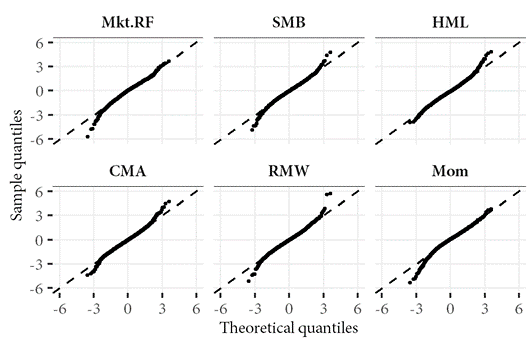
\includegraphics[width = 9cm]{graphics/qq_norm.png}
    \caption{Normal}
  \end{subfigure}
  \\
  \begin{subfigure}{9cm}
    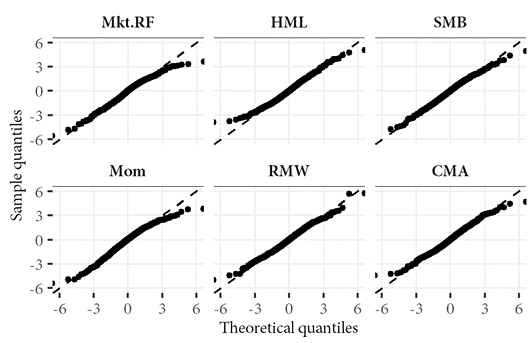
\includegraphics[width = 9cm]{graphics/qq_std.png}
    \caption{Symmetric \emph{t}}
  \end{subfigure}
  \\
  \begin{subfigure}{9cm}
    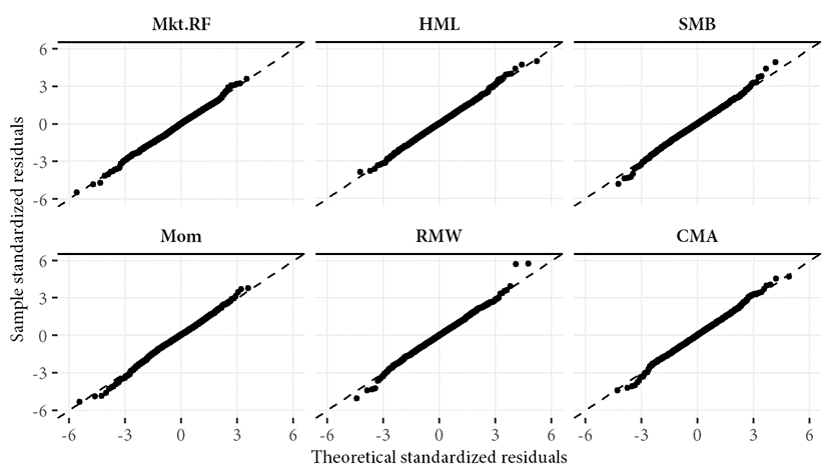
\includegraphics[width = 9cm]{graphics/qq_ghst.png}
    \caption{Skewed \emph{t}}
  \end{subfigure}
  \caption{QQ plots of standardized residuals}
  \begin{longcaption}
    Standardized residuals from the best (lowest BIC) ARMA-GARCH model specifications, with normal, symmetric \emph{t} and skewed \emph{t} innovations. Data from the theoretical distribution should line up on the dashed line. Based on weekly data 1963--2016.
  \end{longcaption}
  \label{fig:garch_qq}
\end{figure}

% In the variance equation, all factors exhibit high $\alpha$ and $\beta$ leading to a high variance persistence, between 0.96 and 0.99. Generally, variance persistence, which is related to volatility clustering, tends to be high in financial return series. [WHAT DOES IT MEAN WHY DO I CARE] We note that the zero-cost factor portfolios are no exception. The HML factor has a higher $\alpha$ estimate, indicating that shocks of equal size translate into slightly stronger volatility for HML than for RMW and CMA. RMW, on the other hand, has both the lowest $\alpha$ estimate and the highest $\beta$ estimate, indicating higher persistence and lower sensitivity of volatility to shocks.

% We note that the Mkt.RF factor is, according to our model selection procedure, best fitted by a ARMA(0, 0) mean equation, indicating no predictive power of 1-week lagged returns. Also, in the variance equation, we note that the relatively low $\alpha = 0.037$ sensitivity to shocks is increased considerably by $\eta = 0.181$ in the case of a \emph{negative} shock. Furthermore, the Mom factor stands out with a much higher estimate of $\alpha$ (0.186) than any of the other series (all around 0.10) and a lower $\beta$ (0.793). This means that volatility in the momentum factor is more sensitive than other factor strategies to return shocks and less predictable by past volatility alone. We also note that the Mkt.RF and Mom factors exhibit relatively higher unconditional volatilities (of 0.022 and 0.018) than do other factors (around 0.010).

Many of the estimates of $\gamma_i$, the skewness of the skewed \emph{t} GARCH innovation process, are statistically insignificant. This is also the case for the degree of freedom estimates, $\nu$ for the SMB and Mom models. Although these parameters are not significantly estimated, we believe that including them is essential, as QQ-plots indicate misspecification for the models with normal and symmetric \emph{t} innovations.

% subsection univariate_modeling_of_returns (end)
 % arma garch

%!TEX root = ../../main.tex

\subsection{Multivariate dependence} % (fold)

In this subsection, we demonstrate that the standardized residuals $z_{i,t}$ in our chosen ARMA-GARCH models display both asymmetric and time-varying dependence, shown by threshold and rolling correlations. ARMA-GARCH filtering has little effect on the (time-varying) correlations between factors. However, the use of the skewed \emph{t} distribution does remove a degree of asymmetry in the dependence. These patterns in multivariate dependence are the motivating reasons for a copula model, as they suggest that factor returns are not independent of each other after filtering for univariate effects, and that this dependence is not well-approximated by a normal model.\footnote{A visual comparison of dependence measures on returns compared to standardized residuals can be found in~\autoref{app:supplementary}.}

% XXX Här finns en liten karamell att suga på; gammal text nedan

% , measured by threshold correlations, and time-varying correlations, measured by rolling correlations, features we will attempt to model in the copula model. In the context of modeling, we are interested in the standardized residuals, rather than the returns themselves, as they are filtered of the variance dynamics present in the returns themselves~\autocite{ChristoffersenLanglois2013}.\footnote{The visual patterns for both threshold and rolling correlations are quite similar between returns and standardized residuals; results are available in the appendix.}

\subsubsection{Threshold correlations}

Threshold (or exceedance) correlations have previously been used to highlight the asymmetric dependence structure of i.a. country equity indices~\autocite{LonginSolnik2001}, portfolios by industry, size, value and momentum~\autocite{AngChen2002} and factor strategies~\autocite{ChristoffersenLanglois2013}. The following analysis is still new as it adds the investment (CMA) and profitability (RMW) factors. We follow~\textcite{ChristoffersenLanglois2013} definition of threshold correlation:
\begin{align}
\label{eq:th_corr}
    ThCorr(r_i, r_j) = 
    \begin{cases} 
        Corr\Big(r_i, r_j \,|\, r_i < F_i^{-1}(p), r_j < F_j^{-1}(p)\Big)  & \text{for } p < 0.5 \\
        Corr\Big(r_i, r_j \,|\, r_i \geq F_i^{-1}(p), r_j \geq F_j^{-1}(p)\Big)  & \text{for } p \geq 0.5
    \end{cases}
\end{align}
% XXX Be consistent with percentile and quantile
where $F_i^{-1}(p)$ is the empirical quantile of $r_i$ at percentile $p$. Threshold correlations thus reflect how series correlate when both are simulataneously realizing in their respective tails. This subsetting of data is illustrated in \autoref{fig:illustrate_threshold}. In the left hand plots, we see the scatter of ARMA-GARCH residuals of Mkt.RF and HML respectively, and how the threshold $p$, found on the $x$-axis of the right hand plot, determines the subset of data that is included in the correlation calculation. We note that the unconditional (standard) correlation, given by the dashed line in the right hand plot, is clearly negative, while threshold correlations in the first and third quadrants are significantly more positive, which shows that not taking threshold correlations into account provides a vaguer picture of the dependence structure when both factor series realize in the tails.

\begin{figure}[H]
  \centering
  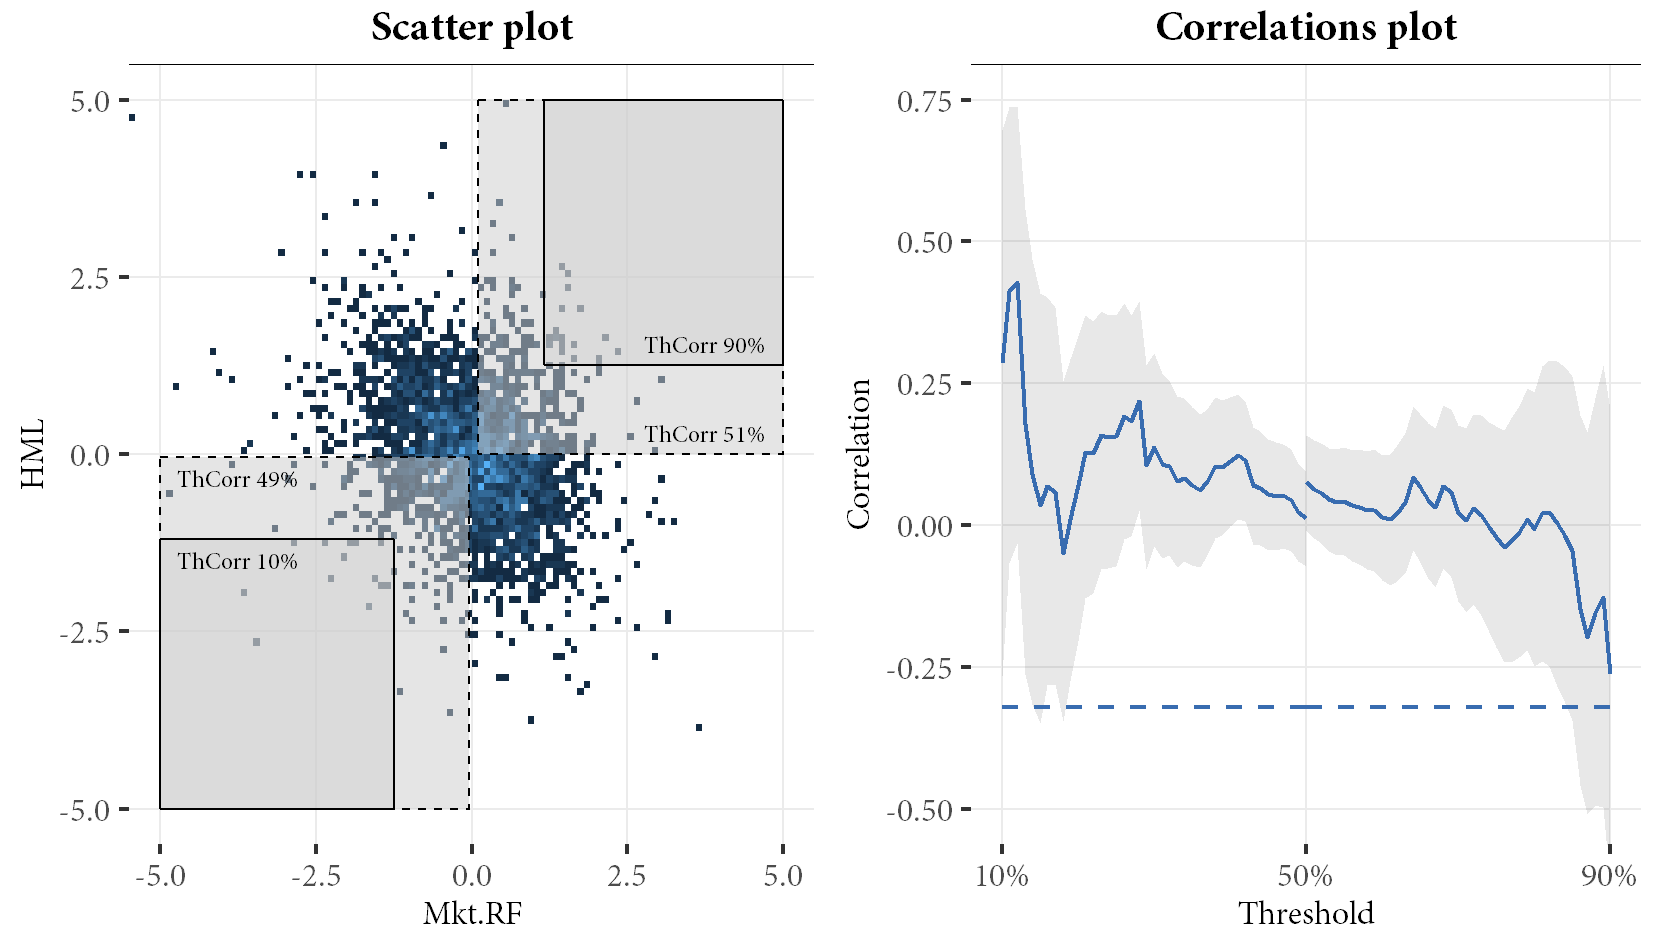
\includegraphics[scale=1]{graphics/threshold_explain_res.png}
  \footnotesize
  \caption{Illustration of threshold correlations}
  \begin{longcaption}
    ARMA-GARCH residuals from the Mkt.RF--HML asset pair. 95\% shaded confidence bounds. The unconditional correlation is given by the dashed line. Based on weekly data 1963--2016.
  \end{longcaption}
  \label{fig:illustrate_threshold}
\end{figure}

We now plot threshold correlations without the adjacent scatter graph. \autoref{fig:threshold1} displays threshold correlations for HML, CMA and RMW against each other as well as against the the other factors Mkt.RF, SMB and Mom. We note that for most asset pairs, the threshold correlation is significantly different from the unconditional correlation coefficient given by the dashed line.

We also note that there is asymmetry around the median for some factor pairs, including the Mom--CMA, RMW--HML, RMW--CMA, and to a lesser extent Mkt.RF--RMW, asset pairs. For example, in the Mom-CMA asset pair, the threshold correlation jumps up for the first percentile below the median, indicating that the correlation is higher when both realize below the median than when both realize above the median. This type of asymmetric property, where downside (below the median) correlation is higher than upside correlation is unwanted, as it reflects a poorer diversification in bad times. The opposite type of asymmetry can be seen for the HML--RMW and CMA--RMW asset pairs; When these factors simultaneously realize above the median, they are significantly more correlated. This pattern presents no diversification problem.

Although estimated with substantial uncertainty, the threshold correlations do not seem to be constant as the threshold $p$ approaches either zero or one. For example, the Mkt.RF--HML asset pair seems to have a downward pattern, where correlations are the most positive in the lowest percentiles of residuals and the most negative in the highest percentiles of residuals. In fact, this pattern is unwanted from a diversification perspective, as series tend to coincide more in extreme negative events. 

The CMA--HML pair stands out from the other factors. The pair exhibits an unusually high correlation in excess of $0.60$ with a virtually flat threshold pattern. HML and CMA are also generally similar to each other in their respective threshold patterns to other factors -- most notably in the HML/CMA--RMW pairs. They differ in the presence of a break around the median in Mom--CMA not present in Mom--HML.

RMW is the only factor to be virtually uncorrelated with Mkt.RF in the lower tails, suggesting that it is a good diversifier in market downturns. This is very different from the pattern of higher threshold correlations as $p$ approaches zero for e.g. Mkt.RF--HML. For Mkt.RF--HML, the higher lower tail correlation could be related to the industry over-capacity hypothesis discussed in~\autoref{sec:literature}, i.e. that value firms are particularly sensitive to market downturns due to unproductive capital.

While the patterns in threshold correlations are interesting, we are careful not to draw conclusions regarding diversification benefit based on solitary threshold correlation graphs -- what is interesting is the total pattern, and our key point is that there seems to be tail dependence that should not be ignored in the copula specification.

\begin{figure}[p]
  \centering
  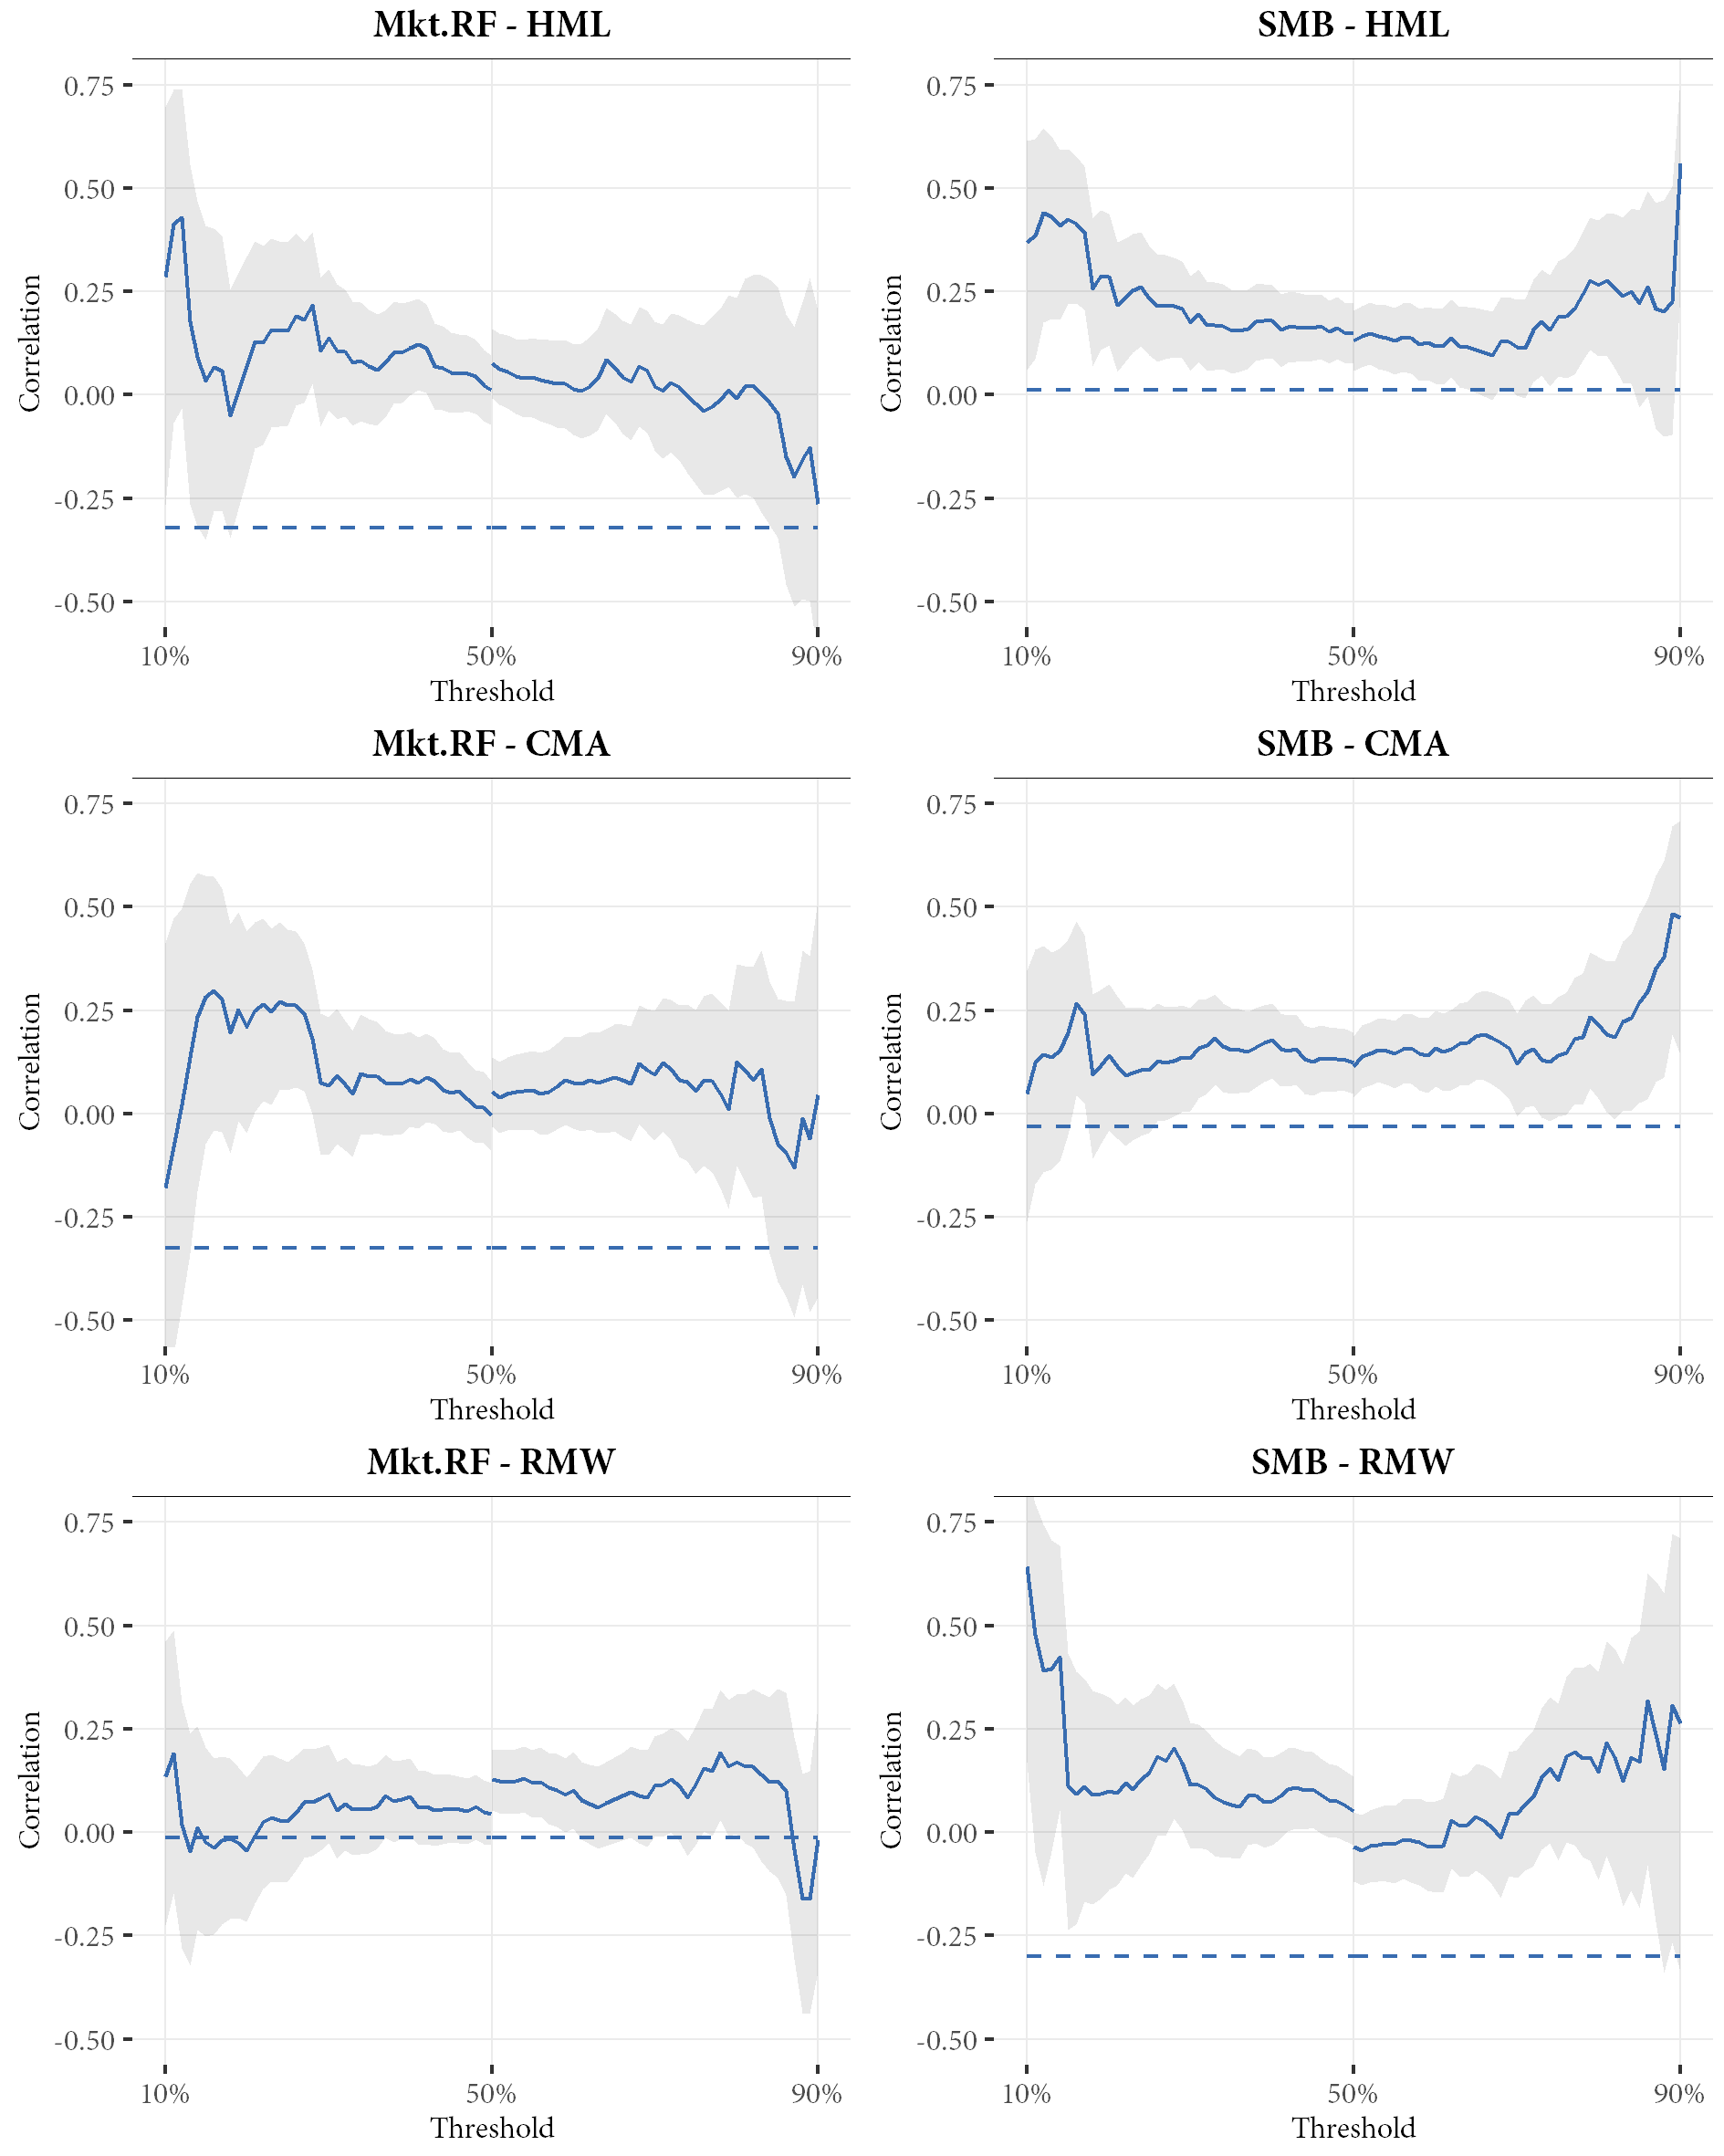
\includegraphics[scale=1]{graphics/threshold1.png}
  \footnotesize
  \caption{Threshold correlations of ARMA-GARCH standardized residuals}

  \begin{longcaption}
    The formula for threshold correlations for a threshold $p$ is given in~\autoref{eq:th_corr}. 95\% shaded confidence bounds, taking the model as given. The unconditional correlation is given by the dashed line. Based on weekly data 1963--2016.
  \end{longcaption}
  \label{fig:threshold1}
\end{figure}
\begin{figure}[p]
  \ContinuedFloat
  \centering
  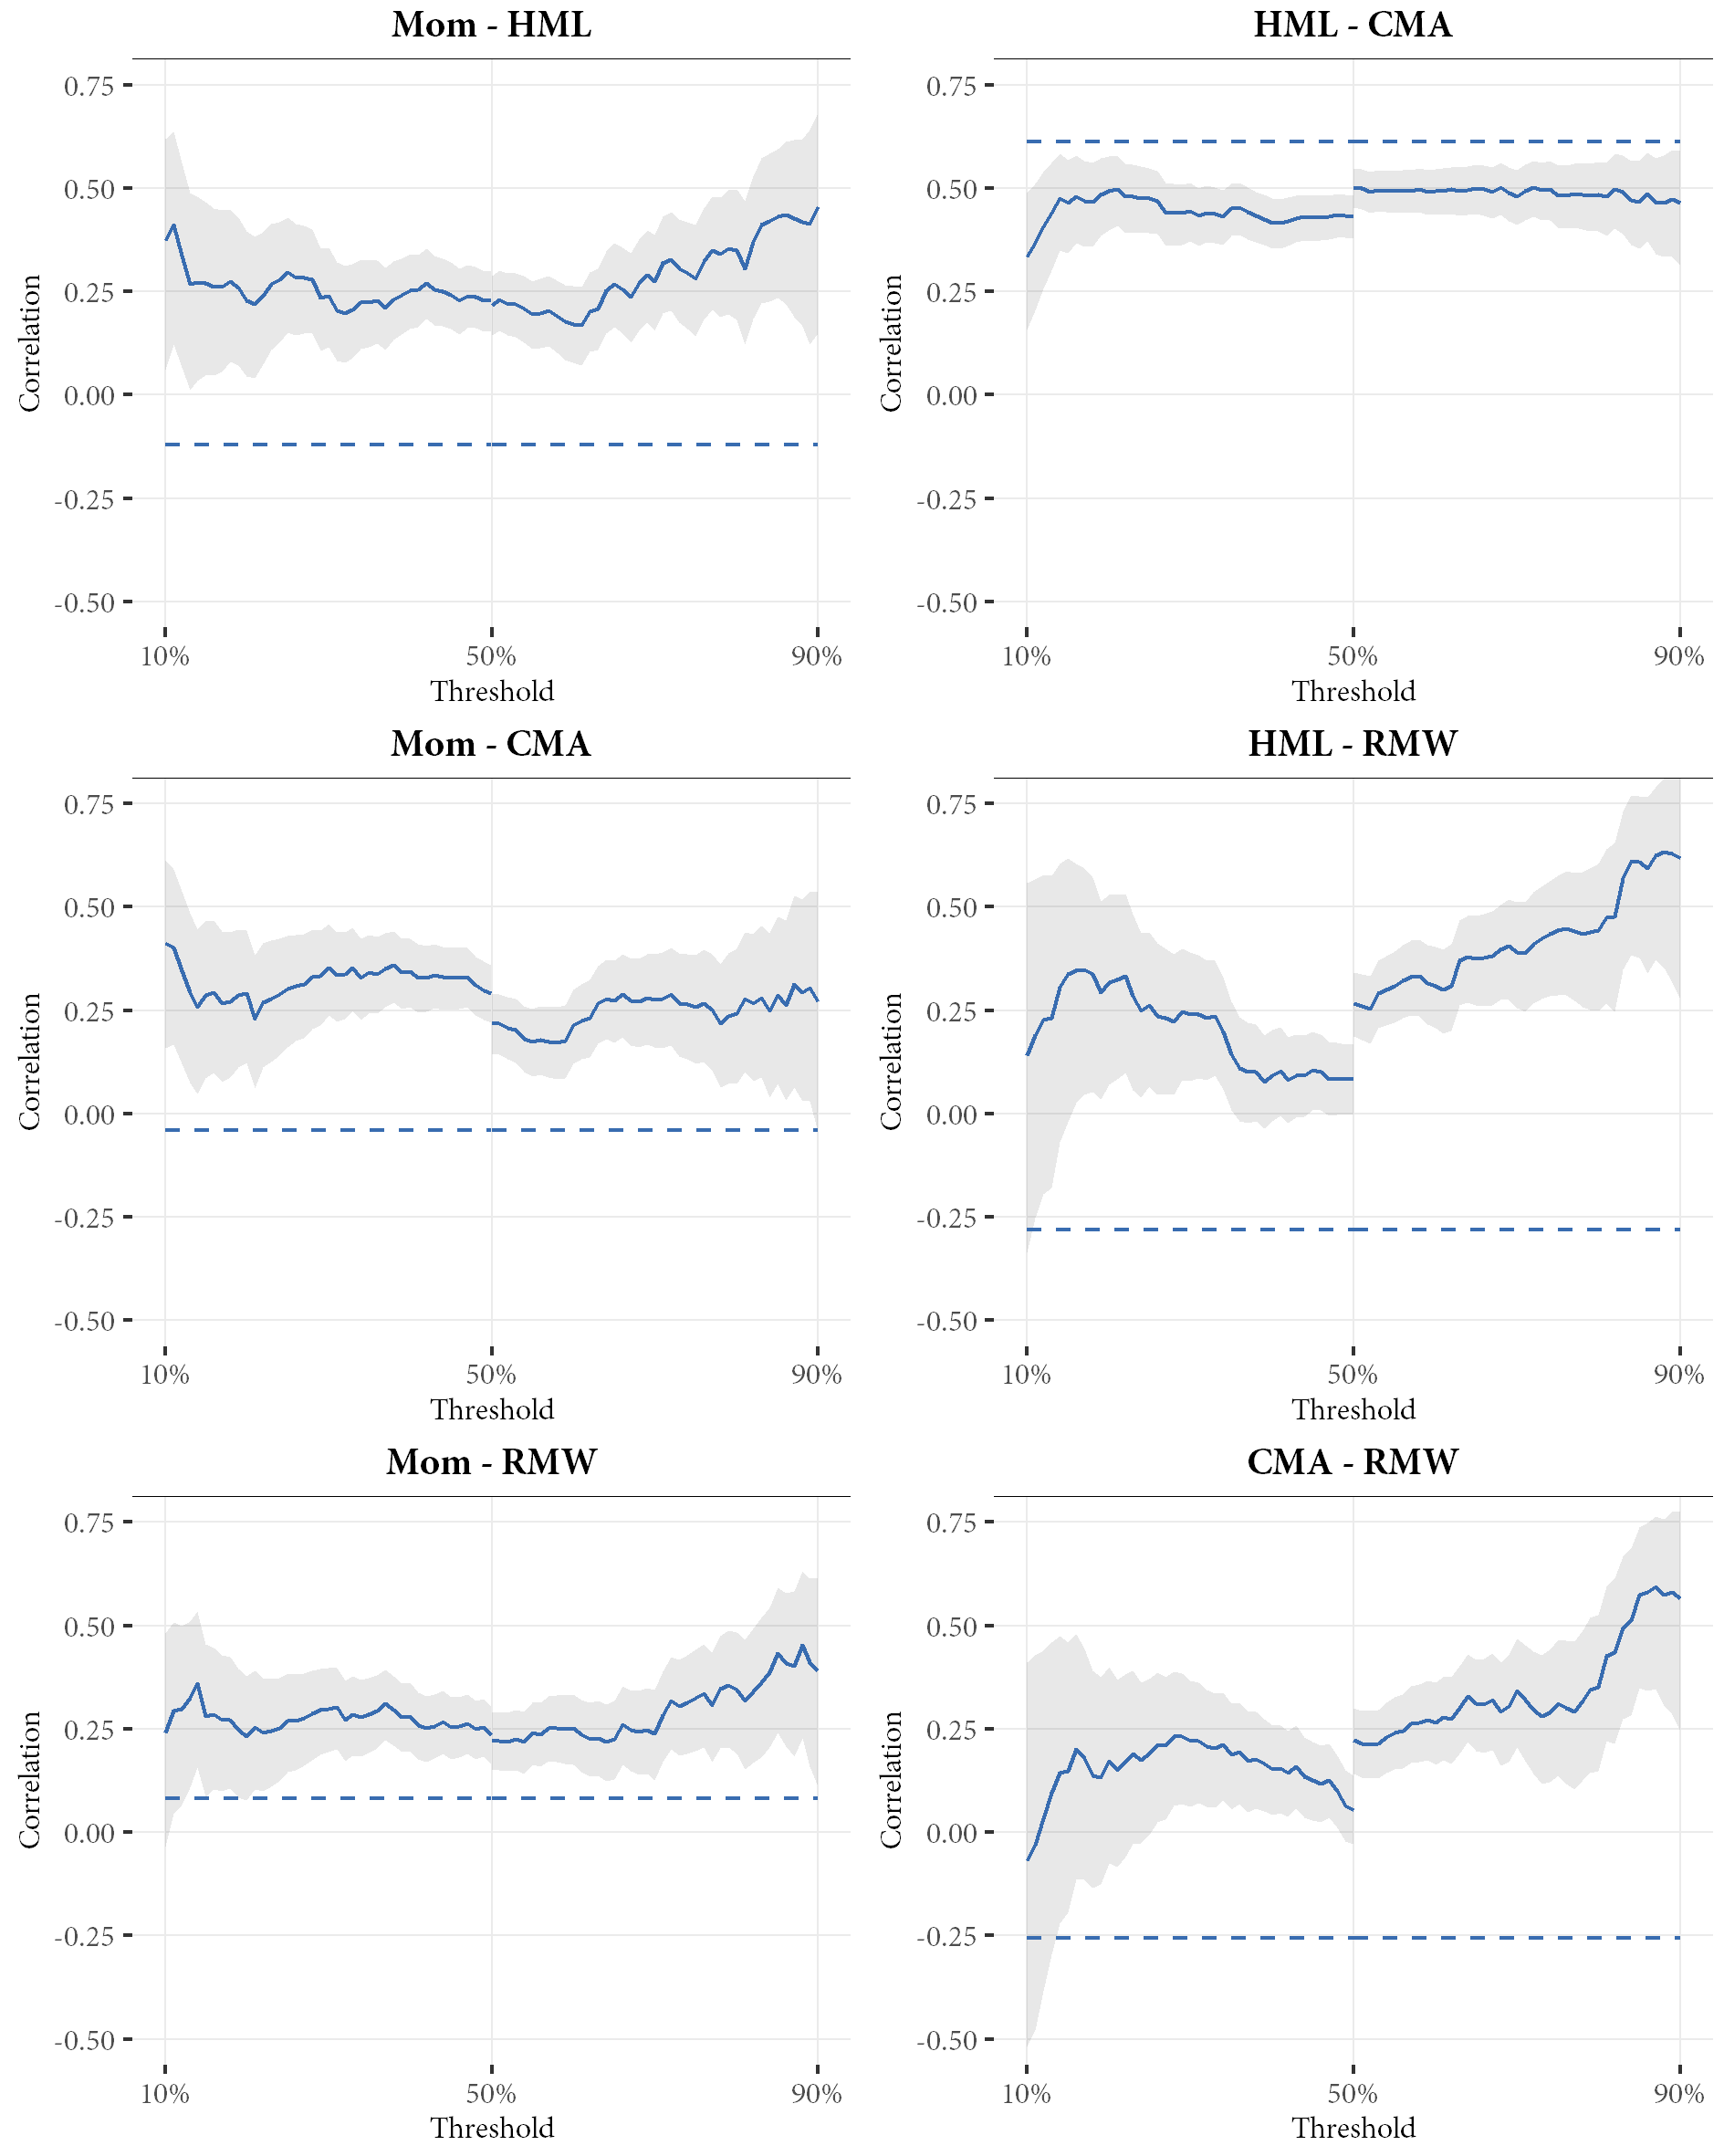
\includegraphics[scale=1]{graphics/threshold2.png}
  \footnotesize
  \caption{Threshold correlations of ARMA-GARCH standardized residuals (cont.)}
\end{figure}

\subsubsection{Rolling correlations}

We compute rolling 52-week correlations between the factors on standardized residuals of our ARMA-GARCH models, according to the formula: 
\begin{align}
    RCorr(r_{i, t}, r_{j, t})_t^{52} = \frac{\sum^{t}_{t-51}(r_{i, t} - \bar{r}_i)(r_{j,t} - \bar{r}_j)}{\sqrt{\sum^{t}_{t-51} (r_{i,t} - \bar{r}_i)^2} \sqrt{\sum^{t}_{t-51} (r_{j,t} - \bar{r}_j)^2}}
\end{align}
where $r_i$, $r_j$ are the different pairs of the factor strategies' ARMA-GARCH residuals.\footnote{Rolling correlations for the returns themselves are available in the \autoref{app:supplementary}.} Results are presented in ~\autoref{fig:rolling1}.
% plots
\begin{figure}[!p]
  \centering
  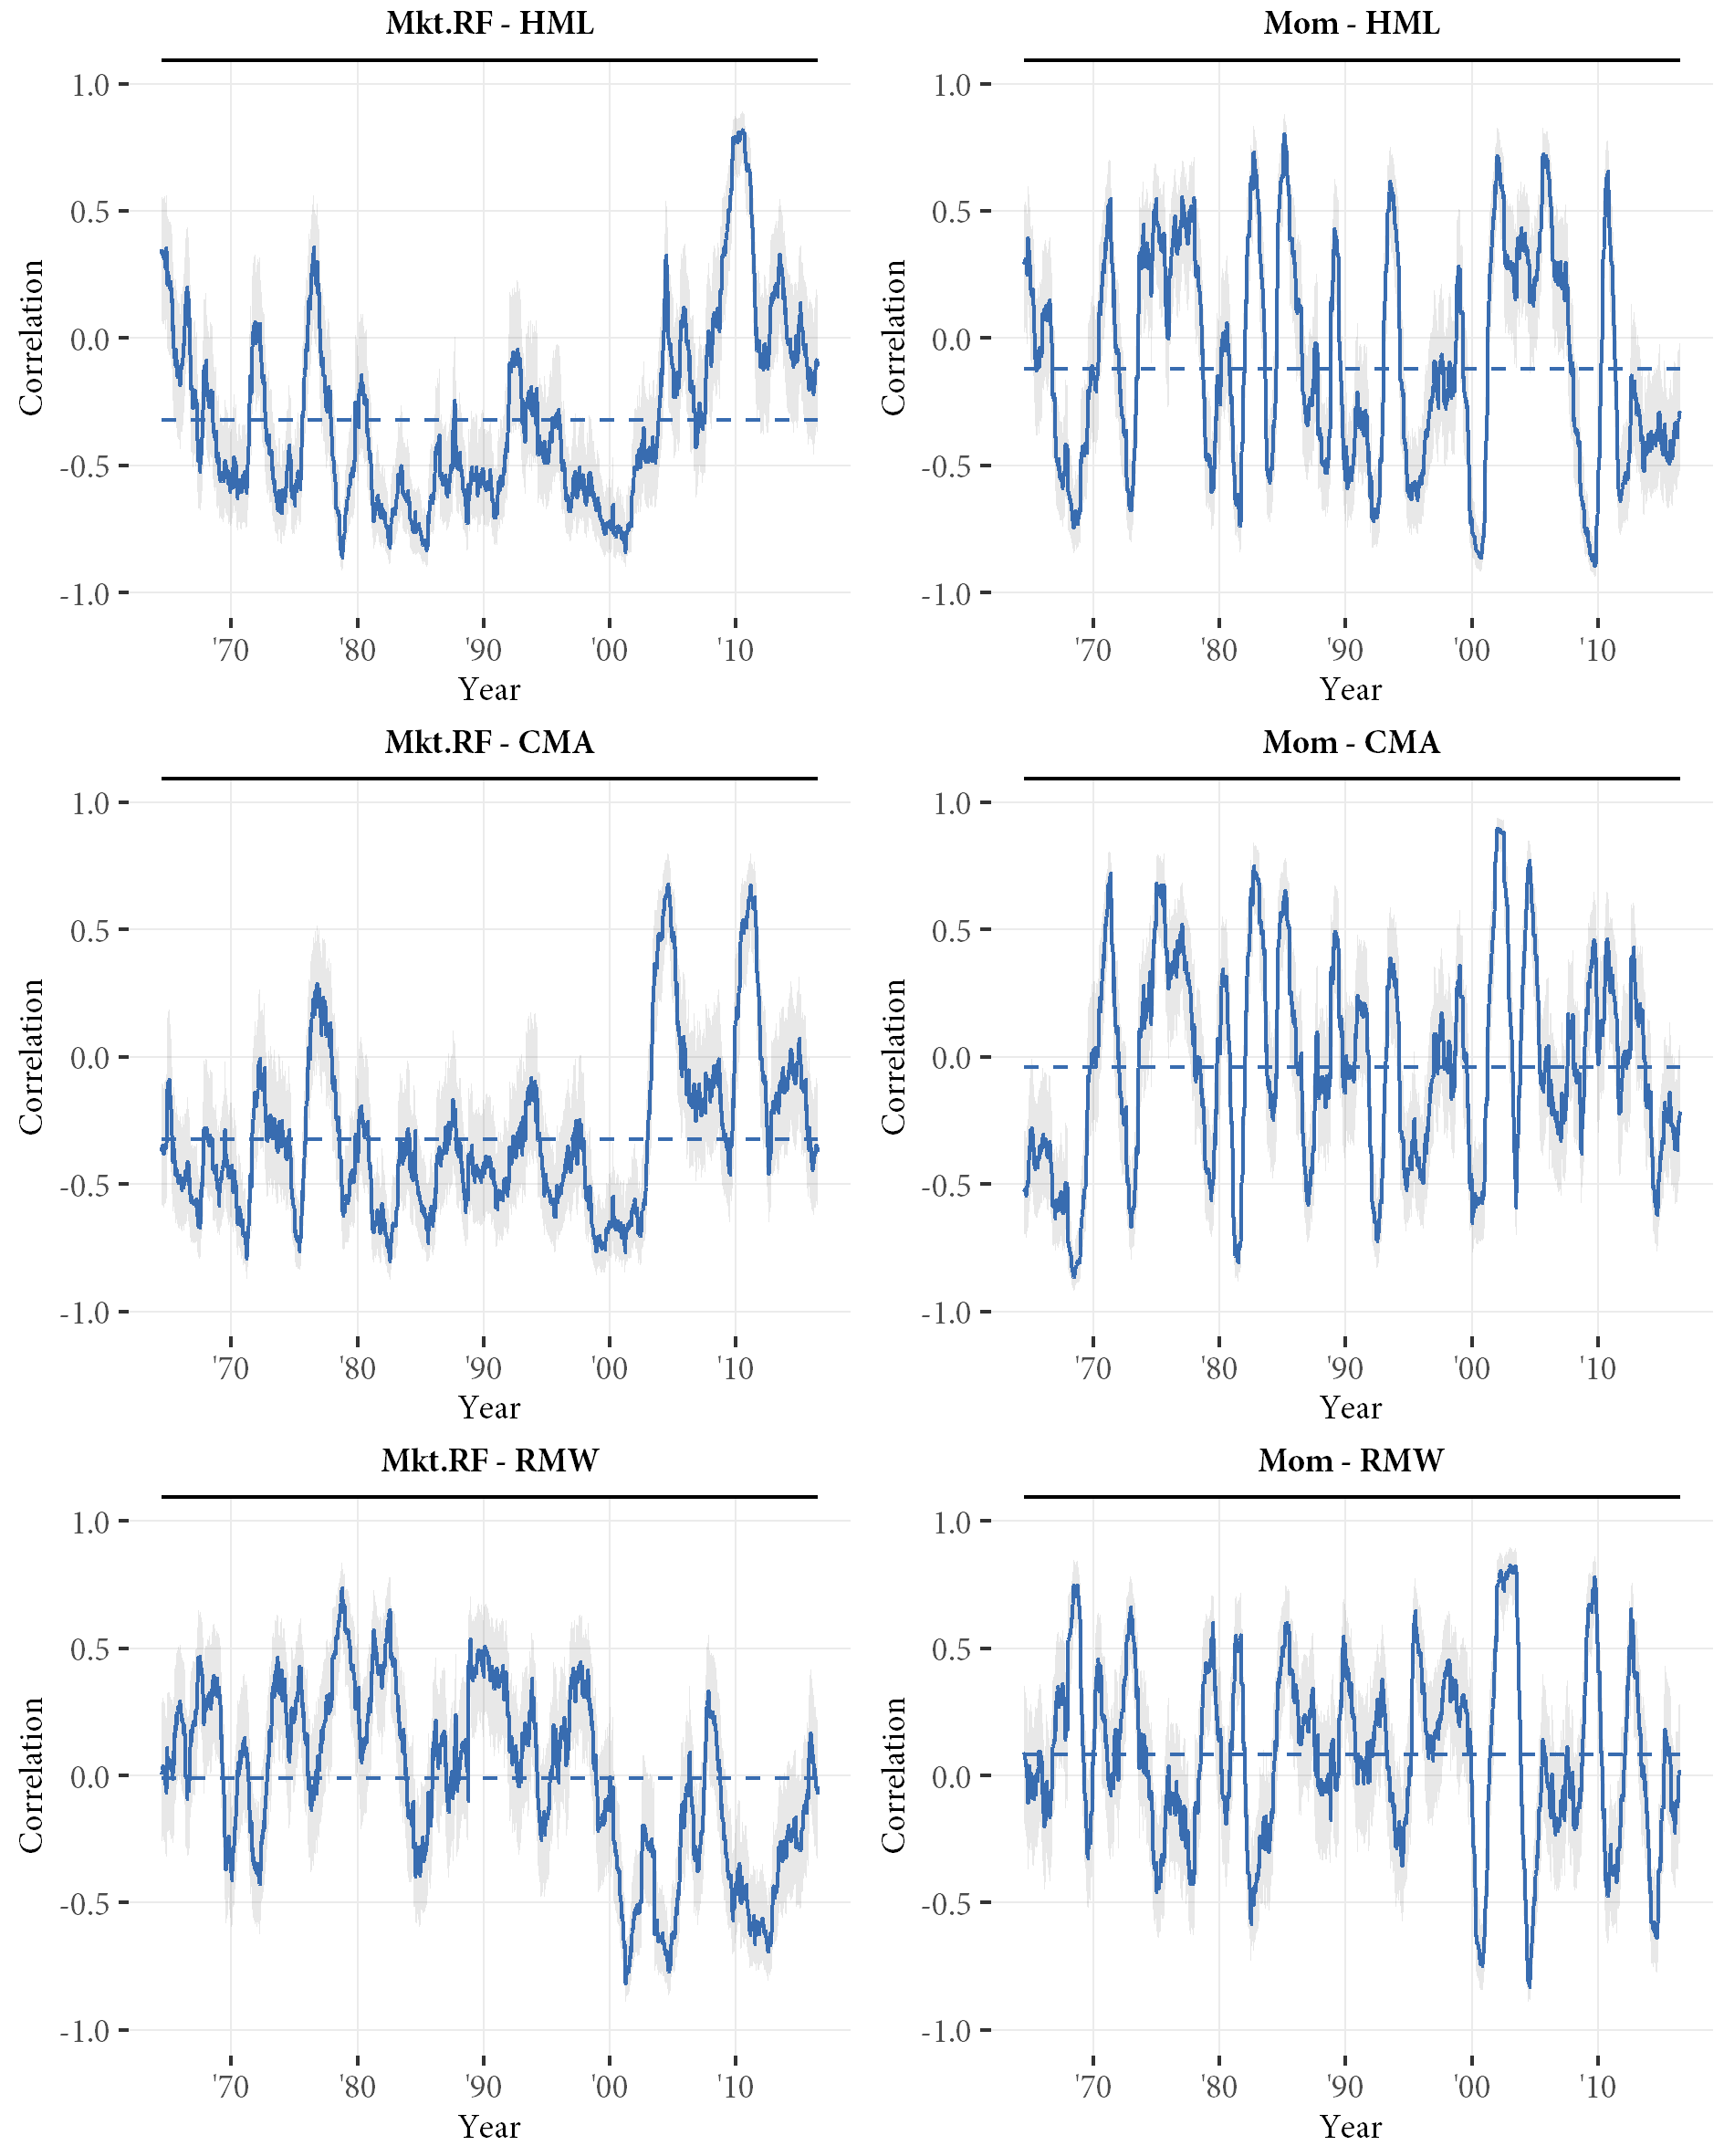
\includegraphics[scale=1]{graphics/rolling1.png}
  \footnotesize
  \caption{Rolling correlations of ARMA-GARCH standardized residuals}
  \begin{longcaption}
    95\% shaded confidence bounds, taking the model as given. The unconditional correlation is given by the dashed line. Based on weekly data 1963--2016.
  \end{longcaption}
  \label{fig:rolling1}
\end{figure}
\begin{figure}[!p]
  \ContinuedFloat
  \centering
  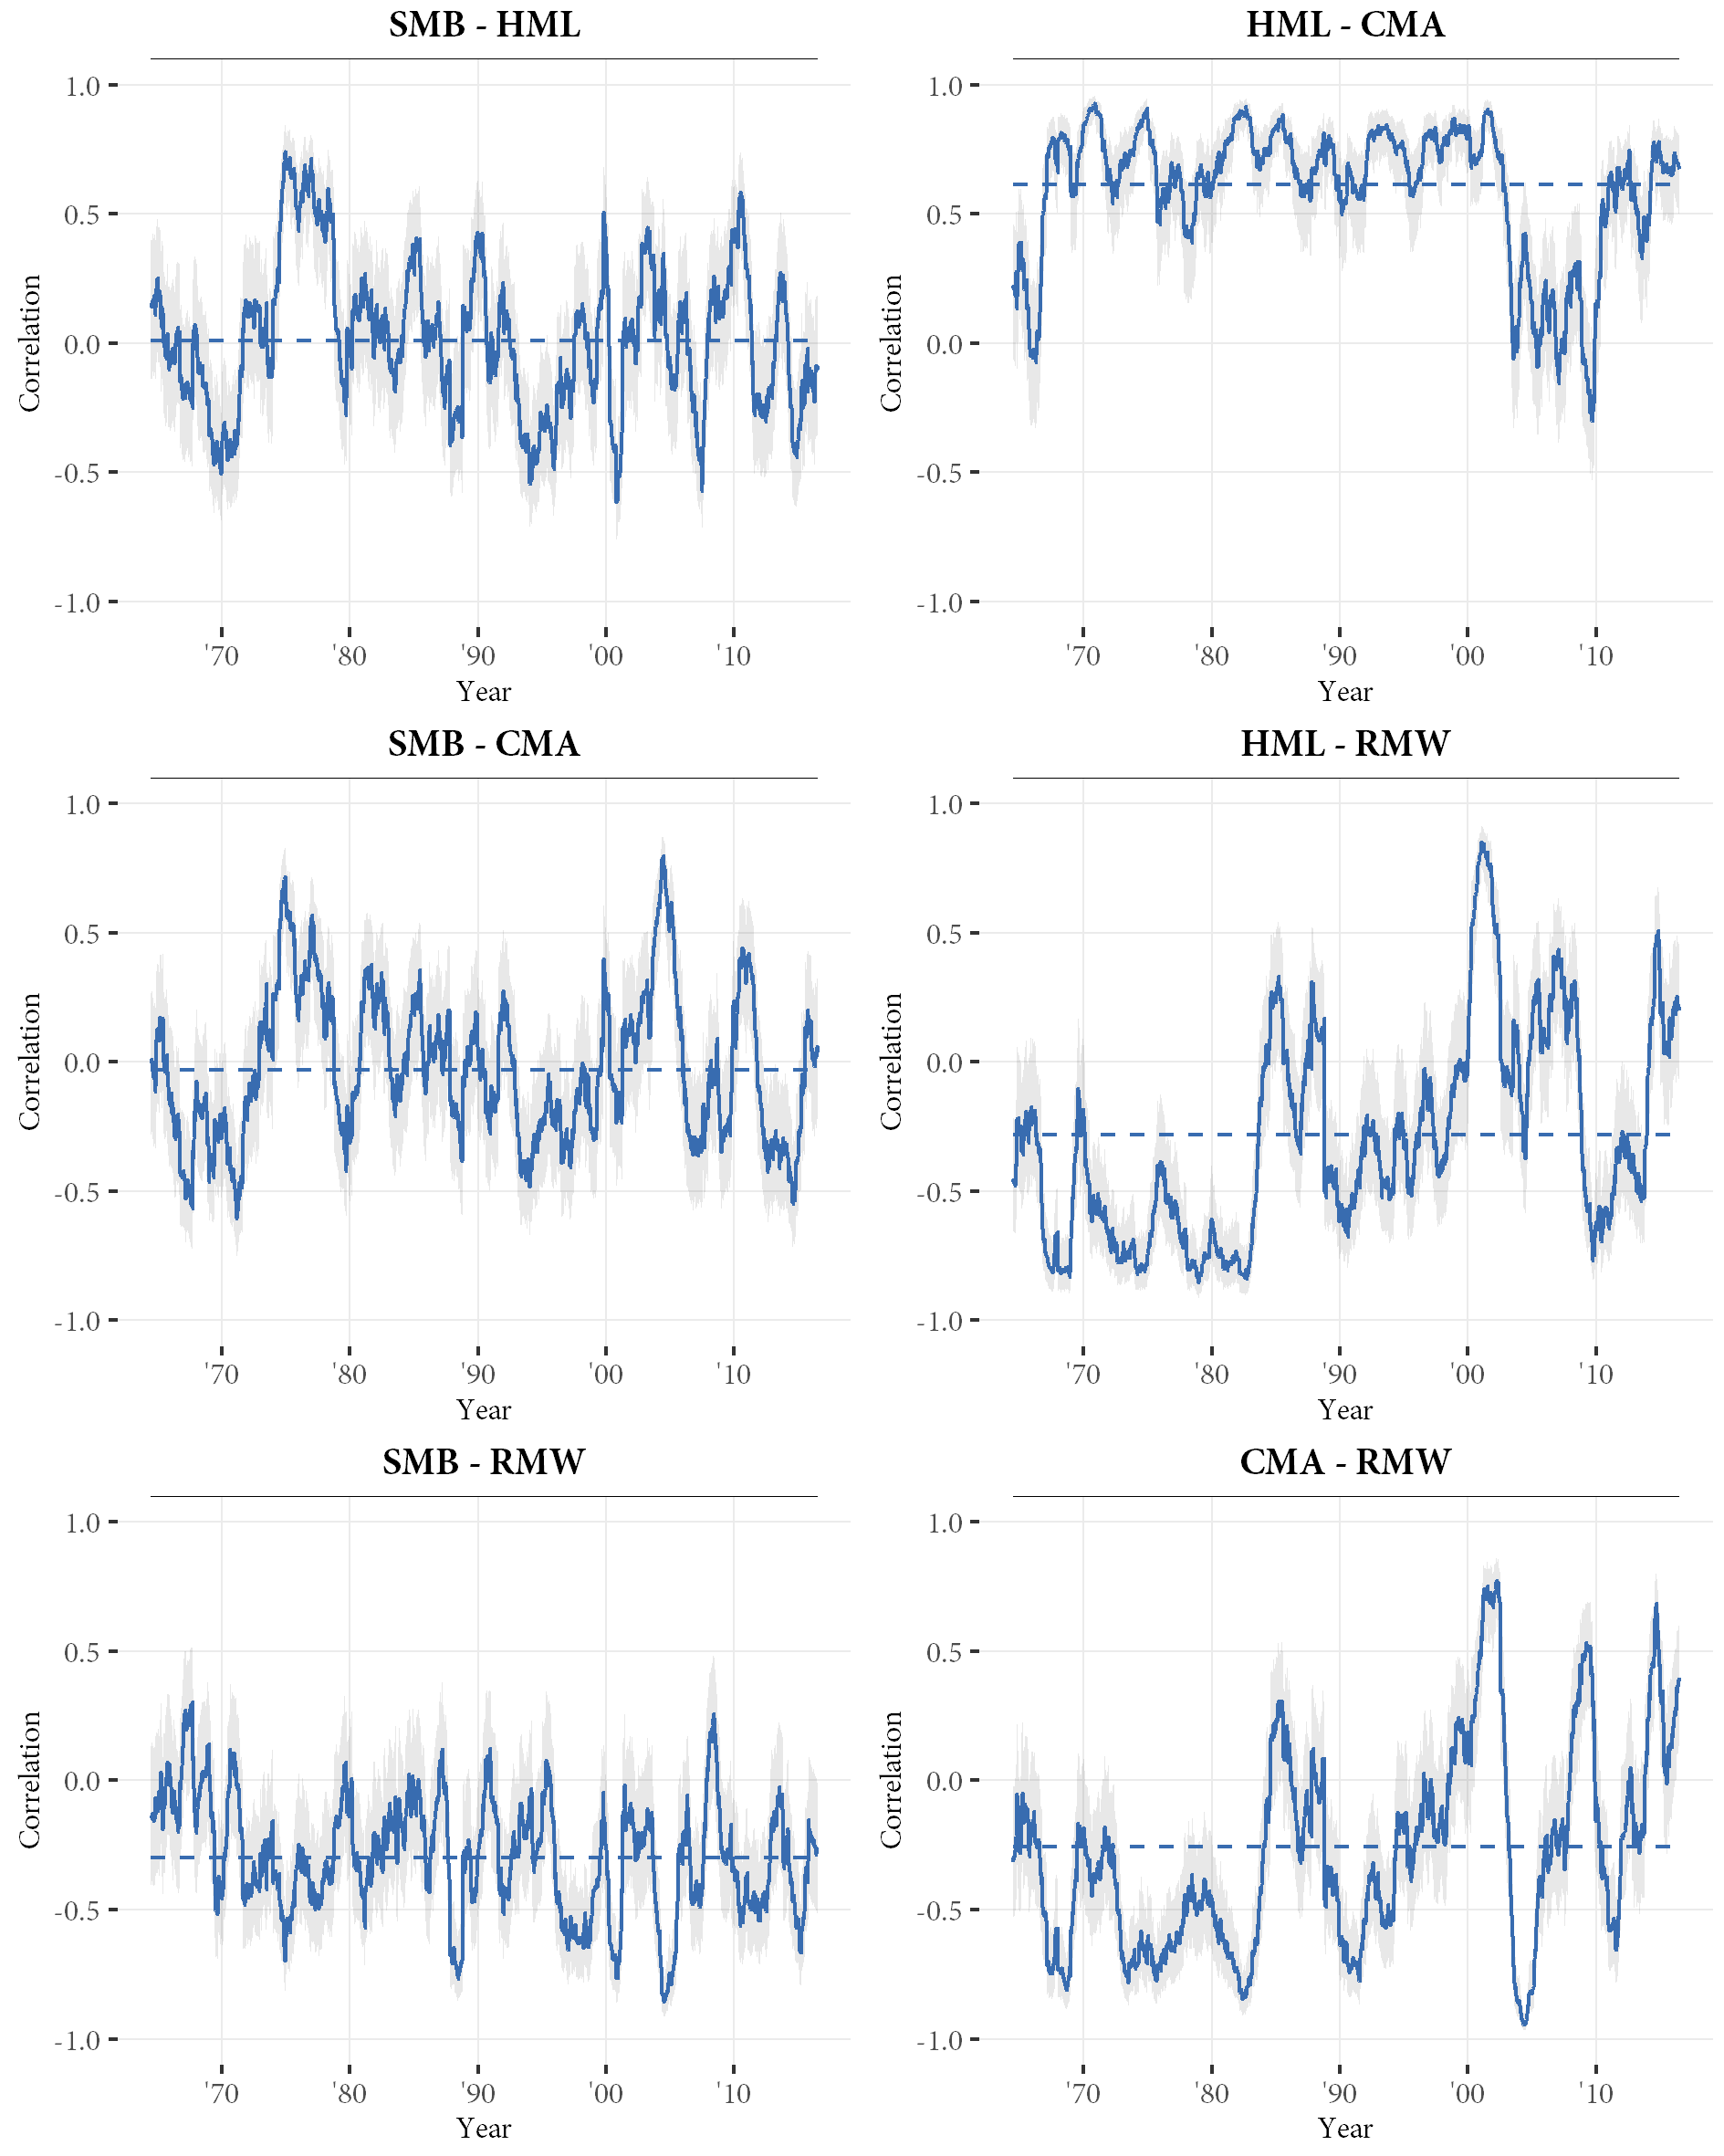
\includegraphics[scale=1]{graphics/rolling2.png}  
  \footnotesize
  \caption{Rolling correlations of ARMA-GARCH standardized residuals (cont.)}
\end{figure}
% talk
First, we note that for most factor pairs, the rolling 52-week correlations are time-varying, and indeed appear to swing wildly. The unconditional correlation of Mkt--HML is negative in the studied time period, but rolling correlations range between -0.75 and 0.75. Also of note is the momentum factor's rapid shifts between positive and negative correlations to the other factors. 

% Value and profitability in crisis times?
Second, by visual inspection, we see no obvious trend in the correlations between factor pairs. There are, however, notable patterns around the 2000--2001 bubble period -- here, the correlations of HML--RMW, CMA--RMW and Mkt--CMA appear to jump sharply. This is an indication that diversification benefits may be time-varying. Another interesting pattern is that the correlations of Mkt--RMW went down sharply around this period -- in line with the idea that profitable firms are stronger and better at weathering crises than the average firm~\autocite{NovyMarx2013}. The 2000--2001 period may represent a structural break in the dependency patterns between factors, with the appearance of persistent differences before and after -- however, there is not enough post-2000 data to support such a conclusion, yet.

Third, the HML--CMA factor pair again stands out as different from other factor pairs. The unconditional correlation is much closer to the rolling estimates than for other factor pairs, with a dip in the 2000--2010 period that appears to have gone away. Clearly, the HML--CMA pair is the most strongly correlated factor pair, even when considering subperiods of the data.

Our key takeaway from the rolling correlations is that there seems to be persistency in the time-variation in correlations. This could be incorporated in the copula specification, which then needs to have a time-varying correlation matrix, $\Psi_t$.

% \subsubsection{Takeaways from Analysis of Multivariate Dependence}

% Univariate residuals appear to be white noise series with no remaining autocorrelation or volatility clustering. However, there is important dependence between residuals of different strategies. First, threshold correlations show that there is tail dependence -- in times when factor pairs simultaneously realize in their best and worst percentiles, correlations are significantly different from the unconditional correlations. In fact, threshold correlations are substantially higher than the unconditional correlations, which indicates that diversification benefits are smaller than expected when factors simultaneously experience bad (or good) times. Second, rolling correlations show that correlations between series are highly time-varying and seem to exhibit persistence. A copula model that incorporates both tail dependence and time-varying dependence is likely to improve on the description of joint returns.

% Both analyses also show that the HML-CMA asset pair is quite different from the other pairs, exhibiting a much higher and more stable dependence. Differently put, they look quite similar as opposed to any other factor pair, and the merit of including both in factor portfolios seems more unclear.

\label{sub:threshold_and_rolling_correlations_of_residuals}

% subsection threshold_and_rolling_correlations_of_residuals (end)
 % threshold and rolling

%!TEX root = ../main.tex
\subsection{Copula specification and estimation results}
Given the results of the dependence structure of residuals, we now discuss the best choice of copula model and present estimation results of the six competing copula specifications.

We have estimated constant and dynamic normal, symmetric \emph{t} and skewed \emph{t} copula models on the full dataset of uniform GARCH residuals. Results are presented in~\autoref{tab:copula_estimation}. 

First, we examine the choice between a normal, symmetric \emph{t} or skewed \emph{t} copula. We note that $\nu_c$ is clearly significant and suggests one of the Student's \emph{t} models with tail dependence over the normal model. Second, we examine the asymmetric specification and find that few of the $\gamma_c$ estimates appear significant. This indicates that the asymmetry is hard to capture, or that it is not well represented by this type of model. This is supported by the relatively small improvement in log-likelihood in going from a symmetric \emph{t} to skewed \emph{t} copula, and also by the fact that the BIC criterion prefers the symmetric \emph{t} model in the dynamic case. 

Second, we examine the choice between a constant and dynamic copula correlation matrix. There is a significant improvement in log-likelihood and BIC when moving from a constant to a dynamic copula, which suggests that time-varying dependence shown by rolling correlation is captured and improves the model's fit. We also find a high persistence of the correlation process, as $\alpha + \beta$, is close to a unit root.

In summary, we find that the dynamic symmetric \emph{t} copula is the best specification, as it has the lowest BIC, well defined parameters, and is strongly supported by the dependence pattern showcased by threshold and rolling correlation analyses. While the skewed \emph{t} copula is an interesting model, we believe that the asymmetry patterns in data are too irregular to be well captured by a copula model with only one asymmetry parameter for each series (this is further discussed in the subsequent robustness discussion, see \autoref{sub:05_robust}).

%!TEX root = ../../main.tex

\begin{table}[!ht]
  \centering
  \scriptsize
  \renewcommand{\arraystretch}{1.2}

  \caption{Parameter estimates for copula models based on uniform residuals from ARMA-GJR-GARCH models.\\ \quad \\
  Stationary bootstrap standard errors in parentheses, following Politis and Romano (1994). Copula parameters: $\nu_c$ is the degree of freedom, $\gamma_c$ is the vector of skewness parameters, $\alpha$, $\beta$ are the shock loading and autoregressive loading of the cDCC process. The significance test of $\nu_c$ is based on $1/\nu_c$, as this ratio goes to zero when $\nu_c$ goes to infinity (normality). Sample: 1963-07-05--2016-07-01.}
  \begin{tabularx}{\textwidth}{@{}l ddd X ddd @{}}
    \toprule
    &
      \multicolumn{3}{c}{Constant Copula} &&
      \multicolumn{3}{c}{Dymamic Copula} \\
    \cmidrule{2-4} \cmidrule{6-8}
    &
      \multicolumn{1}{c}{Normal} & \multicolumn{1}{c}{Symmetric \emph{t}} & \multicolumn{1}{c}{Skewed \emph{t}} & &
      \multicolumn{1}{c}{Normal} & \multicolumn{1}{c}{Symmetric \emph{t}} & \multicolumn{1}{c}{Skewed \emph{t}} \\
    \midrule
    $\nu_c$ & & 6.625^{**} & 6.671^{**} && & 11.936^{**} & 11.881^{**} \\
    & & (0.636) & (0.264) && & (0.770) & (0.641) \\
    \\
    $\gamma_\text{Mkt}$ & & & -0.057 && & & -0.078 \\
    & & & (0.047) && & & (0.062) \\
    \\
    $\gamma_\text{HML}$ & & & 0.103 && & & 0.083 \\
    & & & (0.036) && & & (0.071) \\
    \\
    $\gamma_\text{SMB}$ & & & -0.103 && & & -0.175 \\
    & & & (0.055) && & & (0.098) \\
    \\
    $\gamma_\text{Mom}$ & & & -0.202^{**} && & & -0.145 \\
    & & & (0.032) && & & (0.073) \\
    \\
    $\gamma_\text{RMW}$ & & & 0.021 && & & 0.095 \\
    & & & (0.035) && & & (0.058) \\
    \\
    $\gamma_\text{CMA}$ & & & 0.076 && & & 0.001 \\
    & & & (0.038) && & & (0.050) \\
    \\
    $\alpha$ & & & && 0.065 & 0.068^{**} & 0.068^{**} \\
    & & & && (0.006) & (0.006) & (0.006) \\
    \\
    $\beta$ & & & && 0.915 & 0.913^{**} & 0.913^{**} \\
    & & & && (0.008) & (0.007) & (0.007) \\
    \midrule
    Log-likelihood & 1169.194 & 1555.683 & 1572.672 && 2790.618 & 2977.648 & 2989.273 \\
    No. of Parameters & 15 & 16 & 22 && 17 & 18 & 24 \\
    % BIC & -348.32 & -122.21 & -316.432 && -243.221 & -342.342 & -396.324 \\
    Persistence & & & && 0.981 & 0.981 & 0.981 \\
    \bottomrule
  \end{tabularx}

  \label{tab:copula_estimation}
\end{table}
 % estimation results and explaining parameterization choice

%!TEX root = ../main.tex
\subsection{Copula robustness check}
\label{sub:05_robust}

This subsection provides an in-sample robustness check of how well the copula models can reproduce the threshold correlations and rolling correlations found in the dependence analysis of ARMA-GARCH residuals. By comparing simulated data from the copulas to ARMA-GARCH residual data, we find that the main features are captured. However, we highlight that tail dependence is only reproduced to a certain extent.

\subsubsection{Threshold correlations in constant copulas}
By simulating 250,000 weeks of shocks in the copula, and then transforming these shocks into standardized residuals for each of the factors, we can test the constant \textit{t} copulas' abilities to generate the threshold correlations in the ARMA-GARCH residuals.\footnote{This robustness check is inspired by \textcite{ChristoffersenLanglois2013}.} If a Student's \textit{t} copula specification reasonably well captures tail dependence, the threshold correlations from the empirical and the copula specification should align. The results are presented in~\autoref{fig:threshold_simulated1}.

\begin{figure}[!ht]
  \centering
  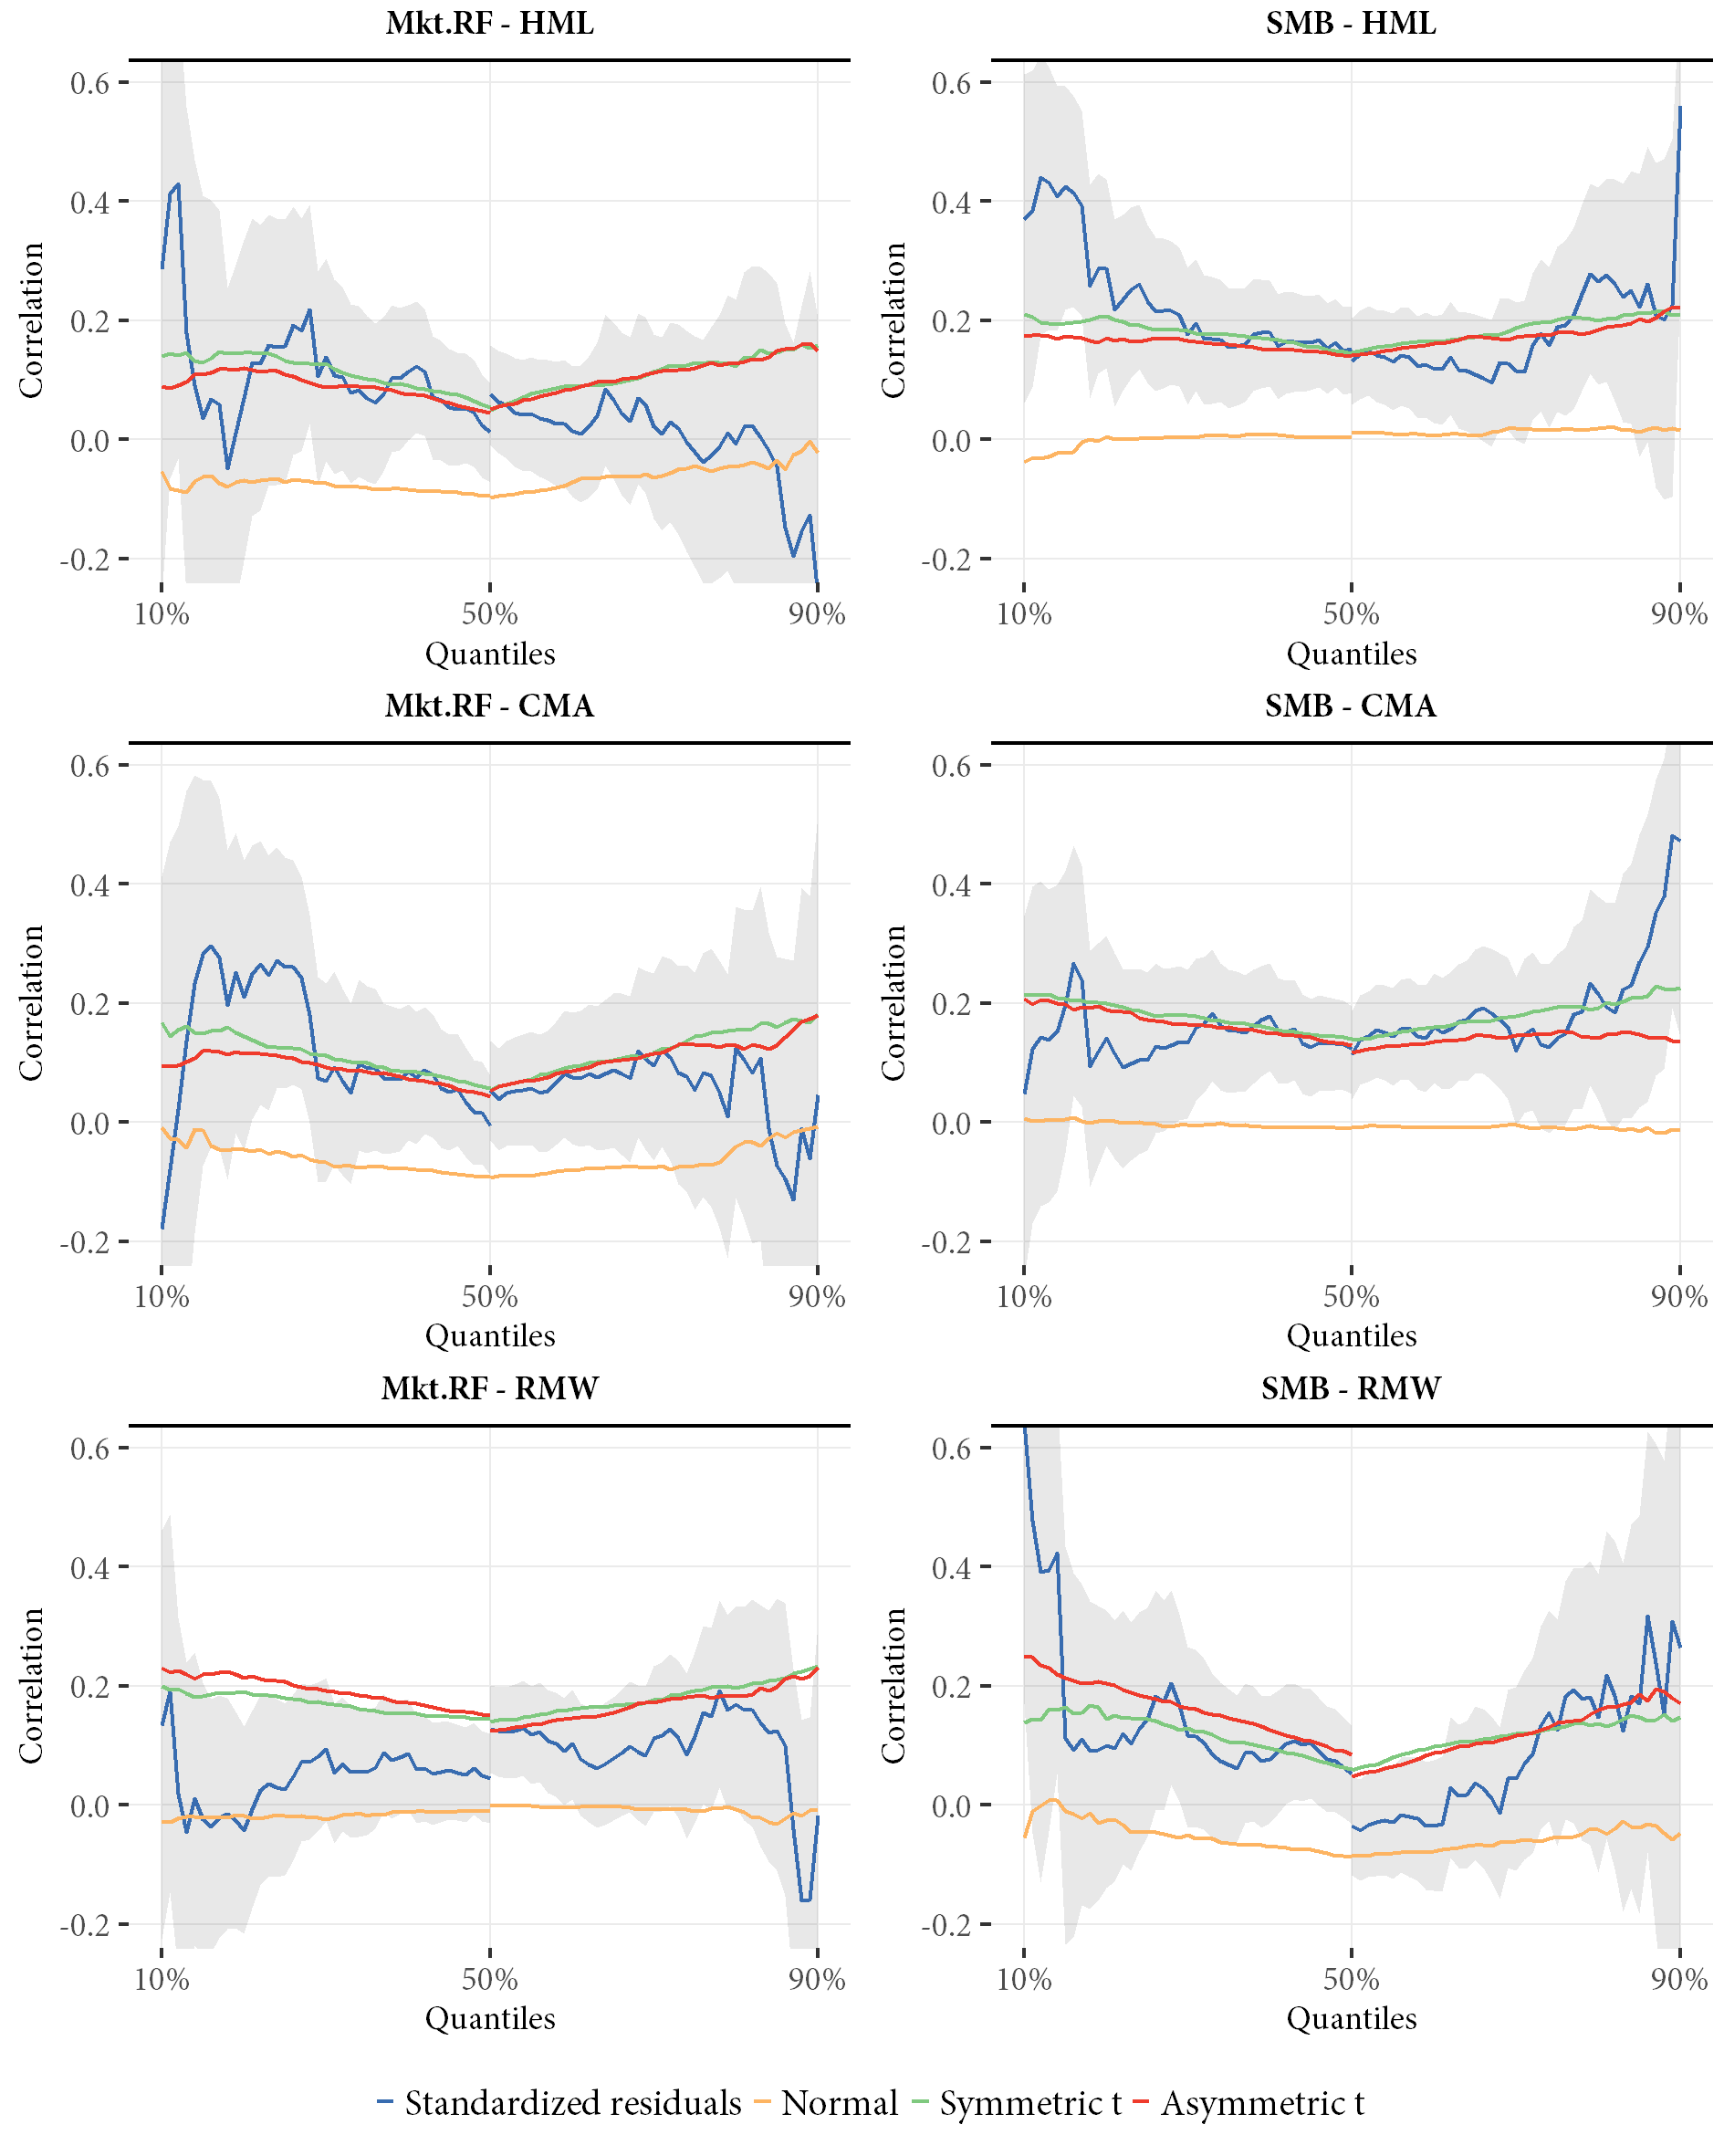
\includegraphics[scale=1]{graphics/threshold_simulated_1.png}  
  \footnotesize
  \caption{Threshold correlations of standardized residuals from the constant copulas}

  \begin{longcaption}
    Threshold correlations of simulated constant copulas, compared to ARMA-GARCH standardized residuals (95\% confidence bounds taking the ARMA-GARCH models as given). The simulated threshold correlations are based on 250,000 simulated returns each. ARMA-GARCH models based on empirical weekly data 1963--2016.
  \end{longcaption}
  \label{fig:threshold_simulated1}
\end{figure}
\pagebreak
\begin{figure}[!ht]
  \ContinuedFloat
  \centering
  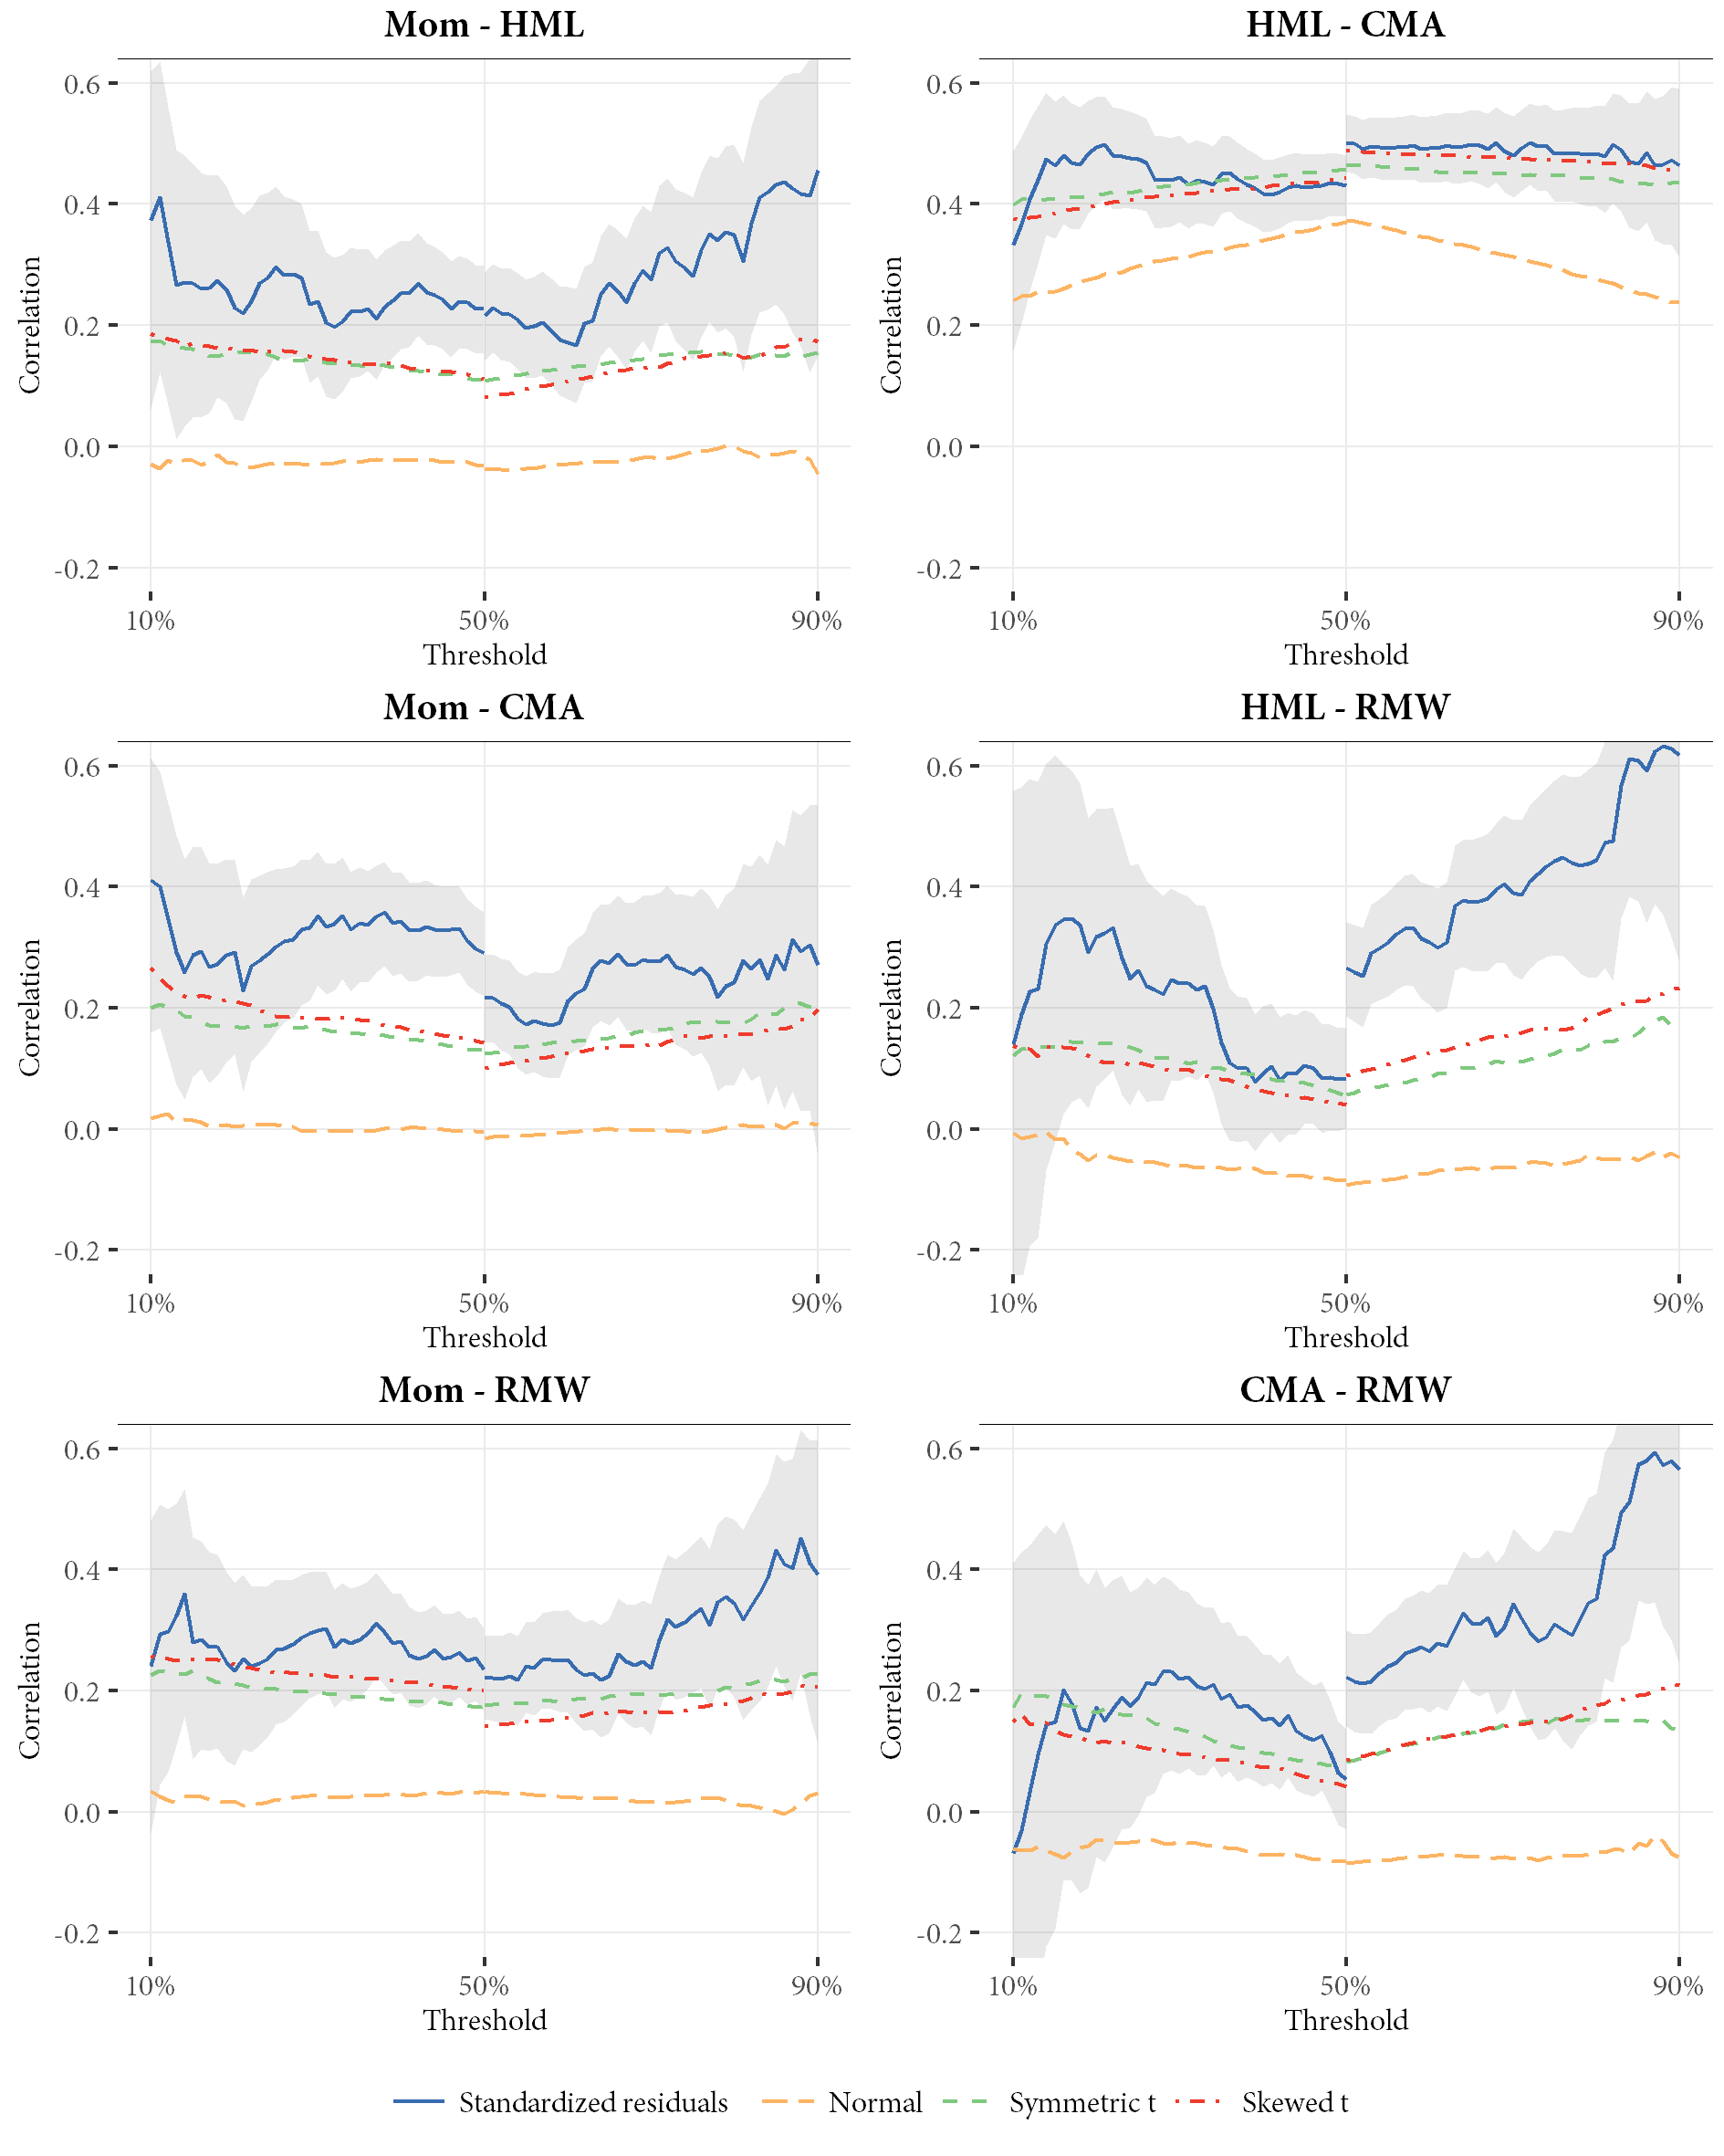
\includegraphics[scale=1]{graphics/threshold_simulated_2.png}  
  \footnotesize
  \caption{Threshold correlations of standardized residuals from the constant copulas (cont.)}
\end{figure}
\pagebreak

First, we note that for most factors, the normal copula is the far away from generating threshold correlations that correspond to the empirical distribution around the median. This is highly expected, as the normal copula does not generate tail dependence, and hence the need for the Student's \textit{t} based copula models. The symmetric \textit{t} and asymmetric \textit{t} copulas better capture the threshold correlations, as the fatter tails of the Student's \textit{t} distribution allows for tail dependence. For example, note how the normal copula generates negative threshold correlations for both the Mom--HML and RMW--HML asset pairs, while the Student's \textit{t} based copulas are much closer to the higher values in the data. On the other hand, the Student's \textit{t} based copulas sometimes seem to overshoot the empirical threshold correlation, as in the Mkt.RF--RMW asset pair.

Second, we find that the skewed Student's \textit{t} generates some asymmetry around the median, which can be seen most clearly for the Mom--RMW and RMW--HML asset pairs. The generated asymmetry does, however, appear to be too small to capture the features of the data.

In conclusion, comparing threshold correlations from empirical data and simulated data shows that the constant copula specifications capture some of the tail dependence.\footnote{Note that, in order to make the threshold correlation comparison valid, we use the constant copula specifications. The dynamic version is still the workhorse for all continued analysis in the mean-variance and diversification benefit sections.} Although the Student's \textit{t} and skewed Student's \textit{t} results do not align perfectly with the data, they constitute clear improvements to the normal copula in modeling tail dependence. We observe that the copula seems to lack flexibility to simultaneously generate all the asymmetries in tail dependence. This is quite expected, as the Student's \textit{t} copula only has one degree of freedom parameter that controls the fatness of tails, and the skewed Student's \textit{t} copula only has one skewness parameter for each series. This imposes limits on how strongly the model can express fat tails or asymmetries between factors A and B and simultaneously express other fat tails or asymmetries (or lack thereof) between factors A and C. For a collection of six factors with heterogenous dependence, this is even harder. This is a clear limitation of our quite parsimonious multivariate distribution copula approach. In this regard, vine copulas that allow for unique bivariate copula specifications, as discussed in \autoref{sub:05_01_choosing}, could be the solution.

Although imperfect, the multivariate copula modeling of tail dependence could constitute a significant improvement to alternatives, especially in the field of risk management, where understanding of tail events is paramount.

\subsubsection{Rolling correlations in the dynamic copula}

In-sample, we simulate 10,000 standardized residuals for each week from the estimated dynamic symmetric Student's \textit{t} copula model, and compute the rolling 52-week correlations. This is done to ascertain ourselves that the chosen copula specification does in fact capture the time-variation in correlations. The comparison is made between standardized residuals from the simulated copula model and standardized residuals from the ARMA-GARCH model of univariate series. If satisfactory, the rolling correlations of the copula model and the ARMA-GARCH univariate models will be roughly the same.

\begin{figure}[!ht]
  \centering
  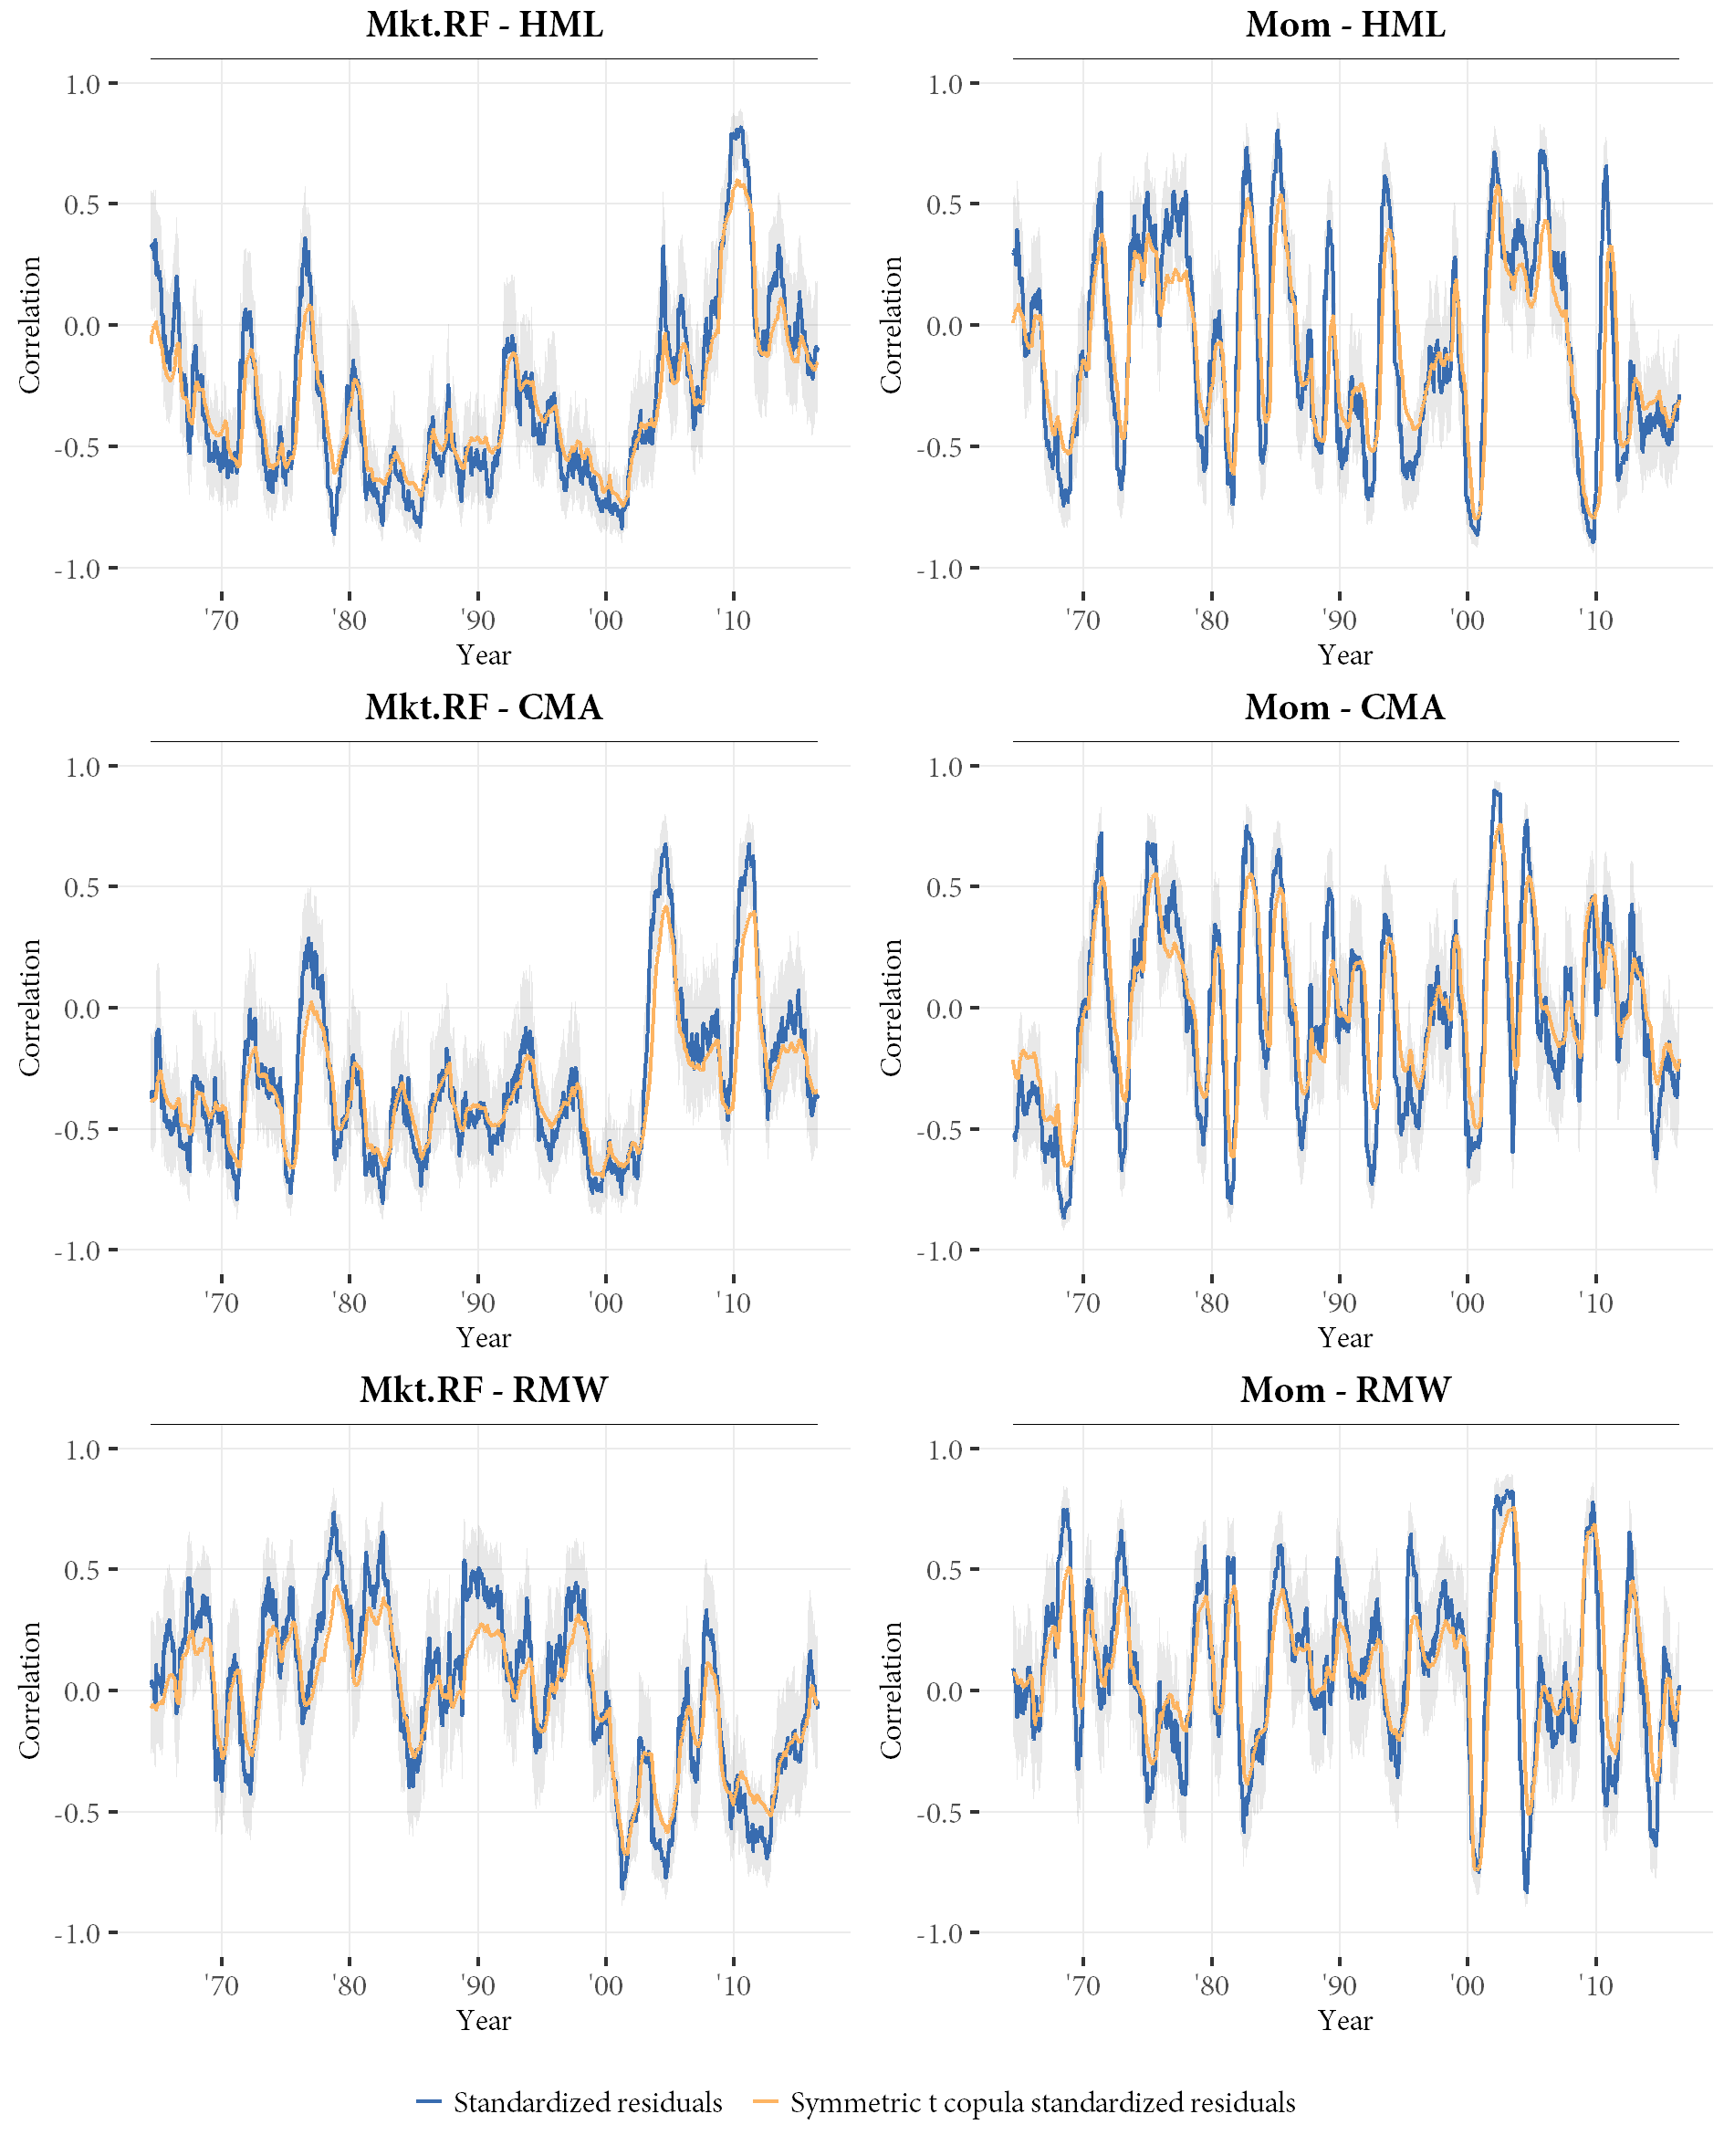
\includegraphics[width=\textwidth]{graphics/rolling_simulated1.png}
  \footnotesize
  \caption{Rolling correlations of standardized residuals from the dynamic copula}

  \begin{longcaption}
    Rolling correlations of the simulated dynamic symmetric \textit{t} copula compared to rolling correlations on ARMA-GARCH residuals. 95\% confidence bounds taking the ARMA-GARCH models as given. The simulated rolling correlations are based on 10,000 simulations each week. ARMA-GARCH models based on empirical weekly data 1963--2016.
  \end{longcaption}
  \label{fig:rolling_simulated}
\end{figure}
\begin{figure}[!ht]
  \ContinuedFloat
  \centering
  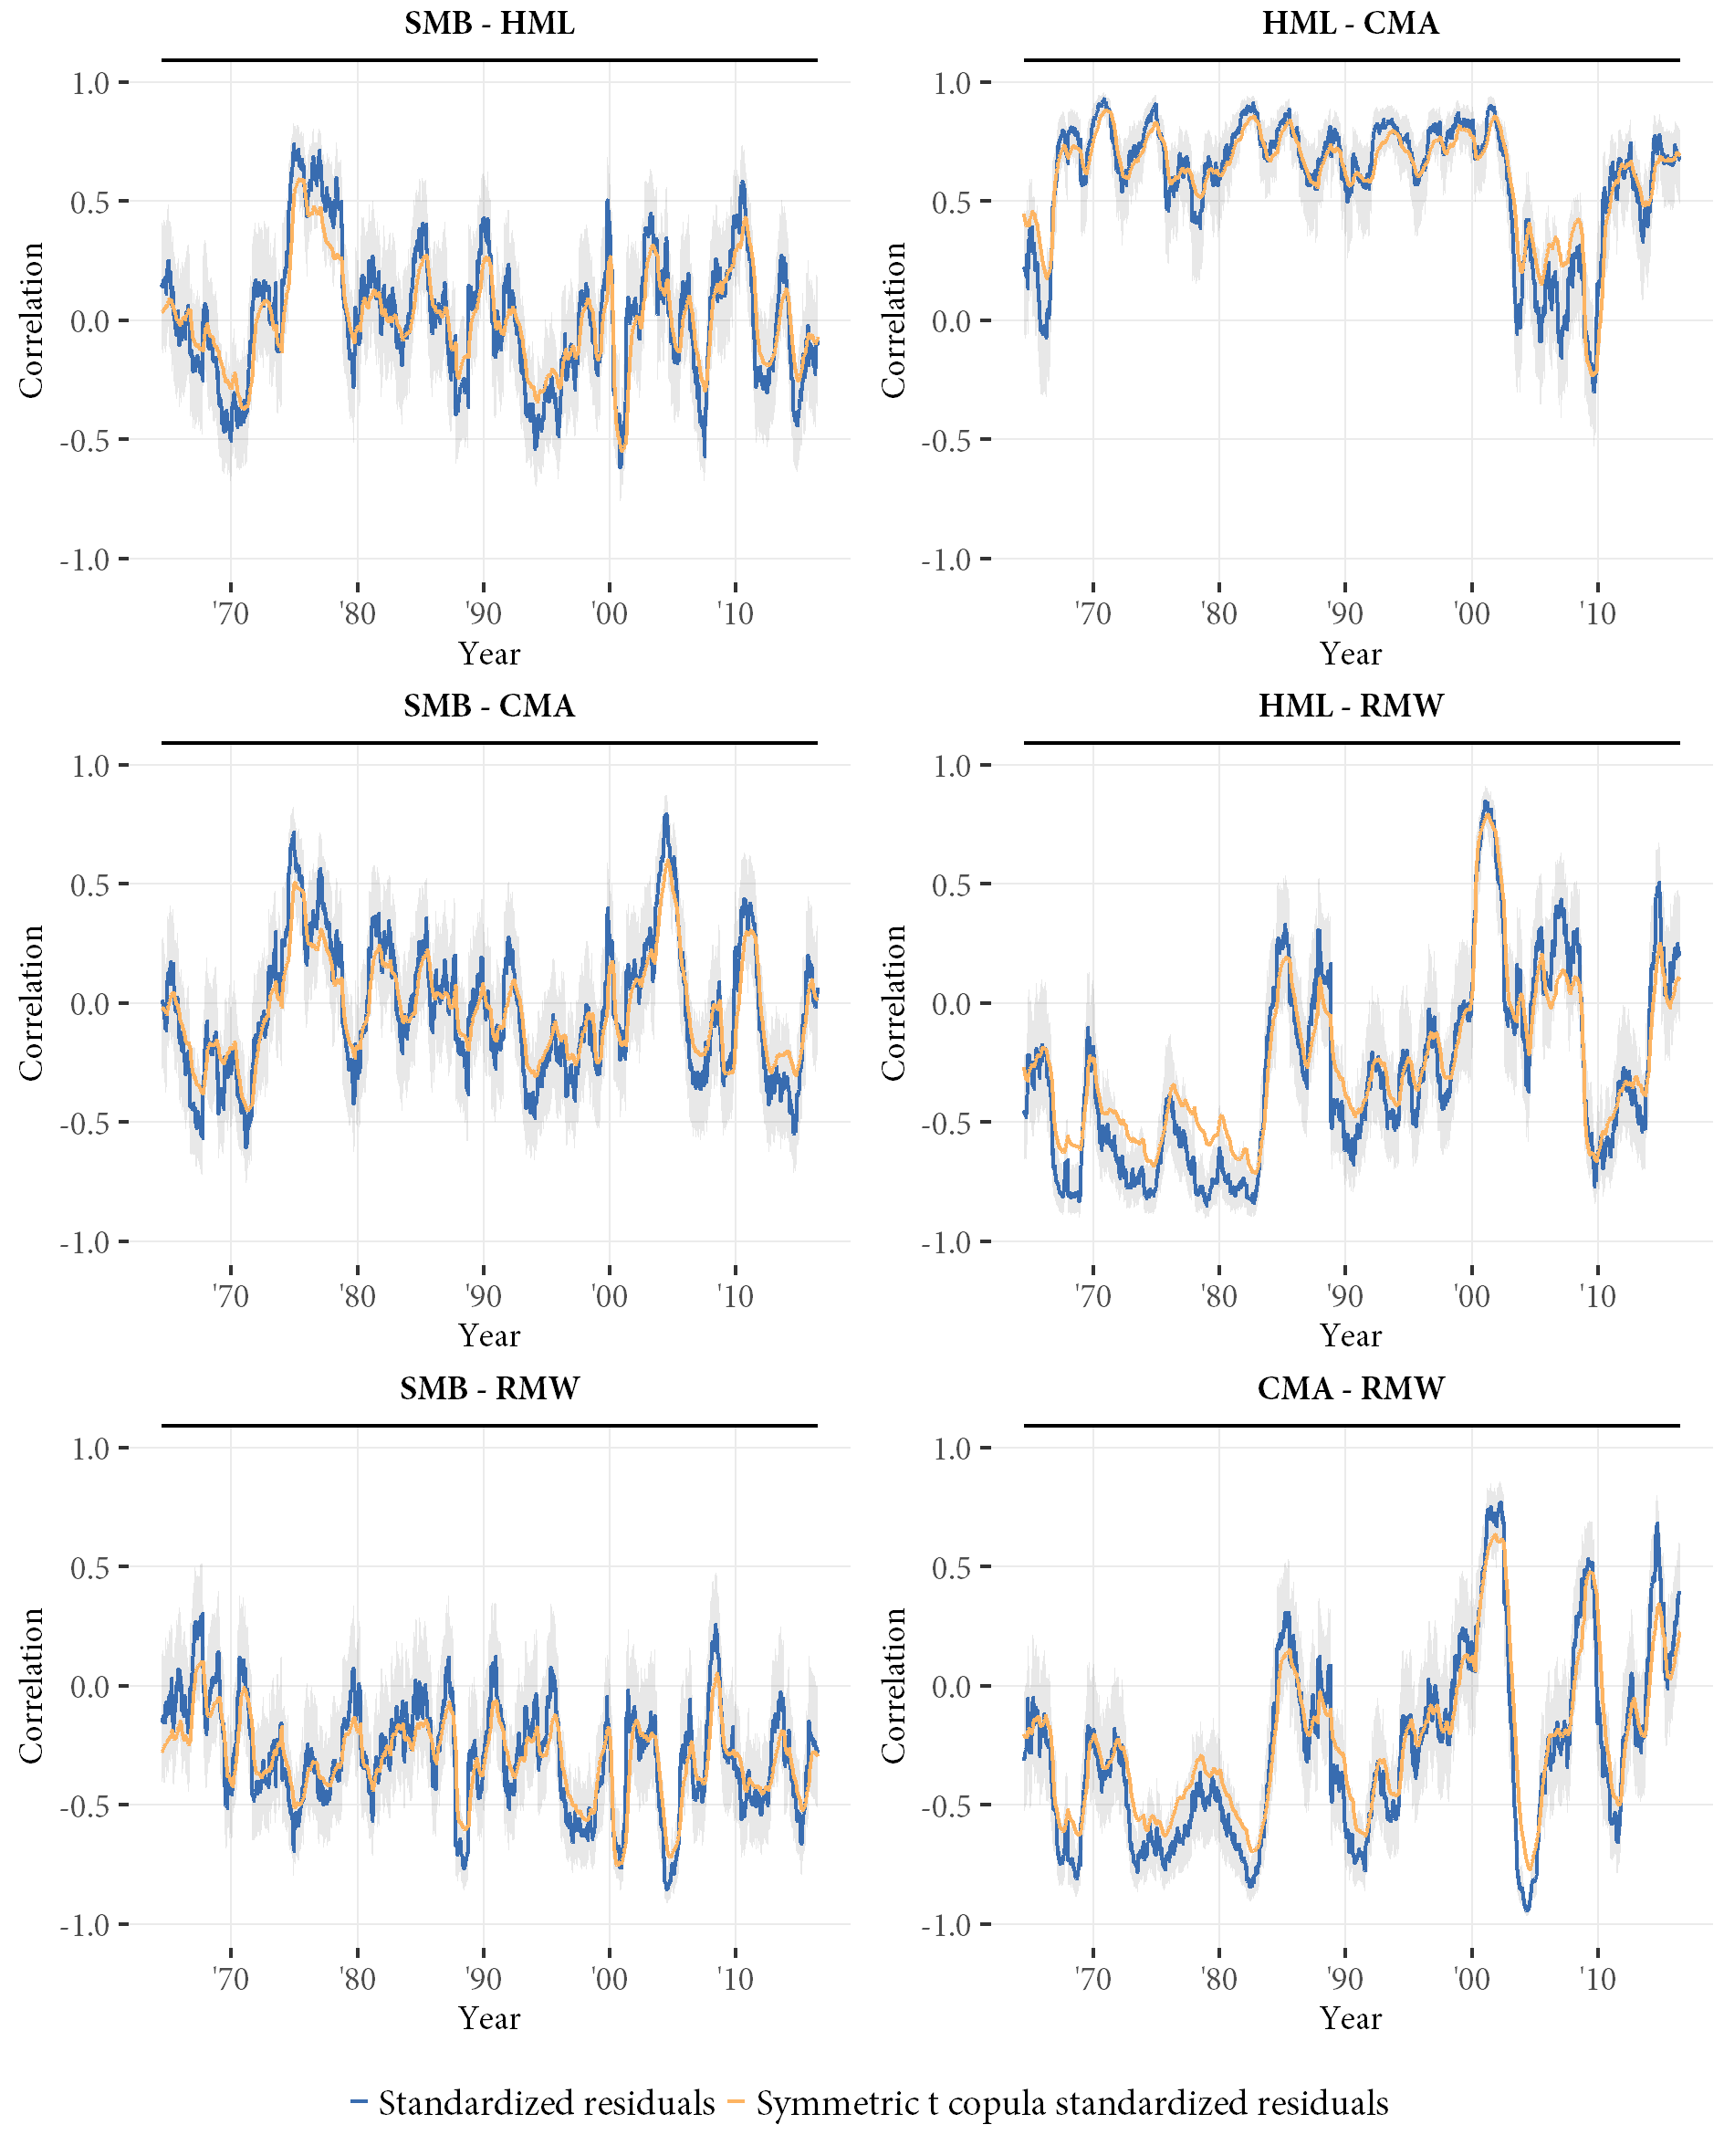
\includegraphics[width=\textwidth]{graphics/rolling_simulated2.png}
  \footnotesize
  \caption{Rolling correlations of standardized residuals from the dynamic copula (cont.)}
\end{figure}

While we do not get a perfect overlap, the copula model generates similar time-varying correlations. When there are large swings, however, the model does not always have enough amplitude. We conclude that the model captures the dynamic features well. % constant threshold corrs simulated, maybe also add robustness check of whether the model captures roll-corrs 

% section modeling_of_factor_returns (end)

%!TEX root = ../main.tex

\section{Optimizing factor allocations} % (fold)
\label{sec:optimizing_factor_allocations}

We now turn to the issue of optimizing factor allocations using our estimated model. Large money managers in the factor space generally advice against factor timing and use static strategies that are \emph{based} on equal-weighting -- a simple heuristic that has proven hard to beat out-of-sample. The managers do, however, blend the equal-weights approach with optimization routines, such as mean-variance and minimum-volatility, to arrive at static policy weights.\footnote{See i.a. \textcite{AQRSiren}, \textcite{BlackRock}, \textcite{MSCI} and \textcite{Robeco}.}

Our research question concerns the importance of HML given the discovery of RMW and CMA. Based on abnormal return regressions and the work on mean-variance portfolios in \textcite{HubermanKandel1987}, \textcite{FF2015} conjecture that the HML factor will not improve the mean-variance tangency portfolio when added to a portfolio of Mkt.RF, SMB, RMW and CMA. Differently put, this is equivalent to HML having a zero weight in mean-variance optimization. We evaluate this both based on static weights (based on sample estimates of expected returns and covariances) and dynamic weights (based on copula model estimates).

While dynamic weights may seem counter-intuitive at first, as investors use static allocations, we argue that the dynamic analysis is essential. Investors carry out real-time investing and can only use information up until the current date. We, on the other hand, evaluate the \emph{ex-post} merits of different asset universes (e.g. including and excluding HML), and use all available data to determine dynamic weights.

Moving beyond the mean-variance framework, because factor returns are not normal, the covariance matrix used in mean-variance optimization is not a full description of the dependency between factors.

This leads us to consider optimization using two techniques: Optimal Mean-Variance (MV) and optimal Conditional Diversification Benefit (CDB), which is a measure introduced by~\textcite{ChristoffersenErrunzaJacobLanglois2012}. The first optimization is a direct test of the conjecture in~\textcite{FF2015} that HML does not expand the mean-variance frontier. The second optimization is done to test the relative diversification benefit of different factors -- HML, CMA, RMW -- under non-normality.

CDB is based on the portfolio expected shortfall (ES), i.e. the expected loss in case the return realizes below its Value-at-Risk (VaR), and therefore concerns the properties of the lower tail of the portfolio distribution. This allows it to consider non-normalities in the return distribution.

The remainder of this section presents the construction of the CDB measure and presents the common optimization problem. Results of the optimizations are presented in the upcoming sections.

\subsection{Conditional Diversification Benefit} % (fold)
\label{sub:conditional_diversification_benefit}

This description of CDB follows~\textcite{ChristoffersenErrunzaJacobLanglois2012}. Define ES as the expected loss in some bottom percentile $q$:
\begin{align}
    \text{ES}_{i,t}^q(r_{i,t}) = -\mathbb{E}[r_{i,t} | r_{i,t} \leq F_{i,t}^{-1}(q)]
\end{align}
where $F_{i,t}^{-1}(q)$ is the inverse CDF of simple returns $r_{i,t}$ at $q$ (equivalent to the $q\%$ Value-at-Risk). 

The expected shortfall represents the expected loss when returns realize below the Value-at-Risk of the portfolio. Depending on the distribution at hand, the expected shortfall can be closer or further to the Value-at-Risk. Intuitively, if assets offer little diversification, then no combination of assets will reduce total portfolio risk; and ES will be higher. 

For a portfolio of assets with weights $w_t$, the portfolio ES $\text{ES}_t^q(w_t)$ has an upper bound equal to the weighted average of each asset's ES, corresponding to the case of no diversification~\autocite{Artzner1999}:
\begin{align}
  \overline{\text{ES}}_t^q(w_t) = \sum_{i=1}^N w_{i,t} \text{ES}_{i,t}^q(r_{i,t})
\end{align}
A lower bound on portfolio ES is given by the portfolio's Value-at-Risk ($-F_{t}^{-1}(w_t, q)$):
\begin{align}
  \underline{\text{ES}}_t^q(w_t) = -F_{t}^{-1}(w_t, q)
\end{align}
CDB is defined as the portfolio's ES scaled by its lower and upper bounds:
\begin{align}
  \text{CDB}_t^q(w_t) = \frac{\overline{\text{ES}}_t^q(w_t) - \text{ES}_t^q(w_t)}{\overline{\text{ES}}_t^q(w_t) - \underline{\text{ES}}_t^q(w_t)}
\end{align}
CDB is a number between zero and one (we report CDB scaled to 0--100) and thus measures how close to its Value-at-Risk the expected shortfall of a portfolio gets (we report CDB scaled by 100). Note that the level of expected return does not enter into the measure -- CDB only measures how ``useful'' a group of assets are for eliminating risk.

% subsection conditional_diversification_benefit (end)

\subsection{Optimization Problem} % (fold)
\label{sub:optimization_problem}

Each week, we choose portfolio weights to maximize the Sharpe Ratio (SR) in the mean-variance case, and CDB in the CDB case. We impose two restrictions on our optimization problem. First, all factor weights must be positive. This reduces the problem with extreme weights, seen in the unconstrained optimization problem, and reflects a view that an investor will not bet against factors that have generated a history of positive premia. Second, factor weights must sum to unity, i.e. fully invested across factors. In light of~\textcite{Asness2015}, we consider portfolios with and without momentum (five- and six-factor portfolios, respectively) and how portfolio weights change when replacing HML with CMA and vice versa.

Together, these restrictions make the maximized Sharpe Ratio reflect tangency weights subject to a constraint of no negative weights. Due to the restrictions, the standard analytical solution to the mean-variance problem is not equal to the tangency portfolio. Similarly, no analytical solution exists for optimizing CDB. Hence, we performa a numerical optimization where we choose weights $w_t$ to maximize the objective function $\Omega_t(w_t)$ subject to the above restrictions:
\begin{align}
  \arg\!\max_{w_t} \Omega_t(w_t)
    &&\text{\quad s.t.\quad} & \sum_{i=1}^N w_{i,t} = 1 \\
    &&                       & w_{i,t} \ge 0 \notag
\end{align}
For the MV case, the objective function is the one-week Sharpe Ratio (SR):
\begin{align}
  \Omega_t(w_t) = \frac{w_t^\top \mathbb{E}_t[r_{t+1}]}{\sqrt{w_t^\top \mathbb{E}_t[\Sigma_{t+1}] w_t}}
\end{align}
$\mathbb{E}_t[r_{t+1}]$ is the conditional one-step-ahead expected factor return and $\mathbb{E}_t[\Sigma_{t+1}]$ is the conditional one-step-ahead variance-covariance matrix. 

For the CDB case, the objective function is the one-week CDB:
\begin{align}
  \Omega_t(w_t) = \text{CDB}_t^q(w_t)
\end{align}
Each week, we perform MV and CDB optimization using simulated distributions from our fully estimated dynamic copula model. Each week, we simulate $10\,000$ returns from the estimated copula model and use those outcomes as the conditional distribution of factor returns. We also perform MV optimization based on sample means and covariances, in which case $\mathbb{E}_t[r_{t+1}]$ and $\mathbb{E}_t[\Sigma_{t+1}]$ are constant and equal to the full-sample estimates.

% subsection optimization_problem (end)

% section optimizing_factor_allocations (end)

%!TEX root = ../main.tex

\section{Results from mean-variance optimization} % (fold)
\label{sec:mean_variance}

In \autoref{fig:mv_optimal_5}, we present the optimized weights over time in the five-factor universe (four-factor when one factor is excluded). The left hand column presents weights of factors when we consider the inclusion and exclusion of HML, while the right hand column presents weights of factors when CMA is included and excluded. The dynamic weights are based on one-week-ahead forecasts from the copula model, while the static lines represent the weights based on sample estimators of the mean-variance inputs.

Accompanying the graph, \autoref{tab:mv_model} presents average MV optimal weights based on dynamic inputs of expected returns and covariances from the copula model. This table also gives average weight differences between models, as well as a number of performance measures that are based on the realized returns. The CDB statistic is based on MV optimal weights and uses the copula model as the distribution of returns. Please note that all performance measures are calculated in-sample and are not indicative of out-of-sample investing based on a copula model; they should be interpreted only in relative terms, in order to determine how much a portfolio is impacted by the exclusion of a factor.\footnote{A similar table of performance measures and average weight differences using in-sample sample estimators of expected returns and covariances is found in~\autoref{tab:mw_mv_sample} (\autoref{app:supplementary}).}

\begin{figure}[p]
  \centering
  \footnotesize
  \begin{subfigure}{0.45\textwidth}
    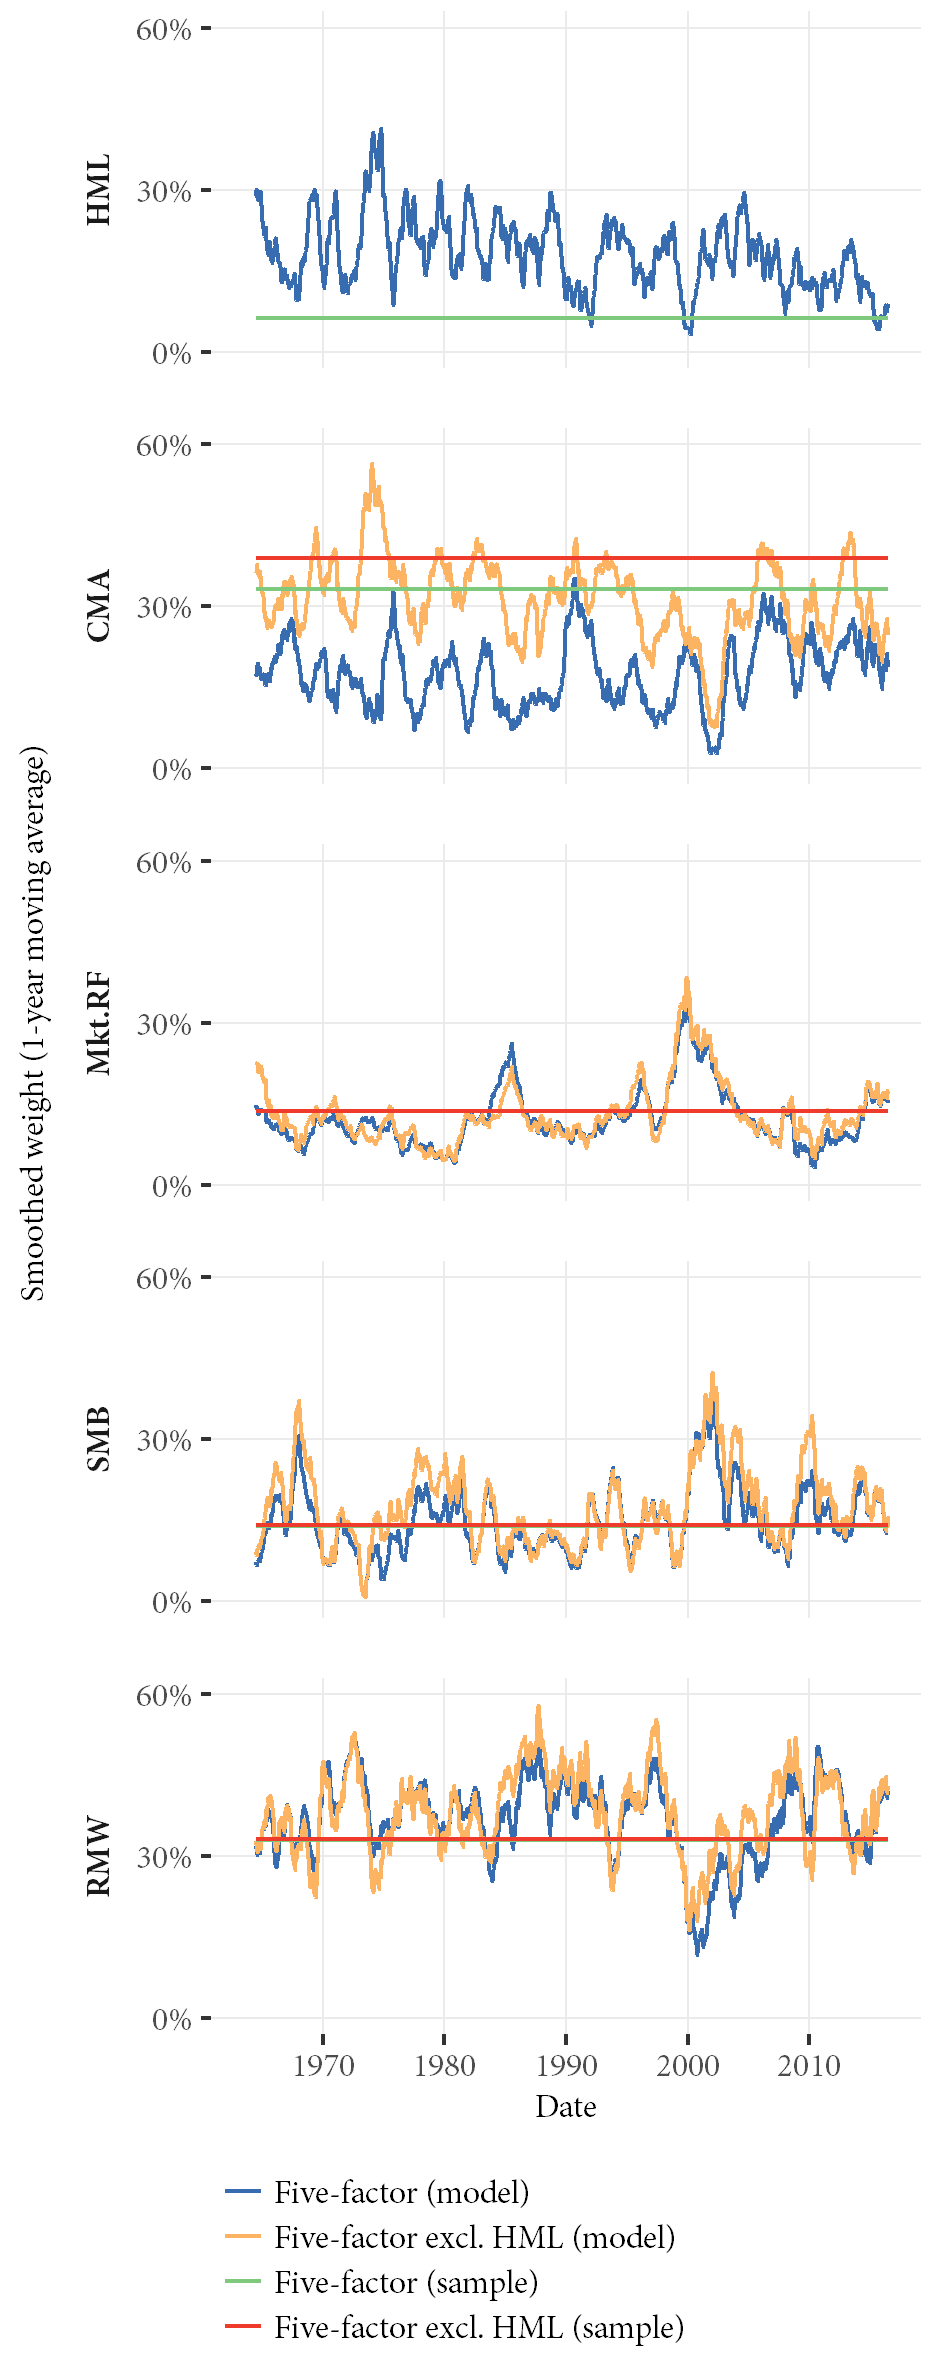
\includegraphics[width=\textwidth]{graphics/weights/main_Weights_MV_5F_EXCL_HML_5F.png}
    \caption{Excluding HML}
  \end{subfigure}
  ~
  \begin{subfigure}{0.45\textwidth}
    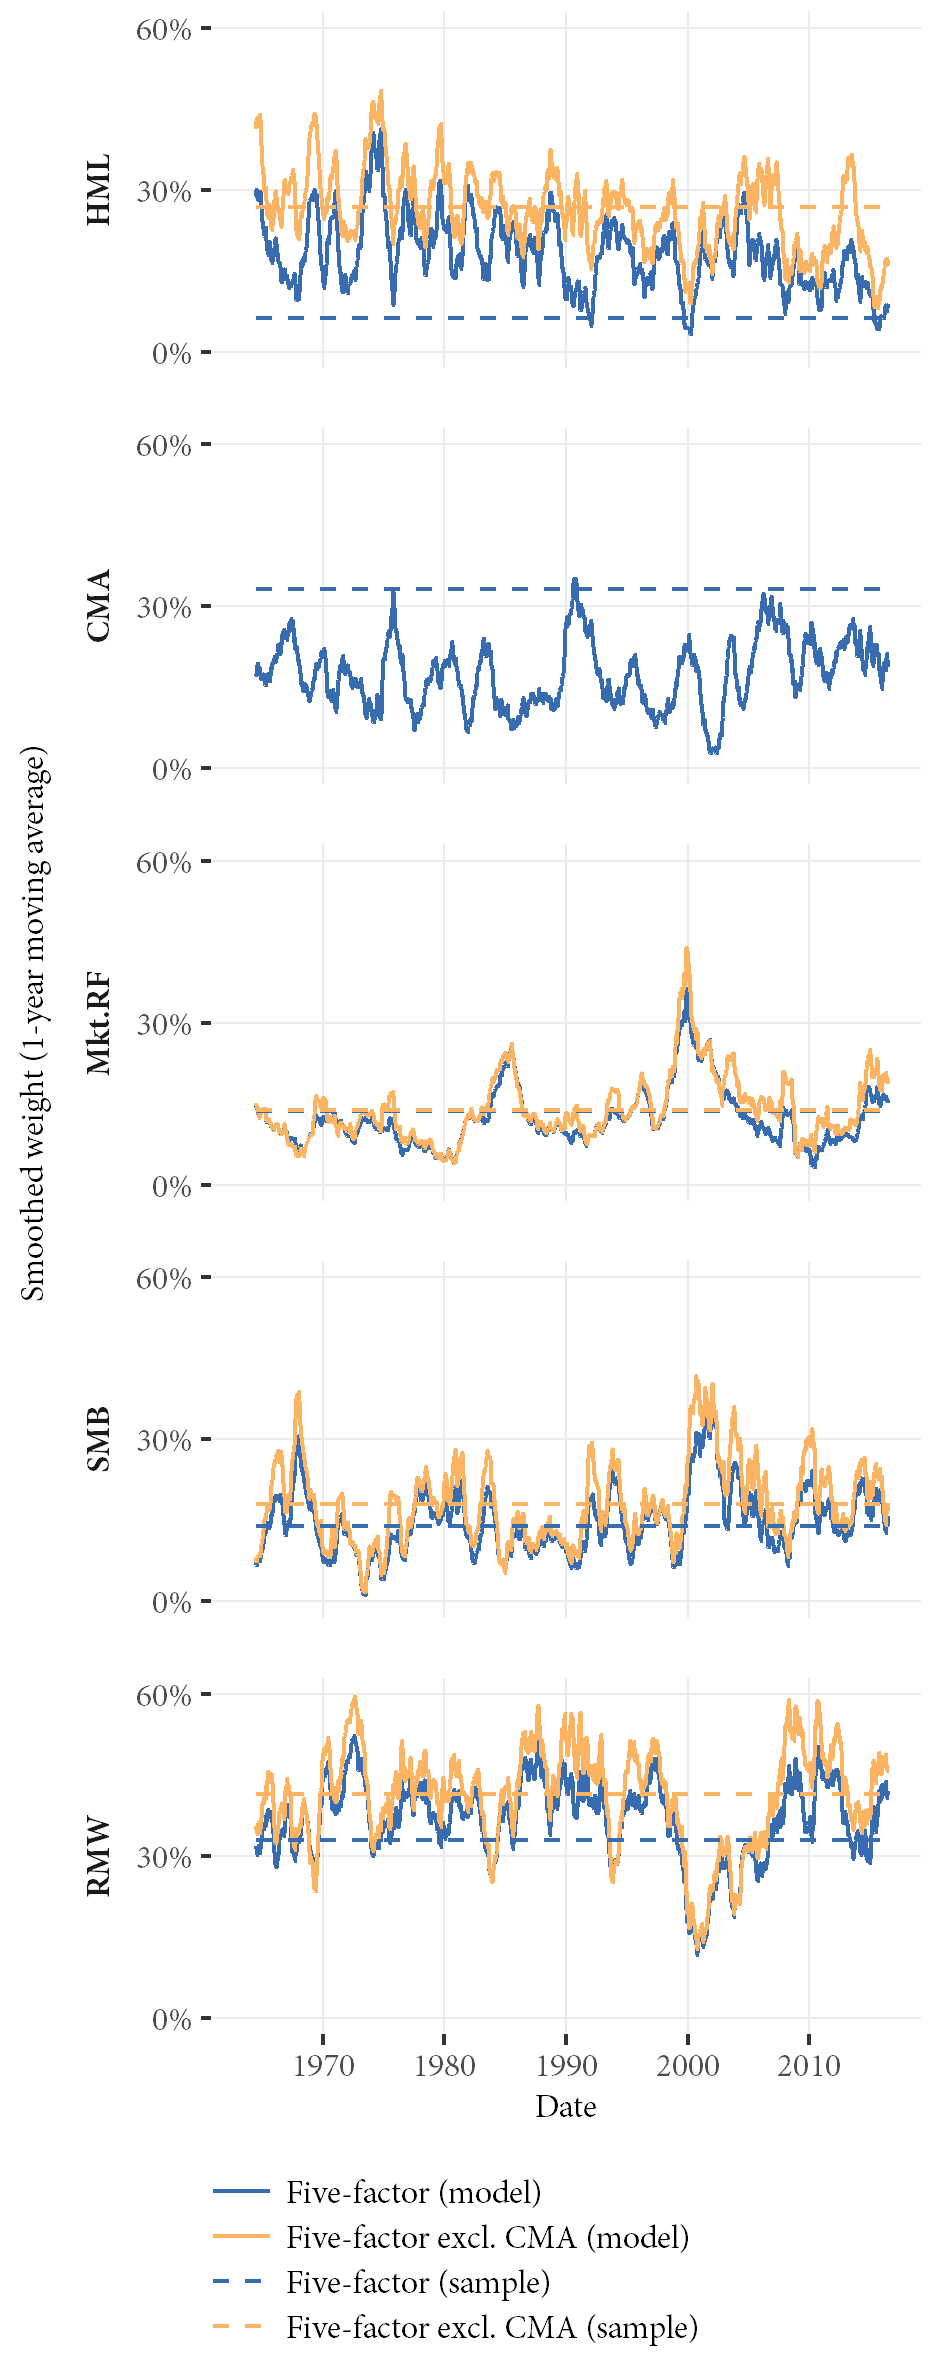
\includegraphics[width=\textwidth]{graphics/weights/main_Weights_MV_5F_EXCL_CMA_5F.png}
    \caption{Excluding CMA}
  \end{subfigure}  
  \caption{Mean-variance optimal weights with five factors}
  \label{fig:mv_optimal_5}

  \begin{longcaption}
    Smoothed as 1-year moving averages for better legibility. Optimization constrained to fully invested portfolios with non-negative weights. Left hand panel including and excluding HML, right hand including and excluding CMA. Based on one-week-ahead forecasts from the dynamic symmetric \emph{t} copula model 1963--2016.
  \end{longcaption}
\end{figure}
\begin{figure}[p]
  \ContinuedFloat
  \centering
  \begin{subfigure}{0.45\textwidth}
    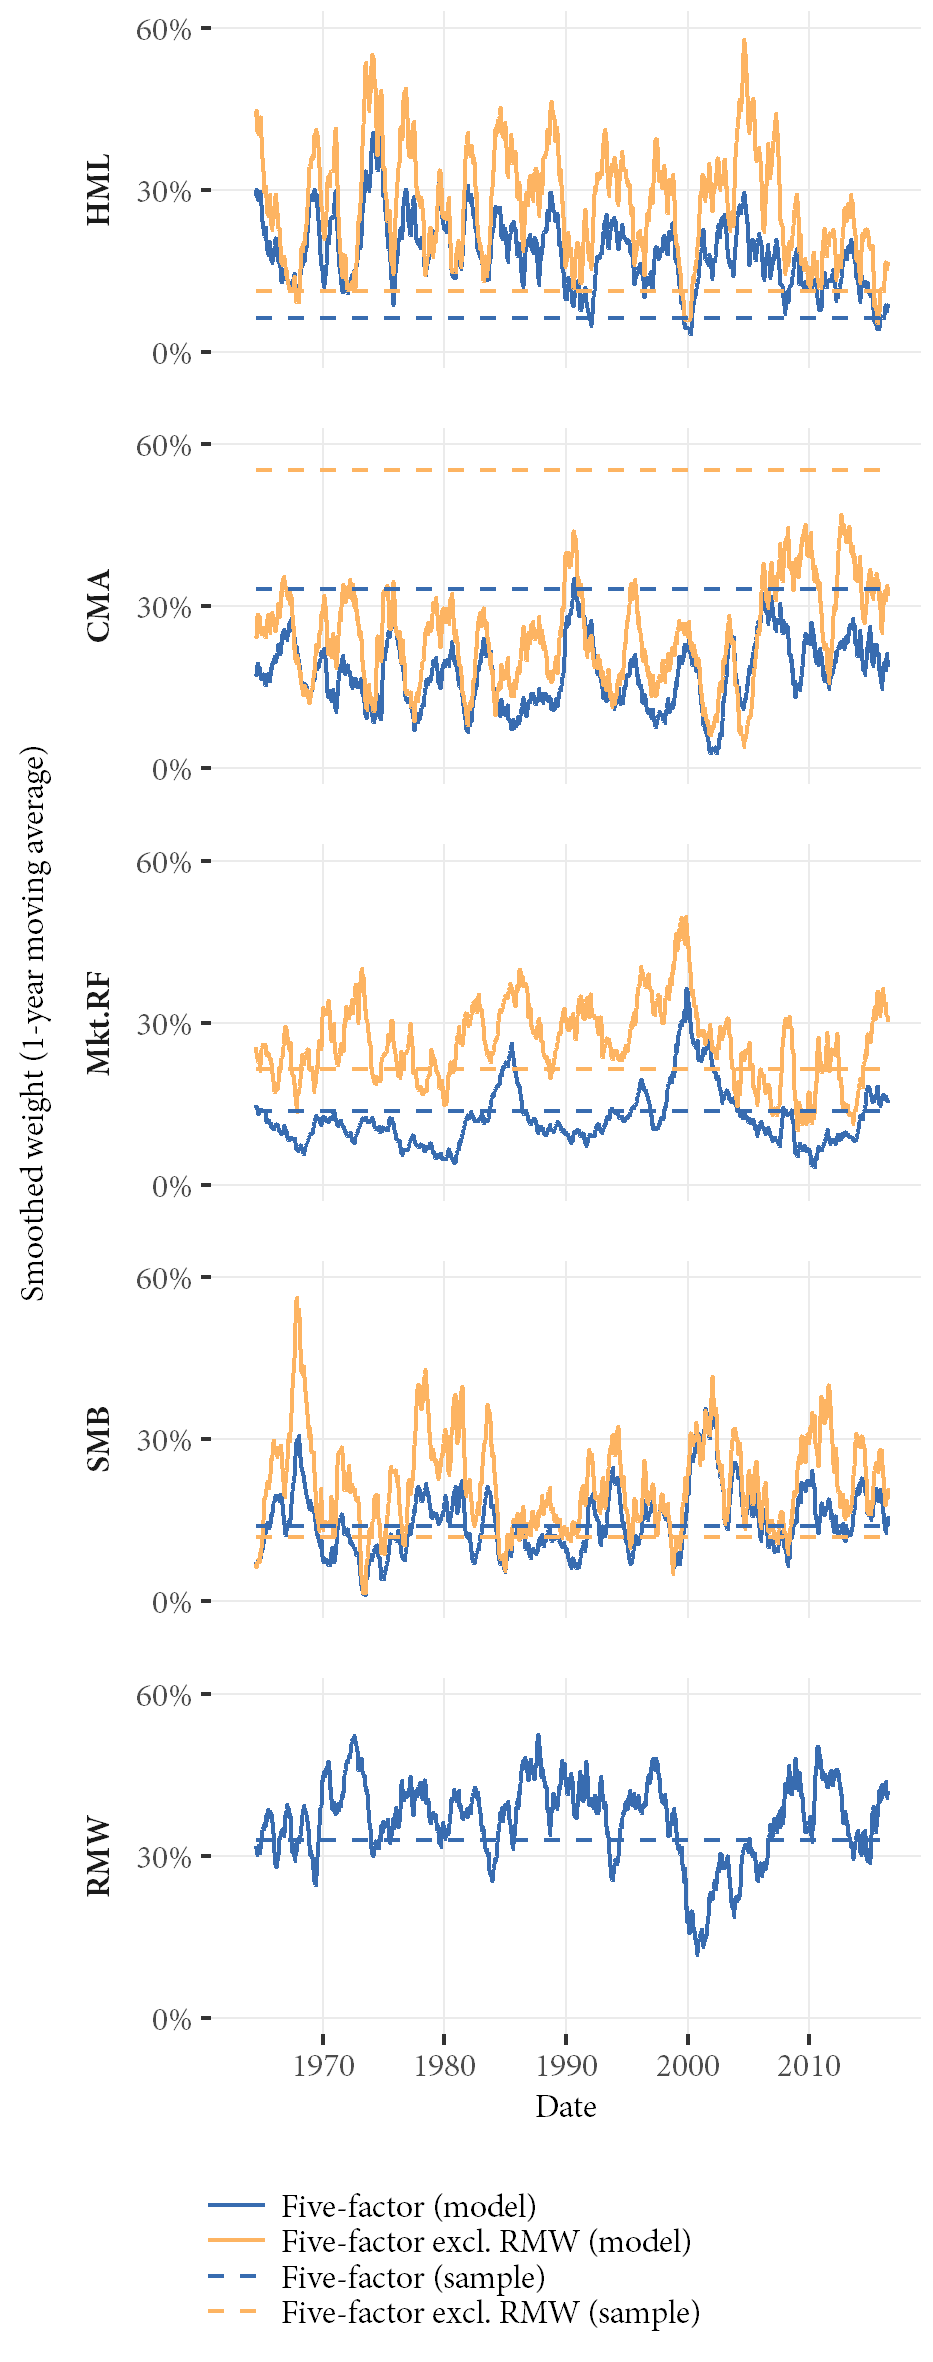
\includegraphics[width=\textwidth]{graphics/weights/main_Weights_MV_5F_5F_EXCL_RMW.png}
    \caption{Excluding RMW}
  \end{subfigure}  
  \footnotesize
  \caption{Mean-variance optimal weights with five factors (cont.)}
\end{figure}

We begin by examining the left column of plots in \autoref{fig:mv_optimal_5} that includes and excludes HML in the five-factor universe. First, we note that the weight of HML is clearly not zero when introduced in the investible universe. This appears to be the case for both the sample estimate of means and covariances, as well as the dynamic estimates from the copula model. Both inputs suggest that HML does in fact improve the tangency portfolio, as the optimal portfolio has a positive weight on the factor. The inclusion of HML leads to an increase in realized SR, which goes from 1.48 to 1.64. Furthermore, including HML leads to a less risky portfolio, with slightly lower average VaR and average ES and a higher degree of tail diversification, as measured by CDB (see \autoref{tab:mv_model}).

Although we impose the additional restriction of no negative weights, this finding does stand in contrast to the conjecture in \textcite{FF2015} that HML should not improve the tangency portfolio. While the unconstrained tangency portfolio may or may not include HML, the simple restriction of no negative weights makes HML an important part of the optimal portfolio. However, we notice that this is less clear if we do not use dynamic inputs. For the full five-factor model, static sample estimators result in a lower allocation to HML (6.2\%) than the dynamic inputs from the copula (average 18.2\%), and a much smaller difference in realized SR, which goes from 1.25 to 1.27 (see \autoref{tab:mw_mv_sample} (\autoref{app:supplementary}) for sample results).

Second, from the left panel of \autoref{fig:mv_optimal_5}, we note that the dynamic weight of HML seems to be highly similar to the decrease in weight in CMA, while all the remaining factors seem to stay very close to their original weights when moving to the full five-factor model. In other words, the weight that is attributed to HML is drawn nearly directly from the weight of CMA, in each period. Our interpretation is that in a five-factor model excluding HML (effectively a four-factor model), CMA proxies for HML, which is why CMA absorbs nearly all the weight. HML also seems to proxy for CMA to a lesser extent, as shown by the right hand column of plots in \autoref{fig:mv_optimal_5}, which include and exclude CMA. When CMA is included, the weight of HML is lowered, but so are the weights of SMB and RMW. The proxying behavior of HML and CMA is expected, as the factors are highly correlated and zero-cost portfolio regressions in this thesis (\autoref{fig:abnormal}), as well as in \textcite{FF2015} and \textcite{Asness2015}, indicate that the main explanatory variable for HML is CMA, and vice versa.

Third, from the third panel of \autoref{fig:mv_optimal_5}, presented on a separate page, we find that among the two newly introduced factors CMA and RMW, the latter seems to have a much more substantial impact on the mean-variance portfolio. RMW receives weights of approx. 35\% in the five-factor model, which is nearly twice the allocation of any other factor. Furthermore, the inclusion of RMW leads to a large improvement of portfolio performance measures. For dynamic weights in the five-factor model, RMW makes the realized SR go from 1.28 to 1.64. At the same time, RMW leads to large decreases in the average VaR and average ES risk measures, both of which are nearly halved when RMW is included. This highlights the large benefits of including the RMW strategy in a factor portfolio, which are expected due to RMW's low or negative factor loadings in the zero-cost portfolio regressions (see \autoref{sec:alpha_reg}).

We now move on to the six-factor model universe (effectively five-factor models when one factor is excluded), with weights in \autoref{fig:mv_optimal_6} and figures in the right hand panel of \autoref{tab:mv_model}. As the optimal weights and performance results are in general qualitatively similar to the five-factor model, we will only comment on key changes.

In the expanded universe, Sharpe Ratios are generally very high, regardless of whether a factor is excluded. Surprisingly, the highest SR is realized when CMA is excluded. However, the difference is small and we do not put too much emphasis on this interpretation. Another notable change is that the allocation to HML based on static sample inputs is now higher (13.2\% compared to 6.2\%), which could be due to the clearer recognition of momentum differences between HML and CMA firms as Mom is included (cf. the discussion on zero-cost regressions in \autoref{sec:alpha_reg}). 

In summary, we examine weights and portfolio performance measures for optimal MV portfolios and find no reason to believe that mean-variance investing in the HML factor is dead or fully subsumed by the remaining factors, as the optimal portfolios include HML and have higher realized Sharpe Ratios, as well as lower realized risk measures. We also find that the inclusion of RMW is substantially more important, and leads to a large weight allocation to the factor as well as a substantial improvement on all performance measures.

\begin{figure}[p]
  \centering
  \footnotesize

  \begin{subfigure}{0.45\textwidth}

    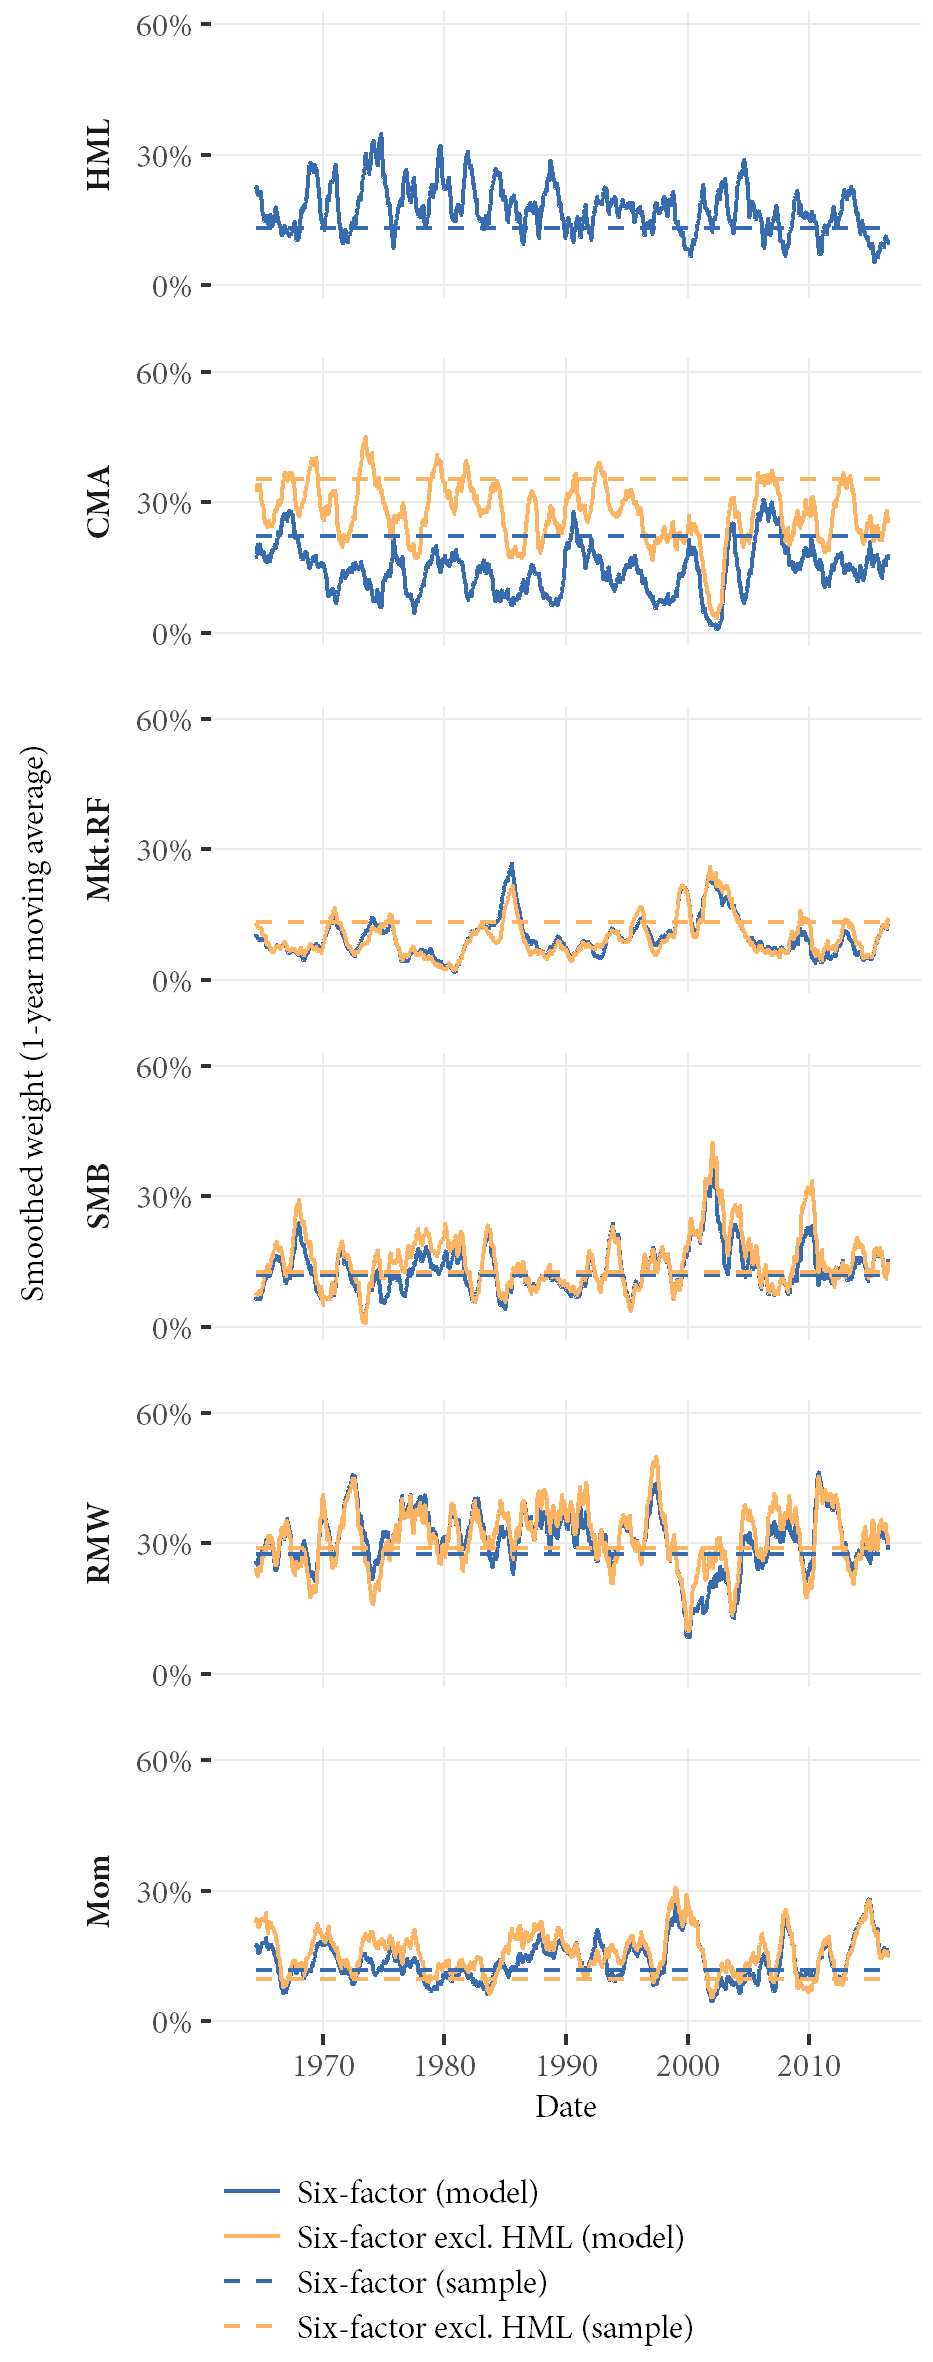
\includegraphics[width=\textwidth]{graphics/weights/main_Weights_MV_6F_EXCL_HML_6F.png}
    \caption{Excluding HML}
  \end{subfigure}
  ~
  \begin{subfigure}{0.45\textwidth}
    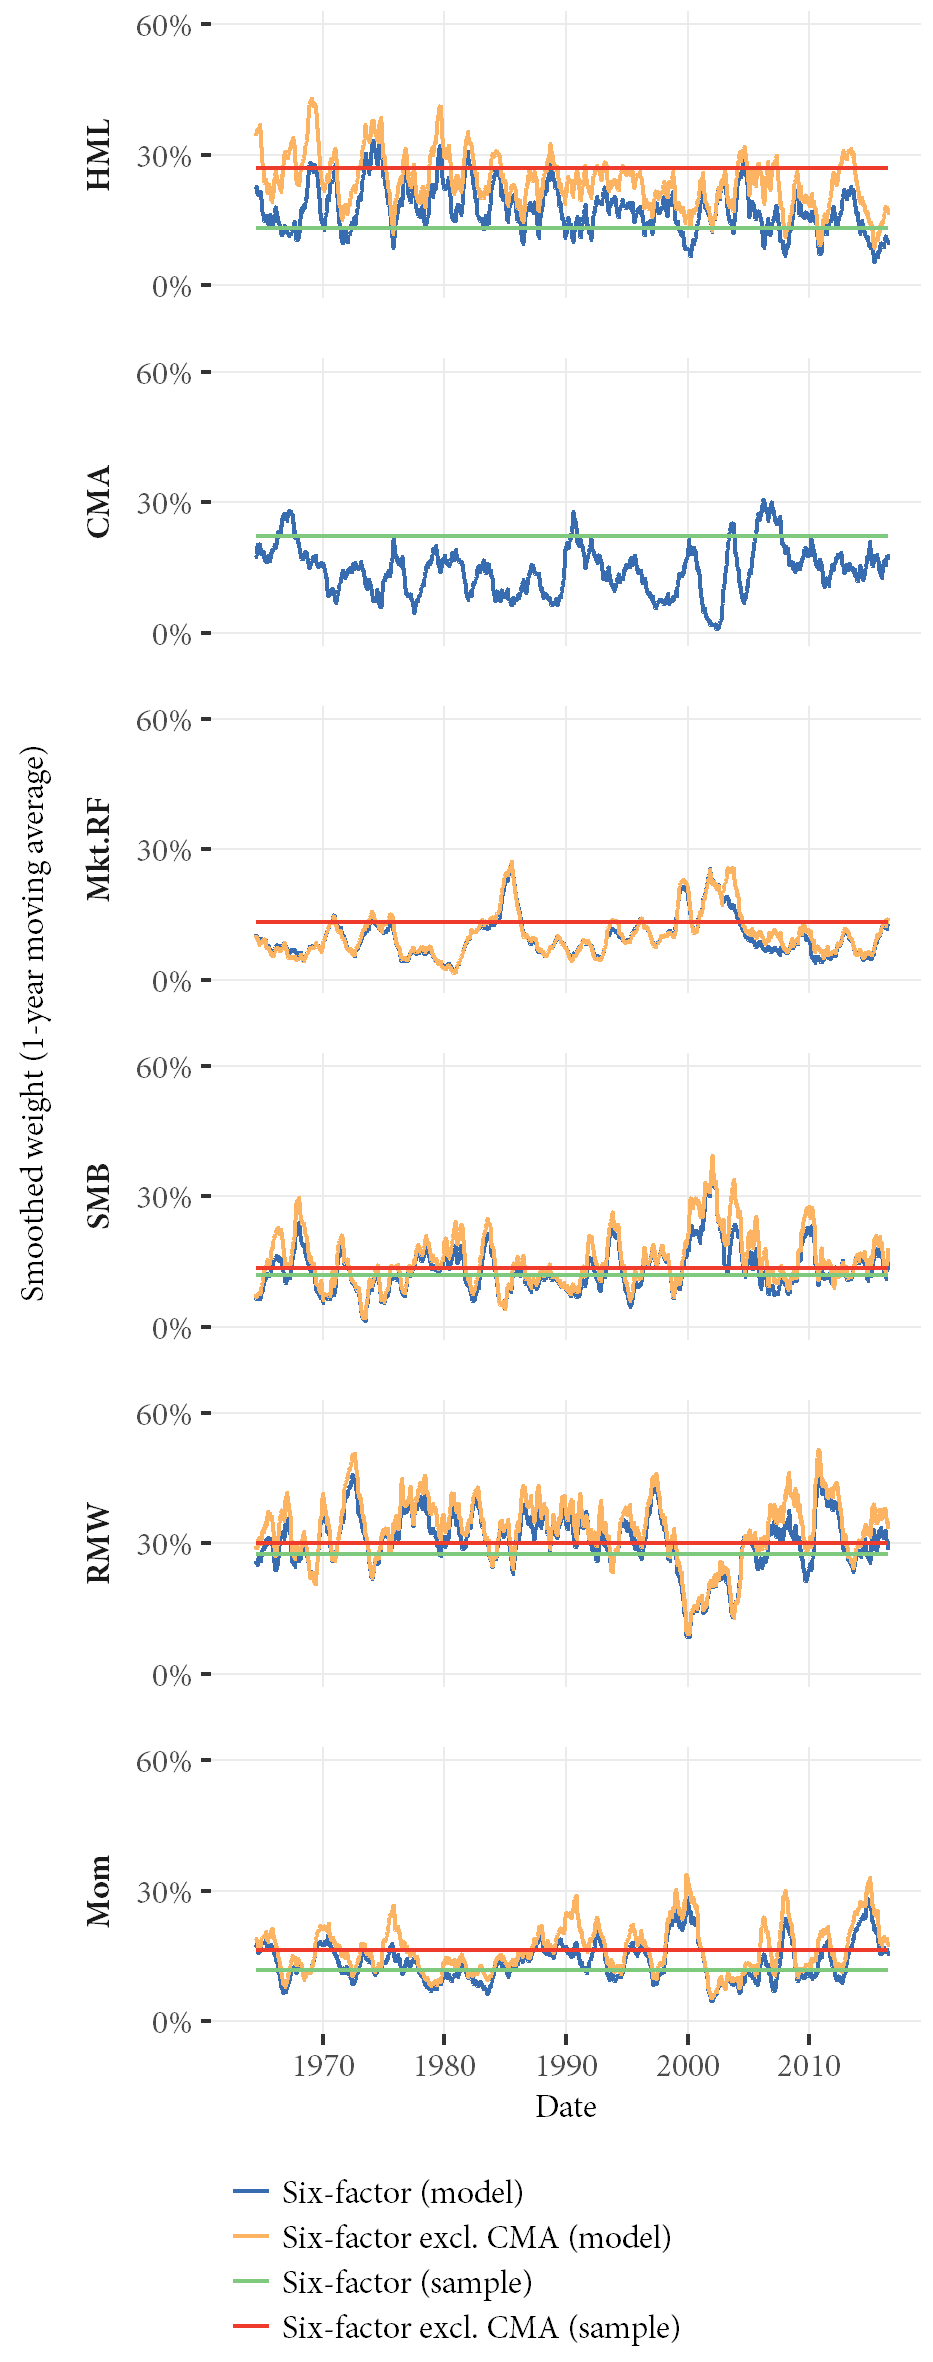
\includegraphics[width=\textwidth]{graphics/weights/main_Weights_MV_6F_EXCL_CMA_6F.png}
    \caption{Excluding CMA}
  \end{subfigure}
  \caption{Mean-variance optimal weights with six factors}

  \begin{longcaption}
    Smoothed as 1-year moving averages for better legibility. Optimization constrained to fully invested portfolios with non-negative weights. Left hand panel including and excluding HML, right hand including and excluding CMA. Based on one-week-ahead forecasts from the dynamic symmetric \emph{t} copula model 1963--2016.
  \end{longcaption}
\end{figure}

\begin{figure}[p]
  \ContinuedFloat
  \centering
  \begin{subfigure}{0.45\textwidth}
    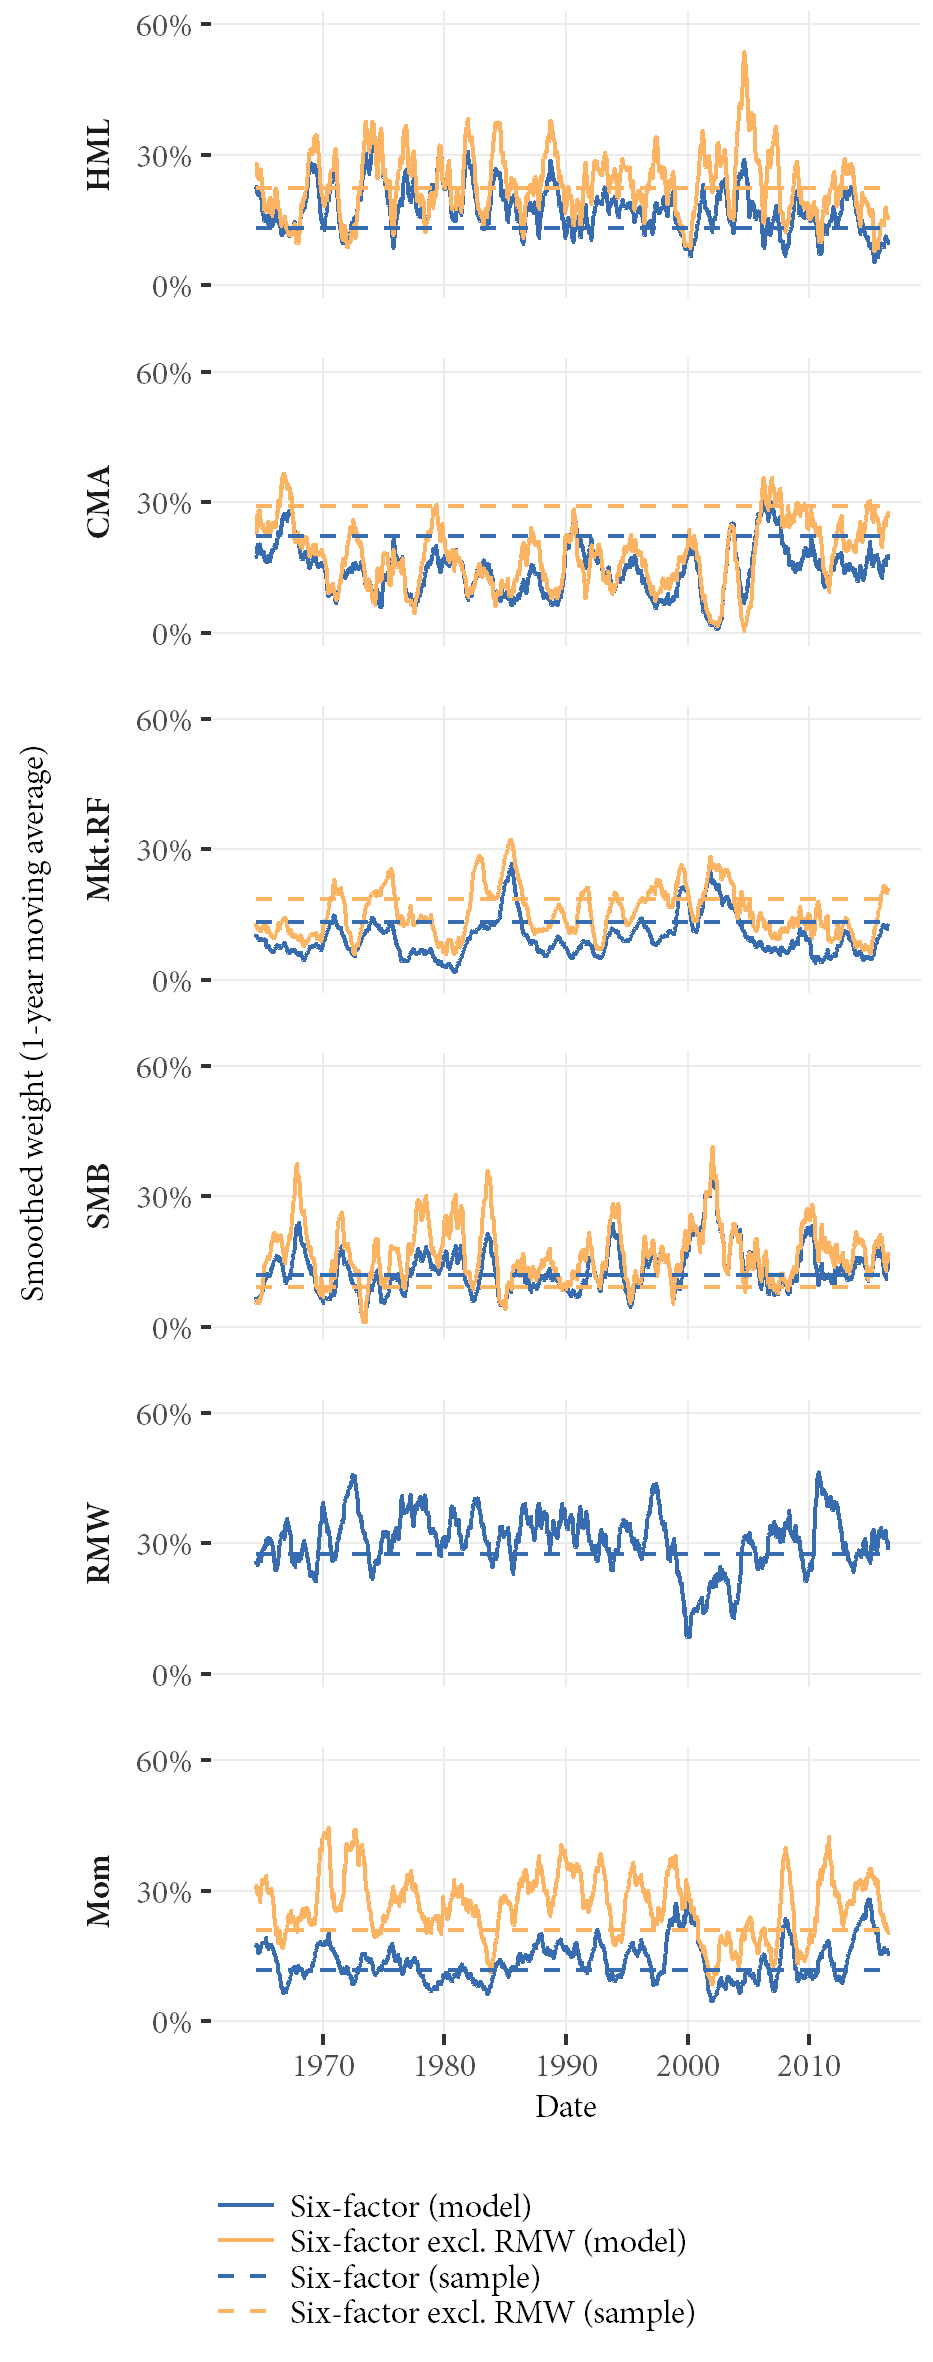
\includegraphics[width=\textwidth]{graphics/weights/main_Weights_MV_6F_6F_EXCL_RMW.png}
    \caption{Excluding RMW}
  \end{subfigure}
  \footnotesize
  \caption{Mean-variance optimal weights with six factors (cont.)}
  \label{fig:mv_optimal_6}
\end{figure}

%!TEX root = ../../main.tex

\begin{table}
  \centering
  \footnotesize
  \renewcommand{\arraystretch}{1.2}

  \caption{Mean-Variance Optimization with Dynamic Copula Model (1963--2016)}

  \begin{longcaption}
    Lorem ipsum dolor sit amet, consectetur adipisicing elit, sed do eiusmod
    tempor incididunt ut labore et dolore magna aliqua. Ut enim ad minim veniam,
    quis nostrud exercitation ullamco laboris nisi ut aliquip ex ea commodo
    consequat. Duis aute irure dolor in reprehenderit in voluptate velit esse
    cillum dolore eu fugiat nulla pariatur. Excepteur sint occaecat cupidatat non
    proident, sunt in culpa qui officia deserunt mollit anim id est laborum.
  \end{longcaption}

  \label{tab:mv_model}

  \begin{tabularx}{\textwidth}{@{} l dddd X dddd @{}}
    \toprule
    &
      \multicolumn{4}{c}{Five Factors} &&
      \multicolumn{4}{c}{Six Factors} \\
    \cmidrule{2-5}
    \cmidrule{7-10}
    &
      \multirow{2}{*}{All} &
      \multicolumn{1}{c}{Excl} &
      \multicolumn{1}{c}{Excl} &
      \multicolumn{1}{c}{Excl} & &
      \multirow{2}{*}{All} &
      \multicolumn{1}{c}{Excl} &
      \multicolumn{1}{c}{Excl} &
      \multicolumn{1}{c}{Excl} \\
    &
      &
      \multicolumn{1}{c}{HML} &
      \multicolumn{1}{c}{CMA} &
      \multicolumn{1}{c}{RMW} &&
      &
      \multicolumn{1}{c}{HML} &
      \multicolumn{1}{c}{CMA} &
      \multicolumn{1}{c}{RMW} \\
    \midrule
    \multicolumn{1}{@{}l}{\textbf{Average weights}} \\
    Mkt.RF & 12.4 & 13.2 & 14.2 & 26.4 & & 9.9  & 9.9  & 10.4 & 15.5 \\
    SMB    & 15.0 & 17.4 & 18.3 & 21.8 & & 13.4 & 15.3 & 15.6 & 16.8 \\
    HML    & 18.2 &      & 26.3 & 27.2 & & 17.6 &      & 24.1 & 23.1 \\
    CMA    & 17.6 & 31.4 &      & 24.6 & & 14.6 & 27.5 &      & 17.8 \\
    RMW    & 36.8 & 38.0 & 41.2 &      & & 30.6 & 31.4 & 33.3 & \\
    Mom    &      &      &      &      & & 13.9 & 15.9 & 16.6 & 26.8 \\
    \midrule
    \multicolumn{1}{@{}l}{\textbf{Difference weights}} \\
    Mkt.RF & & 0.8   & 1.8   & 14.0  & & & 0.1   & 0.6   & 5.7 \\
    SMB    & & 2.4   & 3.3   & 6.8   & & & 1.9   & 2.2   & 3.4 \\
    HML    & & -18.2 & 8.1   & 9.0   & & & -17.6 & 6.5   & 5.5 \\
    CMA    & & 13.8  & -17.6 & 7.0   & & & 12.9  & -14.6 & 3.2 \\
    RMW    & & 1.2   & 4.4   & -36.8 & & & 0.8   & 2.7   & -30.6     \\
    Mom    & &       &       &       & & & 2.0   & 2.7   & 12.8 \\
    \midrule
    \multicolumn{1}{@{}l}{\textbf{Performance}} \\
    Mean (\%)      & 6.48  & 6.42  & 7.28  & 8.88  & & 7.18  & 7.34  & 8.12  & 9.94 \\
    SD (\%)        & 3.95  & 4.34  & 4.72  & 6.93  & & 4.05  & 4.39  & 4.49  & 5.83 \\
    Skewness       & 0.20  & -0.22 & -0.41 & -0.20 & & -1.46 & -1.46 & -1.09 & -0.55 \\
    Kurtosis       & 13.68 & 16.13 & 15.44 & 10.36 & & 29.59 & 27.25 & 21.07 & 13.11 \\
    SR             & 1.64  & 1.48  & 1.54  & 1.28  & & 1.77  & 1.67  & 1.81  & 1.70 \\
    MDD (\%)       & 11.03 & 11.89 & 13.18 & 25.32 & & 10.48 & 11.92 & 11.19 & 13.10 \\
    Avg. VaR  (\%) & 0.59  & 0.68  & 0.73  & 1.14  & & 0.56  & 0.64  & 0.66  & 0.93 \\
    Avg. ES  (\%)  & 0.83  & 0.94  & 1.02  & 1.58  & & 0.79  & 0.90  & 0.93  & 1.31 \\
    Avg. CDB       & 0.83  & 0.79  & 0.78  & 0.68  & & 0.85  & 0.81  & 0.82  & 0.75 \\
    \midrule
    \multicolumn{1}{@{}l}{\textbf{Difference CDB}} \\
    All      & & -0.04 & -0.05 & -0.15 & & & -0.04 & -0.03 & -0.10 \\
              \\
    Excl HML & &       & -0.01 & -0.11 & & &       & 0.01  & -0.06 \\
              \\
    Excl CMA & &       &       & -0.10 & & &       &       & -0.07 \\
    \bottomrule
  \end{tabularx}
\end{table}


\FloatBarrier

% section mean_variance (end)

%!TEX root = ../main.tex

\section{Results from CDB optimization} % (fold)
\label{sec:cdb_optimization}

%We now consider the relative diversification benefit of HML, CMA and RMW. We study the evolution of optimal CDB over time for different five- and six-factor universes, and experiment with the exclusion of one of HML, CMA and RMW at a time. The intuition behind this exercise is to see how much diversification is lost if we can no longer invest in a given factor. Does excluding HML make the portfolio less diversified than excluding CMA? And what is the impact of the other new factor, RMW? 

We begin by comparing the optimal CDB weights to the optimal MV weights in \autoref{fig:cdb_mv_compare}.\footnote{The weight graphs for CDB optimal weights, excluding one factor at a time, are also reported, but have been relegated to~\autoref{app:supplementary}.} The difference between weights under CDB and MV optimization are found to be fairly small -- especially for Mkt.RF, and to a lesser extent for HML and CMA.  It rather seems that the CDB optimal weights are less erratic in their pattern, which is likely to be due to the fact that MV optimization takes into consideration the conditional expected return, while CDB optimization only concerns tail risk. The most notable difference between CDB and MV weights is that CDB seems to allocate less into Mom. Again, this is coherent, as the CDB optimization does not reward the factor for its high expected return. 

Next, we study the CDB over time with CDB optimized weights, where we experiment with excluding one of the factor HML, CMA and RMW at a time. The results are given in \autoref{fig:cdb_cdb}, and are based on a Value-at-Risk cut-off of 5\%.\footnote{In unreported results, the lower cut-off value of 1\% is found to give qualitatively similar results.} We proceed with a number of interesting results that emerge from this picture:

% CDB is very high; factor strategies are good diversifiers
First, we note that regardless of whether momentum is included or not, factor strategies appear to offer high levels of diversification. In absolute terms, all strategies fluctuate in the 80--95 range for the majority of the studied time period. This means that ES is relatively close to VaR, i.e. there is limited tail risk.

% Dips
Second, there are notable dips in the diversification benefit measure. The dips represent times when diversification is relatively hard to come by, and roughly coincide in the five- and six-factor models. Interestingly, the periods of low diversification do not seem be stock market crises, as the CDB measure remains relatively high during the bubble of 1999--2000 bubble and the recession of 2007--2009.

% HML is a better diversifier on average
% CMA better when diversification is hard to come by
Third, the level decreases in diversification benefit of removing HML or CMA seem quite small. Furthermore, this decrease is highly similar; at certain times, portfolios including HML are more diversified and vice versa, but no pattern emerges. However, we note that the exclusion of RMW is dramatically different. Without RMW, the level decrease in CDB is substantial and the dips become much more pronounced and frequent. 

For comparison, we also report the CDB over time with MV optimized weights in \autoref{fig:mv_cdb}. This allows us to study how well tail diversified an MV portfolio is. In comparison to the optimal CDB in \autoref{fig:cdb_cdb}, we note that the MV optimization leads to considerably lower tail diversification. Changing to MV optimization leads to a level shift as well as more frequent and deeper dips. Interestingly, the change to MV weights makes diversification benefits worse especially for the model where RMW is excluded. We find it interesting for MV oriented factor investors that including RMW significantly limits the tail risk in MV portfolios. In a number of periods, incl. 1972--1974, 1976--1978, 1980--1982, and 1990--1993, a number of severe declines in tail diversification are avoided almost entirely if RMW is included. 

\begin{figure}[p]
  \centering
  \footnotesize
  \begin{subfigure}{0.45\textwidth}
    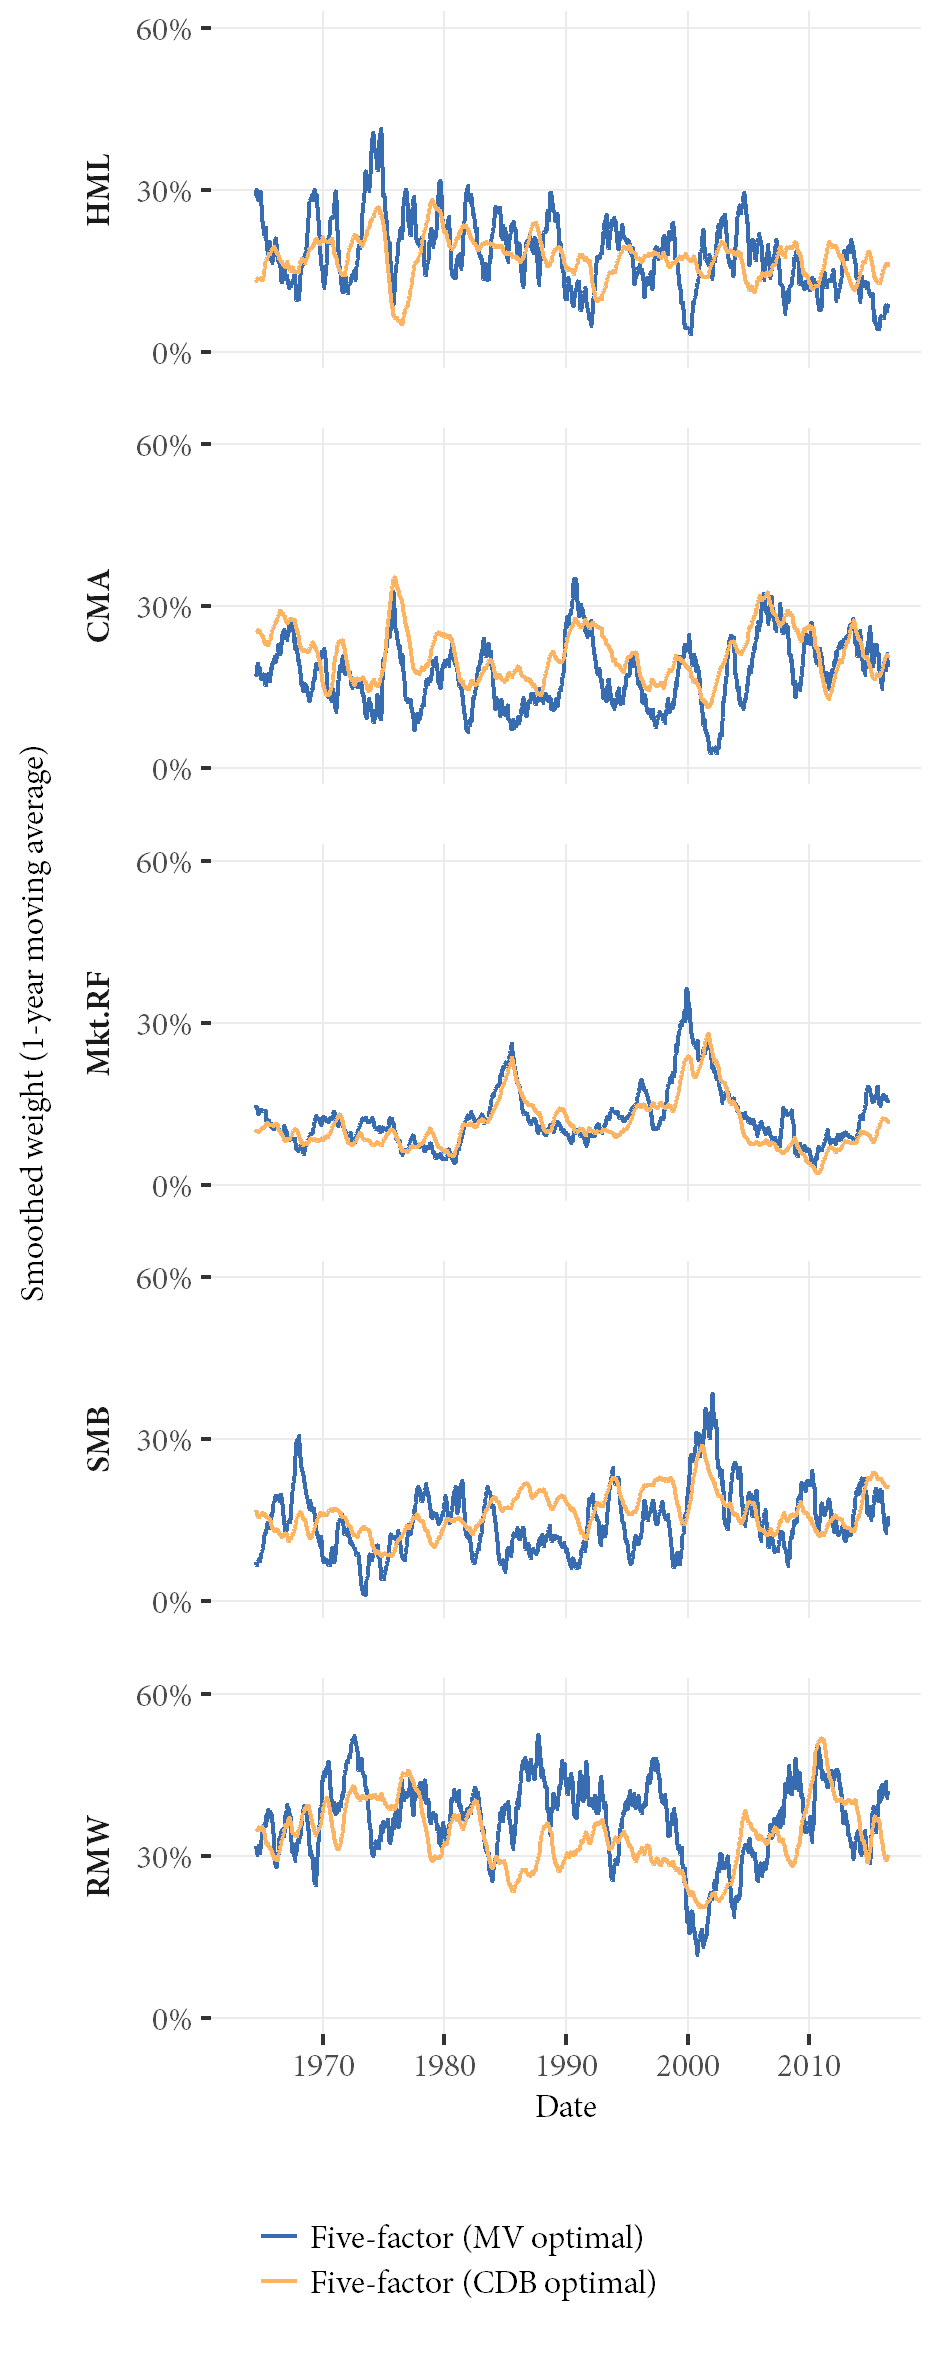
\includegraphics[width=\textwidth]{graphics/weights/compare_Weights_CDB_MV_5F.png}
    \caption{Five-factor universe}
  \end{subfigure}
  ~
  \begin{subfigure}{0.45\textwidth}
    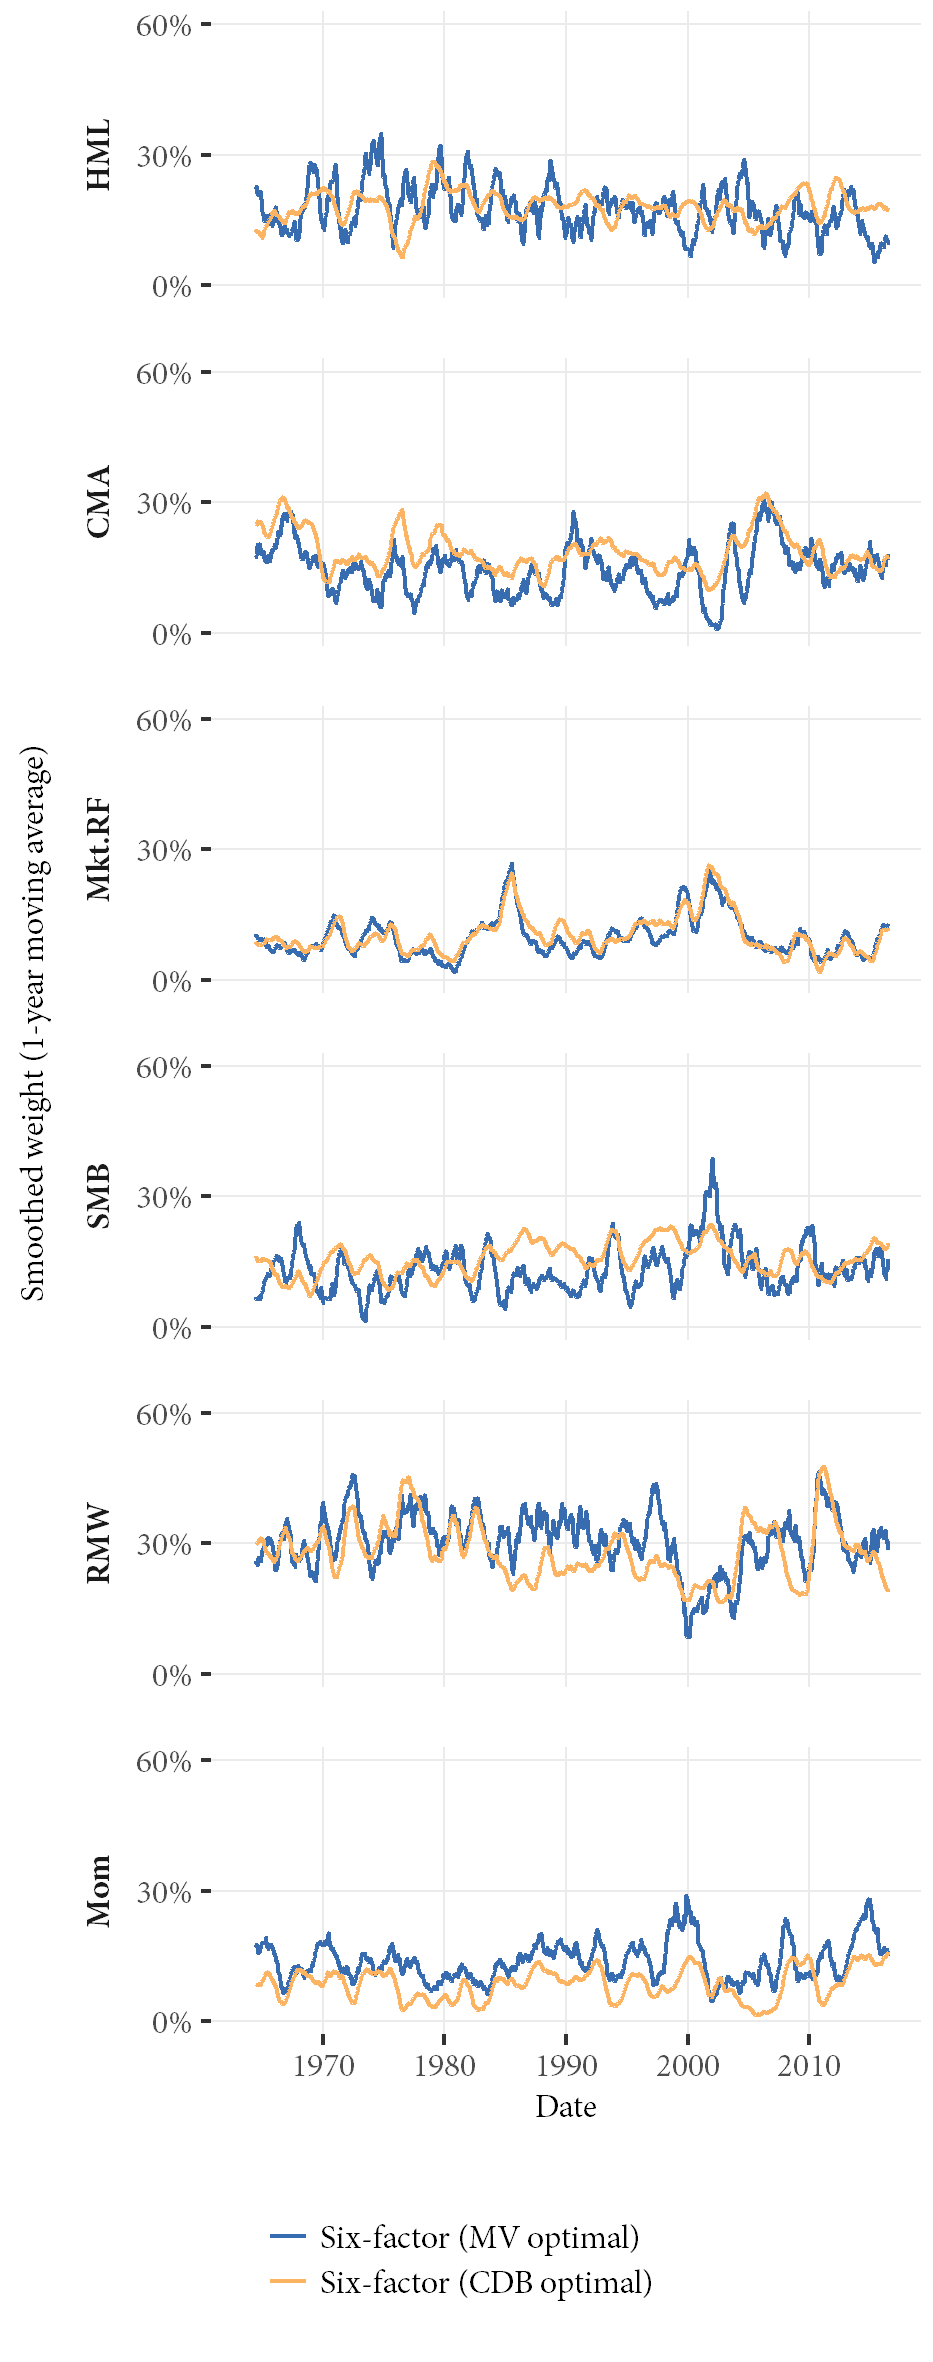
\includegraphics[width=\textwidth]{graphics/weights/compare_Weights_CDB_MV_6F.png}
    \caption{Six-factor universe}
  \end{subfigure}  
  \caption{Comparison of CDB optimal weights and MV optimal weights}
  \label{fig:cdb_mv_compare}

  \begin{longcaption}
    Smoothed as 1-year moving averages for better legibility. Optimization constrained to fully invested portfolios with non-negative weights. Based on one-week-ahead forecasts from the dynamic symmetric \emph{t} copula model 1963--2016.
  \end{longcaption}
\end{figure}

\begin{figure}[p]
  \centering
  \footnotesize
  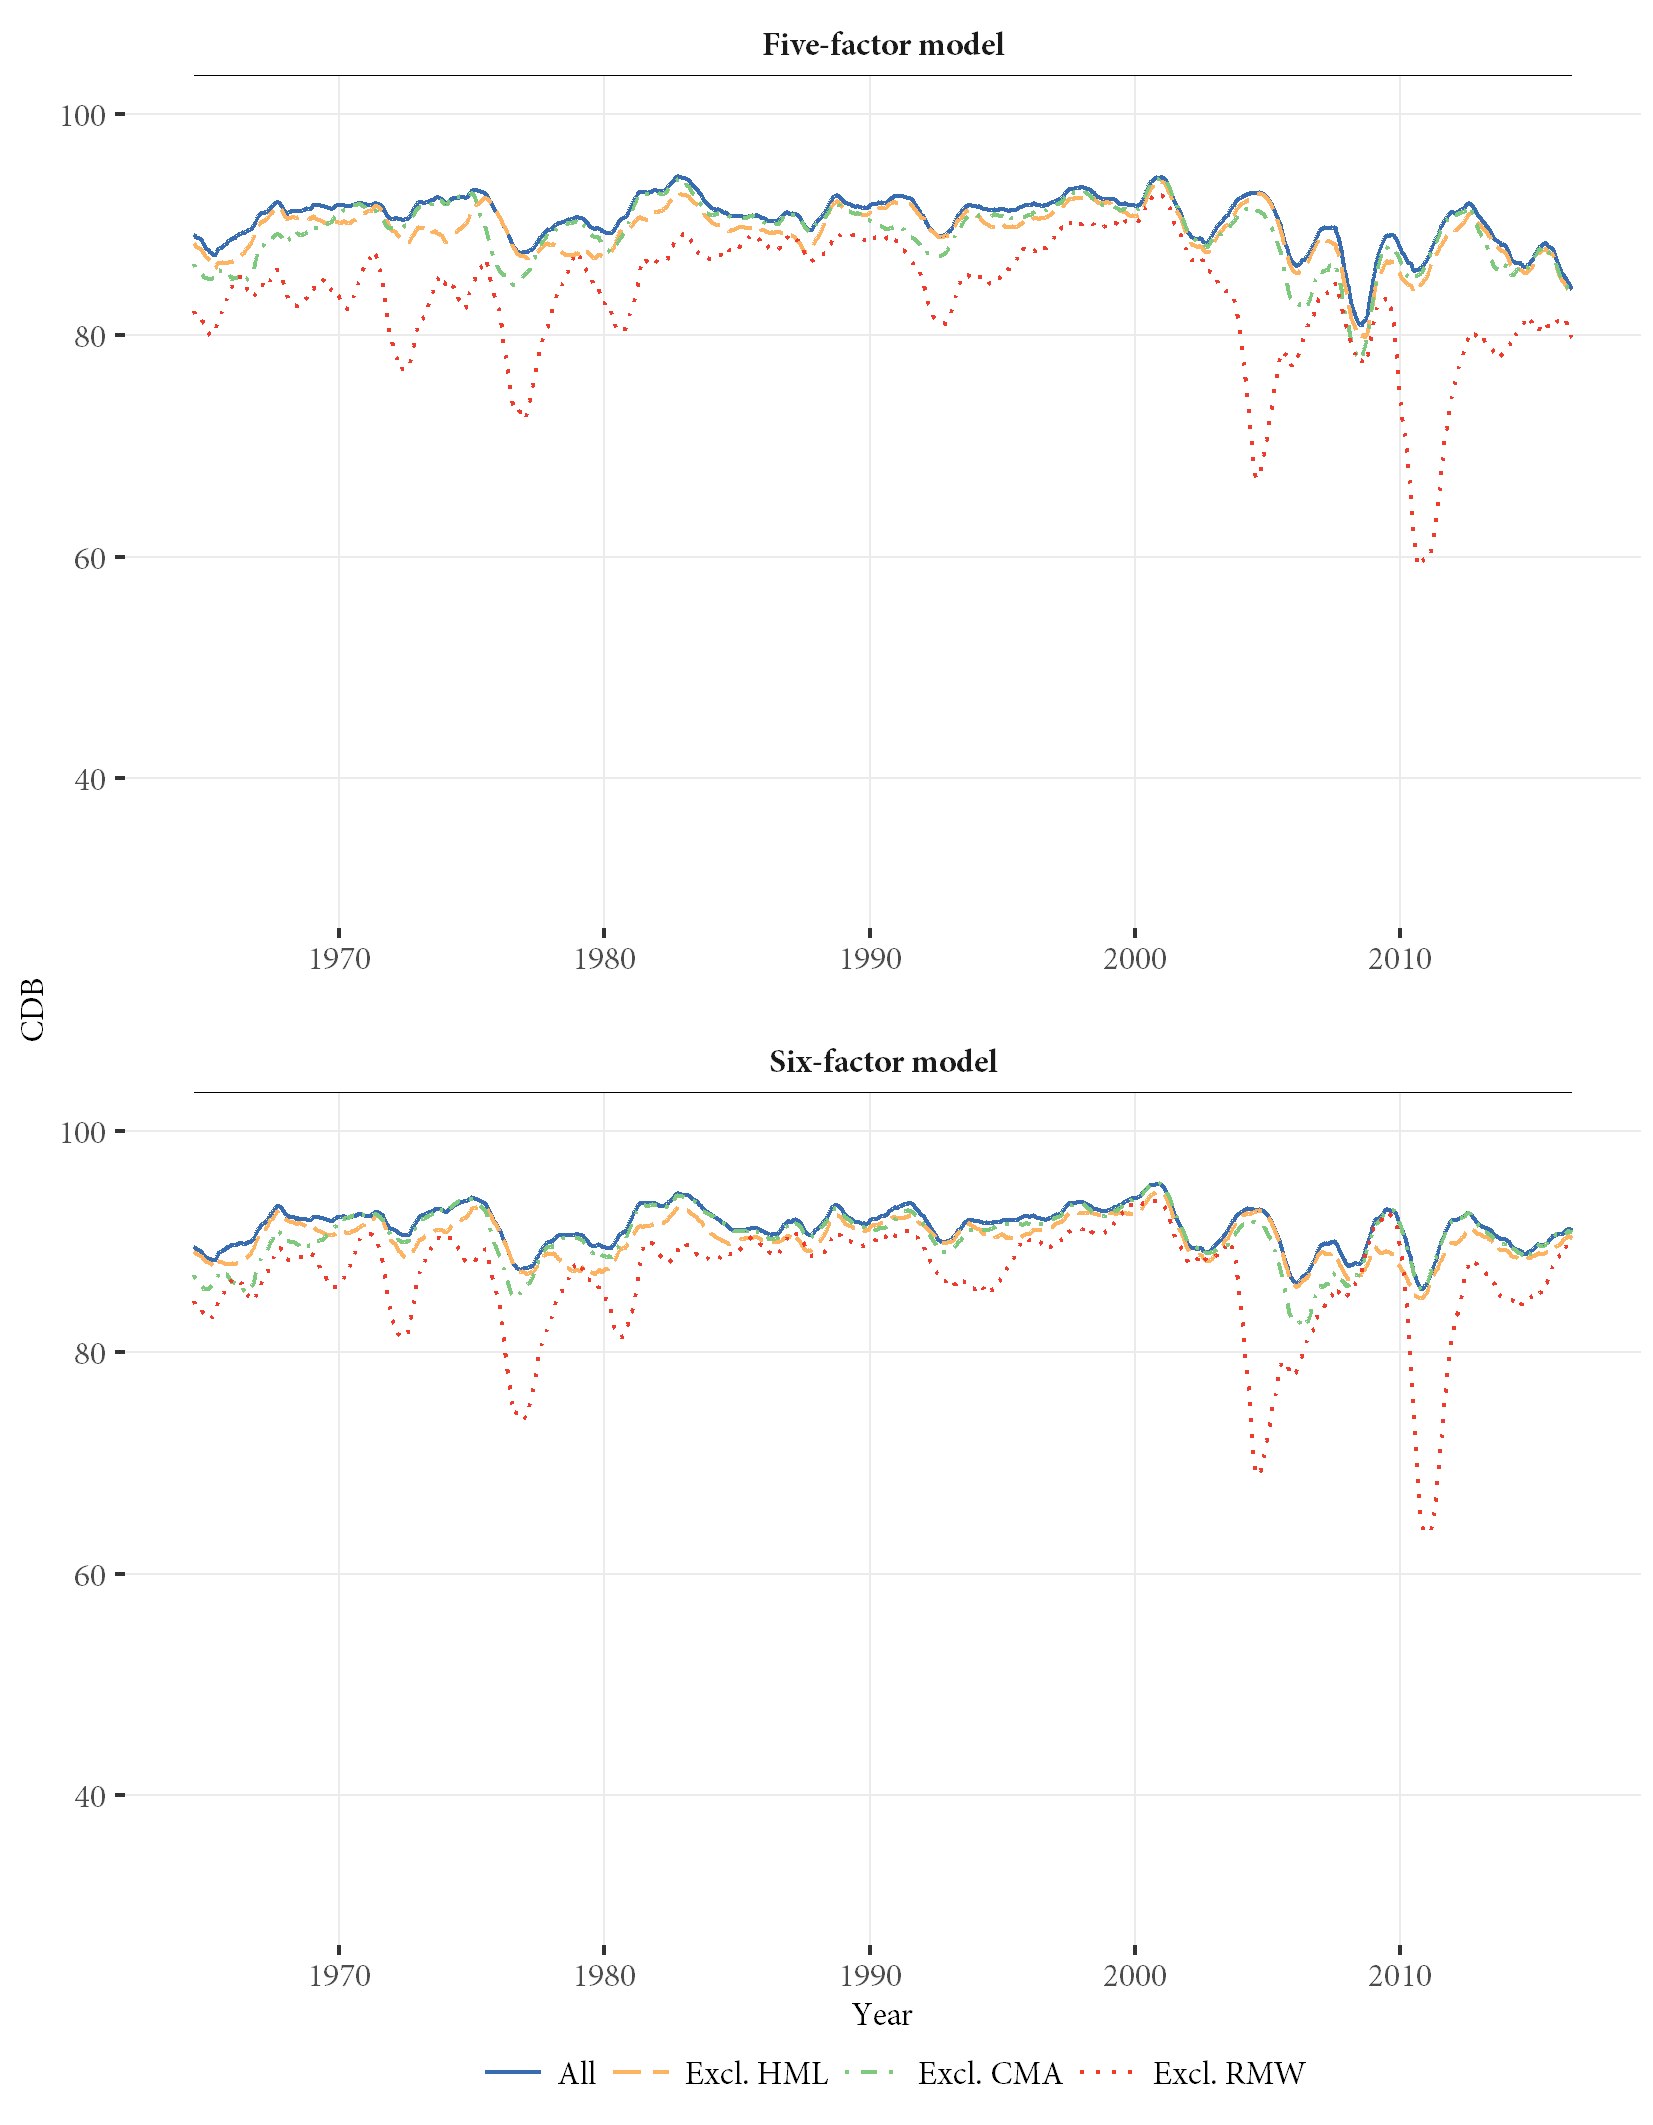
\includegraphics[width = \textwidth]{graphics/cdb/CDB.png}
  \caption{5\% Conditional Diversification Benefit (CDB) for CDB optimal weights}

  \begin{longcaption}
    Five- (without Momentum) and six-factor universes. CDB lines have been smoothed as quarterly moving averages for better legibility. See \autoref{sub:conditional_diversification_benefit} for computational details.
  \end{longcaption}
  \label{fig:cdb_cdb}
\end{figure}

\begin{figure}[p]
  \centering
  \footnotesize
  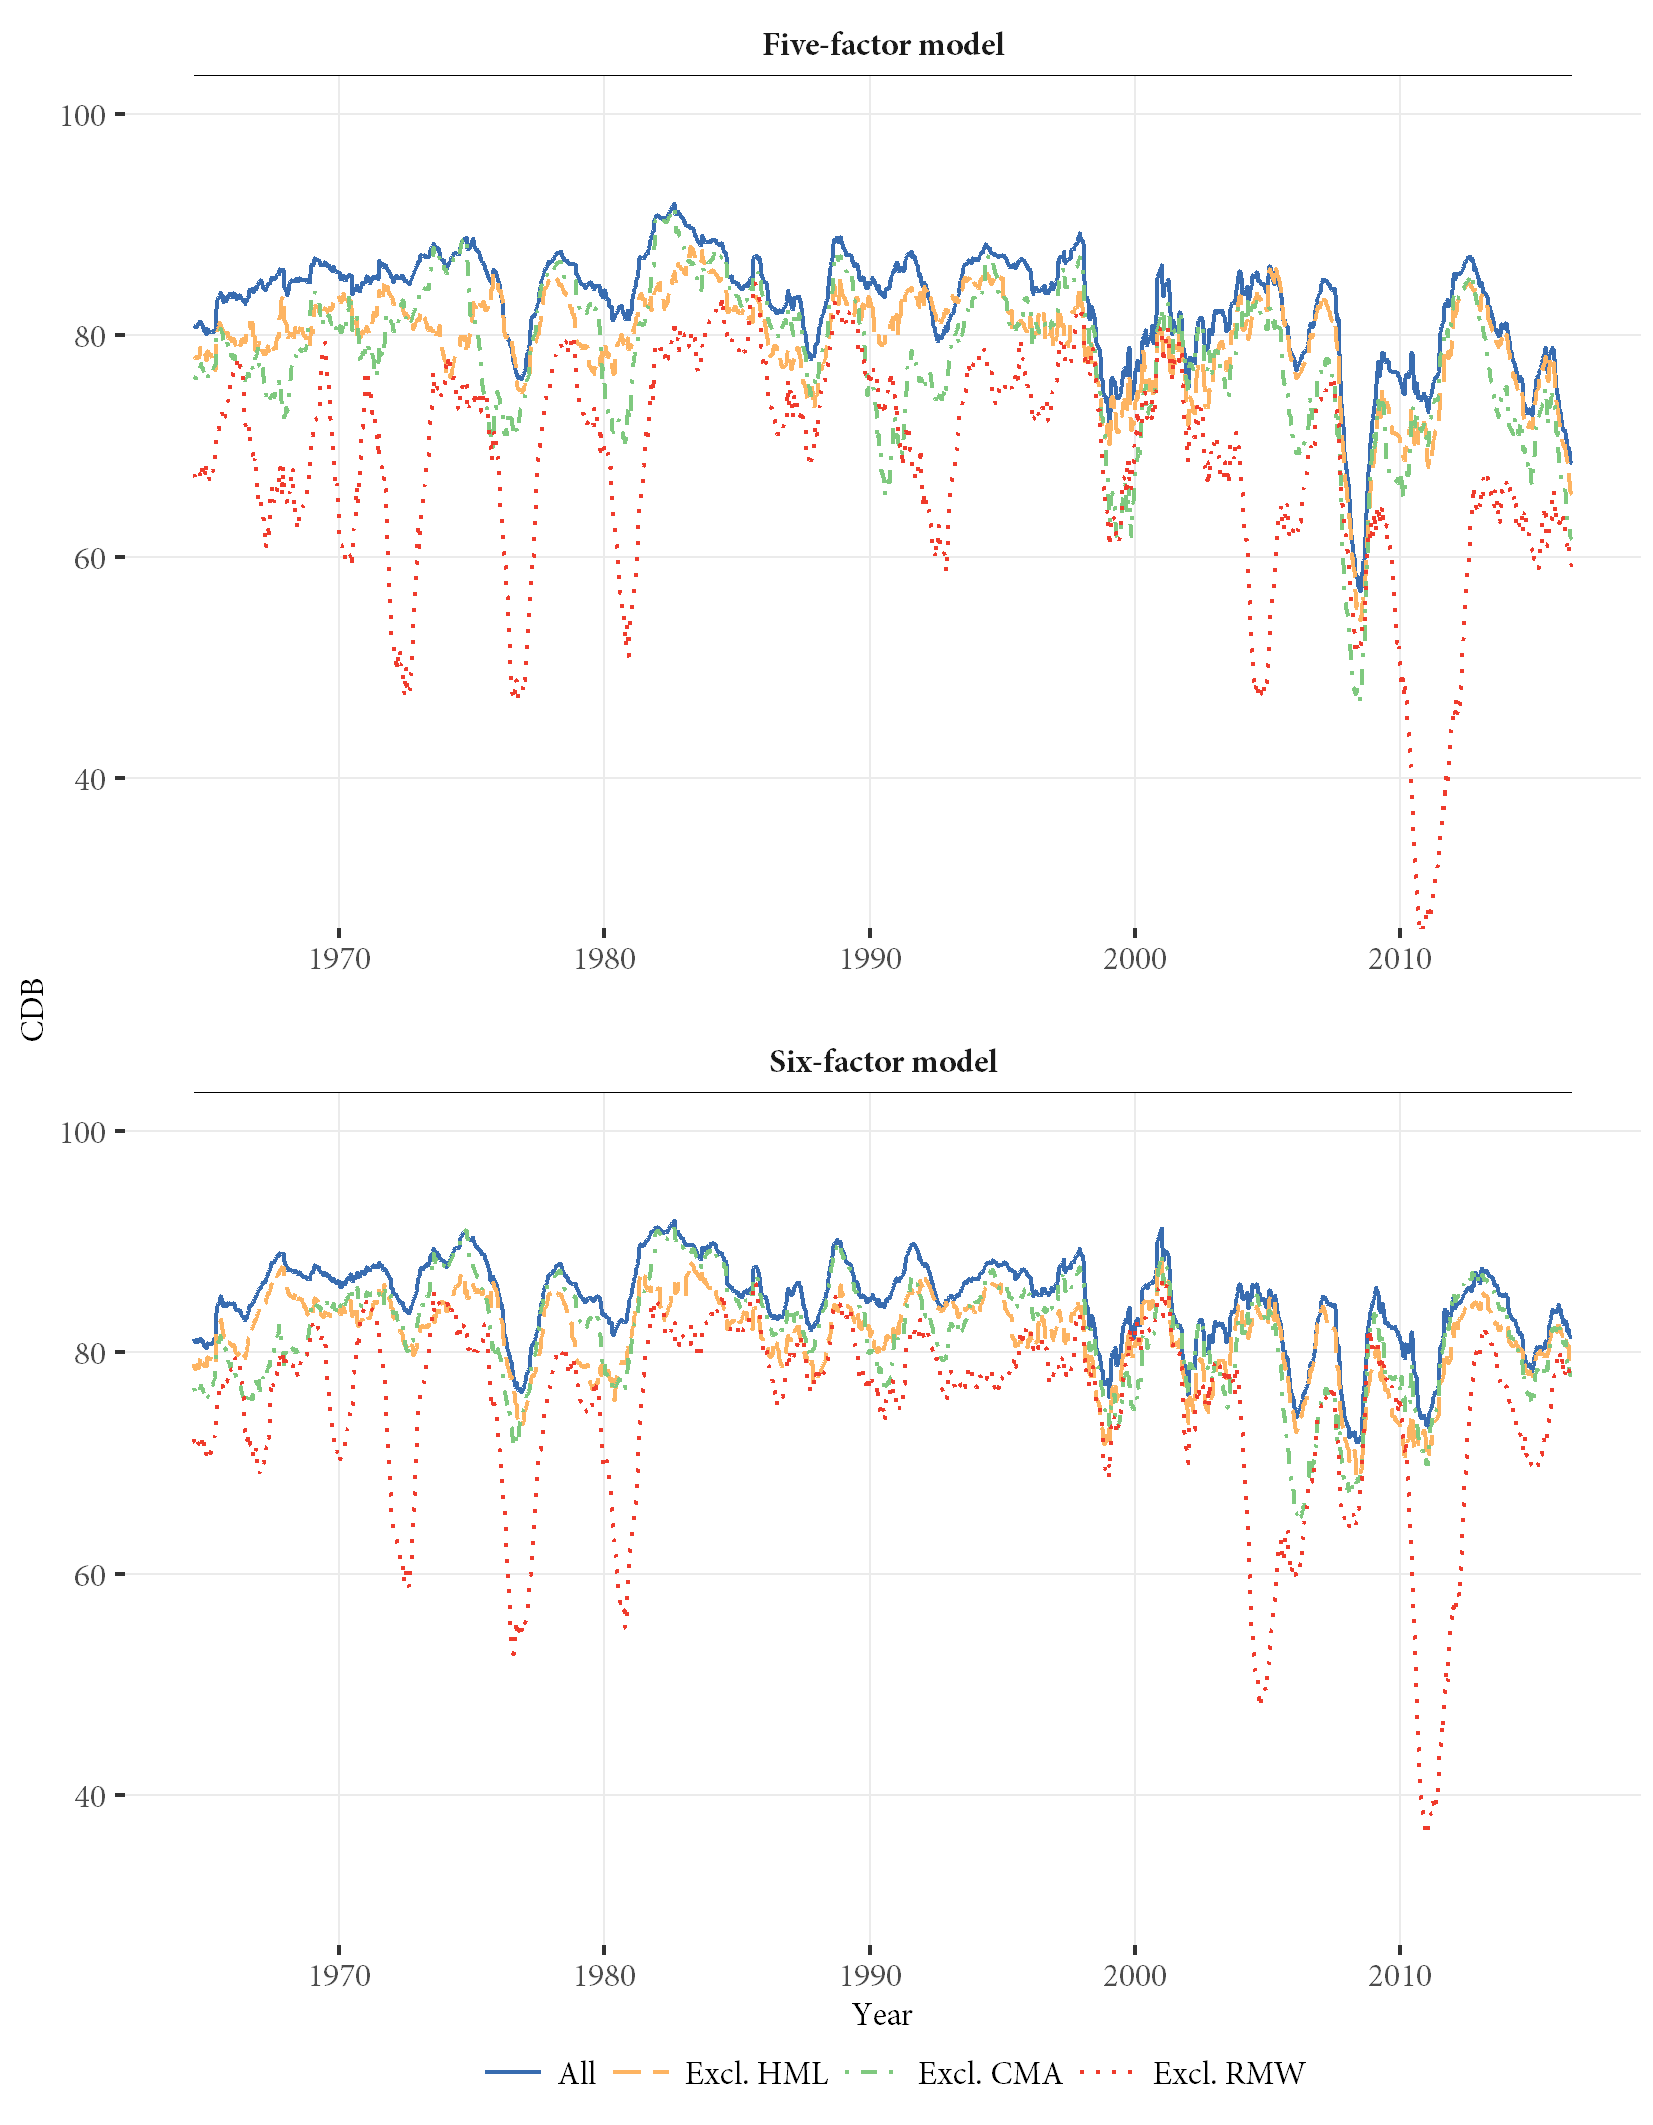
\includegraphics[width=\textwidth]{graphics/cdb/MV.png}
  \caption{5\% Conditional Diversification Benefit (CDB) for MV optimal weights}

  \begin{longcaption}
    Five- (without Momentum) and six-factor universes. CDB lines have been smoothed as quarterly moving averages for better legibility. See \autoref{sub:conditional_diversification_benefit} for computational details.
  \end{longcaption}
  \label{fig:mv_cdb}
\end{figure}

%!TEX root = ../../main.tex

\begin{table}
  \centering
  \footnotesize
  \renewcommand{\arraystretch}{1.2}

  \caption{CDB optimization with dynamic copula model (1963--2016)}

  \begin{longcaption}
    Average weights are averages of dynamic CDB optimal weights based on simulations of the return distribution from the dynamic symmetric \emph{t} copula model. Differences in average weights are expressed relative to the full five- and six-factor models. Performance measures are based on realized returns. SR is the annualized Sharpe Ratio. VaR, ES and CDB are all based on the one-week-ahead 5\% lower tail of the return distribution. Differences in CDB are to be read as column model minus row model and its associated standard errors (in parentheses) are computed taking the copula model as given.
  \end{longcaption}

  \label{tab:cdb_model}

  \begin{tabularx}{\textwidth}{@{} l dddd X dddd @{}}
    \toprule
    &
      \multicolumn{4}{c}{Five (four) factor models} &&
      \multicolumn{4}{c}{Six (five) factor models} \\
    \cmidrule{2-5}
    \cmidrule{7-10}
    &
      \multirow{2}{*}{All} &
      \multicolumn{1}{c}{Excl.} &
      \multicolumn{1}{c}{Excl.} &
      \multicolumn{1}{c}{Excl.} & &
      \multirow{2}{*}{All} &
      \multicolumn{1}{c}{Excl.} &
      \multicolumn{1}{c}{Excl.} &
      \multicolumn{1}{c}{Excl.} \\
    &
      &
      \multicolumn{1}{c}{HML} &
      \multicolumn{1}{c}{CMA} &
      \multicolumn{1}{c}{RMW} &&
      &
      \multicolumn{1}{c}{HML} &
      \multicolumn{1}{c}{CMA} &
      \multicolumn{1}{c}{RMW} \\
    \midrule
    \multicolumn{1}{@{}l}{\textbf{Average weights}} \\
    Mkt.RF & 11.1 & 10.5 & 11.5 & 19.2 & & 10.5 & 10.1  & 10.6 & 15.5 \\
    SMB    & 16.6 & 18.3 & 19.1 & 22.6 & & 15.8 & 17.9 & 18.1 & 19.2 \\
    HML    & 17.4 &      & 30.1 & 26.7 & & 18.1 &      & 28.7 & 24.9 \\
    CMA    & 21.2 & 35.0 &      & 31.6 & & 18.7 & 32.2 &      & 24.1 \\
    RMW    & 33.8 & 36.2 & 39.3 &      & & 28.1 & 31.8 & 32.6 & \\
    Mom    &      &      &      &      & &  8.8 & 8.1  & 10.0 & 16.2 \\
    \midrule
    \multicolumn{1}{@{}l}{\textbf{Difference weights}} \\
    Mkt.RF & & -0.6  & 0.4   & 8.1   & & & -0.4  & 0.2   & 5.1 \\
    SMB    & & 1.7   & 2.5   & 6.0   & & & 2.1   & 2.3   & 3.4 \\
    HML    & & -17.4 & 12.7  & 9.3   & & & -18.1 & 10.6  & 6.8 \\
    CMA    & & 13.9  & -21.2 & 10.4  & & & 13.5  & -18.7 & 5.4 \\
    RMW    & & 2.4   & 5.5   & -33.8 & & & 3.7   & 4.4   & -28.1     \\
    Mom    & &       &       &       & & & -0.7  & 1.3   & 7.5 \\
    \midrule
    \multicolumn{1}{@{}l}{\textbf{Performance}} \\
    Mean (\%)      & 2.77  & 2.94  & 2.85  & 3.37  & & 3.37  & 3.39  & 3.41  & 3.90 \\
    SD (\%)        & 2.42  & 2.49  & 2.69  & 3.89  & & 2.37  & 2.52  & 2.56  & 3.49 \\
    SR             & 1.14  & 1.18  & 1.06  & 0.87  & & 1.42  & 1.34  & 1.33  & 1.12 \\
    Avg. VaR  (\%) & 0.46  & 0.48  & 0.52  & 0.78  & & 0.45  & 0.47  & 0.49  & 0.69 \\
    Avg. ES  (\%)  & 0.61  & 0.64  & 0.69  & 1.04  & & 0.60  & 0.64  & 0.66  & 0.92 \\
    Avg. CDB       & 90.42 & 89.29 & 89.19 & 83.42 & & 91.33 & 90.24 & 90.51 & 86.62 \\
    \midrule
    \multicolumn{1}{@{}l}{\textbf{Difference CDB (column model minus row model)}} \\
    All       & & -1.13  & -1.23  & -7.01  & & & -1.09  & -0.82  & -4.71 \\
              & & (0.02) & (0.03) & (0.11) & & & (0.02) & (0.03) & (0.10) \\
    Excl. HML & &        & -0.10  & -5.88  & & &        & 0.27   & -3.62 \\
              & &        & (0.04) & (0.11) & & &        & (0.04) & (0.10) \\
    Excl. CMA & &        &        & -5.78  & & &        &        & -3.89 \\
              & &        &        & (0.11) & & &        &        & (0.10) \\
    \bottomrule
  \end{tabularx}
\end{table}


In summary, we find that the high similarity of HML and CMA indicates that tail diversification benefits are not dramatically improved by including both of the factors, which is coherent with the fact that they are closely related and overlap. However, this does not mean that both factors should not be considered jointly, as doing so could still could improve the conventional risk-return tradeoff in a mean-variance setting. The RMW factor, on the other hand, is shown to be very important for tail diversification purposes and should be considered by all factor investors concerned with tail risk.

% section cdb_optimization (end)

\pagebreak
%!TEX root = ../main.tex

\section{Discussion and conclusion} % (fold)
\label{sec:discussion_conclusion}

The first key finding of this thesis is that the classic value factor, HML, is still highly relevant for factor investors. 

Zero-cost regressions in the five-factor model suggest that HML may be fully explained by the remaining four factors, but we find evidence to the contrary. The actual implementation of mean-variance optimizations under the only constraint of non-negative weights gives a positive allocation to the HML factor. First, we have shown this using constant sample estimators as inputs in the mean-variance model on data 1963--2016. The sceptic reader will, however, object to the conclusion based on sample data alone, as a model is never better than its inputs; and sample estimates do not give a sense of optimal weights over time.

We show that, in our data, there is clear evidence of non-normality and time-variation in the dependency across factors. A mean-variance optimization that is run solely on the basis of sample estimates will ignore these features of the data, and the positive allocation to HML might be an uninteresting solution to the optimization problem.

To mitigate these concerns, we also run the mean-variance optimization using dynamic inputs from a copula model, which can generate a conditional distribution of returns that captures both the non-normality and the time-variation in dependency. Under such inputs, the allocation to HML is even greater, indicating that the classic value factor is even more attractive than sample inputs suggest.

Although variance is the staple measure of risk, we also investigate whether risk beyond the first two moments can provide reasons against the HML factor. The copula model has allowed us to infer the full distribution of returns, and we shift our focus to the tail of the distribution. Here, we find that the diversification benefit of HML is at least as great, if not greater, than that of CMA. HML can by no means be considered a worse diversifier against tail risk, as measured by expected shortfall, than CMA.

We believe that the reason why zero-cost regressions indicate that HML does not add value is that the regressions are misspecified. The omission of an important sixth factor strategy, momentum, creates a bias on all the factor loadings, and leads to not recognizing the added value of HML. While the role of HML as a unique addition was already defended by \textcite{Asness2015}, we have pursued the argument and can conclude that optimizations lead to positive allocations to the HML strategy.

Our second key finding is that HML is highly similar, but not quite the same as CMA. On a closer look, differences emerge, and we believe that factor investors should combine both factors with consideration.

There is important theoretical and empirical support for a overlap in the stock positions that comprise HML and CMA, which results in a substantially higher correlation for this factor pair than for any other factor pair. The dependence between the two factors is also more stable, and does not exhibit the same pattern of tail dependece as do other factor pairs. 

Still, one factor cannot replace the other -- they do exhibit different properties, as HML firms are more profitable and exhibit less momentum, and generate return premia that mean-variance optimization suggests combining. Beyond the risk-reward of the first two moments, analysis of the full return distribution from the copula model shows that the diversification benefit of adding either HML or CMA to a portfolio is not constant over time. Sometimes HML is the better diversifier, sometimes CMA is better, but no pattern emerges as to which factor is better than the other. We see no reason for investors to choose either one or the other, as both provide valuable diversification, and even better, they do so at different times.

However, we strongly believe that investors should consider the two factors jointly when building portfolios: When one of the two factors is included to a factor portfolio already containing the second, the first factor almost exclusively cannabilizes on the weight from the second. Our findings support the existing theoretical and empirical evidence of an overlap in the firms that comprise the two strategies. All in all, we are wary of factor weighting schemes that suggest pure equal-weights for HML and CMA. While such schemes are valuable for factor investing in general, as they avoid the pitfall of factor (mis)timing, they should be designed in a manner that takes the close link between HML and CMA into account. This pair has a very different dependence from all other pairs -- and so should also the allocation policy be different.

A third finding of this thesis is the strength of the profitability factor. The factor covaries negatively with most factors and receives zero or negative factor loadings in zero-cost regressions. The exclusion of RMW in our diversification benefit analysis completely pulls the plug on diversification, making periods of low diversification both more frequent and much more severe. Furthermore, the factor receives high allocations both using sample and model inputs in the mean-variance framework. The fact that there are no strong explanations of the profitability factor as a risk premium makes these findings even more puzzling: While investing in quality firms is by no means a new notion, there are always two investors to every trade, and the reasons for not holding profitable firms are unclear. Our takeaway is that all funds and investors in the factor space should seriously consider adding this new factor.

During the writing of this thesis, we also considered studying additional emerging factors, in particular the low volatility and betting against beta factors. At a first glance, we found highly diversifying characteristics of these factors, which remind us of RMW. It would be especially interesting to study their impact on tail risk, following the conditional diverisfication benefit analysis. We did in the end not include them as we hone in on the discussion regarding HML's role in the five- and six-factor models.

A substantial part of this thesis is built upon a rather opaque and involved copula model. While we are generally comfortable with the estimation procedure and robustness of the model, we acknowledge that it does lack the power to properly explain asymmetries in tail dependence. A natural route for an extension to a more flexible methodology would be to consider vine copulas in place of the multivariate copula we use. We also believe that the advances of regime switching models could prove fruitful in the factor setting, as such models can more rapidly adjust to shocks.

In unreported results, we have also studied out-of-sample investing with factor timing based on the copula model, but find results to be lackluster. While the copula model can ex post shed light on the roles of different factors, it is not useful for a priori portfolio allocation. This is, however, highly coherent with the preference of money managers to use static weights.\footnote{See i.a. \textcite{AQRSiren}, \textcite{BlackRock}, \textcite{MSCI} and \textcite{Robeco}.} Out-of-sample factor timing is hard, and please note that we do not purport to create a model for investment uses -- our contribution is only possible ex-post. While MV and CDB analysis based on dynamic weights may seem counter-intuitive at first, as investors use static weights, we argue that the dynamic analysis is a powerful tool for evaluation purposes.
\pagebreak
\printbibliography
\pagebreak
%!TEX root = ../main.tex
\appendix
\appendixpageoff
\section{Appendix A. Skewed Student-\textit{t} distribution} \label{App:AppendixA}
In line with stylized facts on financial return series, the factor strategies exhibit fat tails and skewness - features that are poorly represented by the normal Gaussian. Our univariate estimations as well as our copula builds on the~\textcite{Hansen1994} skewed Student-\textit{t} distribution. The skewed Student-\textit{t} distribution is, more generally, nested in the generalized hyperbolic distribution~\autocite{McNeilFreyEmbrecht2005}.

The random vector X is distributed multivariate generalized hyperbolic if
\begin{align}
    X \sim \mu + \sqrt{W} A Z + \gamma W
\end{align}
where $\mu$ is the location vector, $\gamma$ is the skewness vector, $R = A A^\top$ is the dispersion matrix, $W$ follows a generalized inverse-gamma distribution $W \sim GIG(\lambda, \chi, \psi)$ and Z is multivariate normal $Z \sim N(\mu^N, R)$, with $W, Z$ independent. The skewed Student-\textit{t} is nested with parameters
\begin{align}
    \lambda = \frac{\nu}{-2} && \chi = \nu - 2 && \psi = 0
\end{align}
where $\nu$ is the degree of freedom. Furthermore
\begin{align}
    \mathbb{E}[X] &= \mu + \mathbb{E}[W] \gamma \\
    Var[X] &= \mathbb{E}[Cov(X|W)] + Cov(\mathbb{E}[X|W]) \\
    &= Var(W) \gamma \gamma^\top + \mathbb{E}[W] R \nonumber
\end{align}
These moments describe the link between the copula correlation matrix $R$ and the skewed Student-\textit{t} distribution's dispersion matrix $R$. Covariances are finite when $\nu > 4$. The multivariate density function is given by
\begin{align} \label{eq:dskewt}
    f_X(x) &= \frac{(\nu - 2)^\frac{\nu}{2} (\gamma^\top R^{-1} \gamma)^{\frac{\nu+d}{2}}}{(2 \pi)^{\frac{d}{2}} |R|^\frac{1}{2} \Gamma (\frac{\nu}{2}) 2^{\frac{\nu}{2} - 1}} \cdot \frac{K_{\frac{\nu + d}{2}} ( \sqrt{(\nu - 2 + Q(x)) \gamma^\top R^{-1} \gamma}) e^{(x-\mu)^\top R^{-1} \gamma} )}{( \sqrt{(\nu - 2 + Q(x)) \gamma^\top R^{-1} \gamma})^{\frac{\nu + d}{2}}}
\end{align}
where $K(\cdot)$ is the modified Bessel function of the second kind, $Q(x) = (x-\mu)^\top R^{-1} (x-\mu)$, $d$ is the length of $x$, and $\Gamma$ is the gamma distribution density.

\newpage
\section{Appendix B. ARMA-GARCH modeling of marginal distributions} \label{App:AppendixB}

By examining marginal factor strategy returns (see \autoref{App:AppendixF}), we find evidence of non-normality, autocorrelation, volatility clustering and leverage effects, in line with stylized factors on financial return series (\textcite{Bollerslev1986}, \textcite{Black1976}, \textcite{glosten1993relation}). An ARMA-GARCH model allows us to filter away such marginal asymmetries, while leaving any multivariate asymmetry to the copula specification. 

The most important goal of this application GARCH model is not to have high predictive power of asset return series, but to sanitize the data to be used in multivariate analysis. We focus on parsimonious models with few lags, but enough flexibility to capture salient features of the summary plots of the marginal series, such as volatility clustering and leverage effect.

The selection process is as follows: for each factor strategy, ARMA-GJR-GARCH models are estimated with different ARMA lag orders (up to 3,3) and a fixed GJR-GARCH order of (1,1). We then compute the Bayesian Information Criterion (BIC, \textcite{Schwarz1978}) for each specification, and for each factor select the model with the lowest BIC as the primary candidate. The primary candidate specification is then checked for remaining serial correlation and ARCH effects in residuals, using the weighted portmanteau tests of \textcite{FisherGallagher2012}. All of the primary candidate models pass the diagnostic tests (see \autoref{App:AppendixE}), and additional diagnostics plots are available (see \autoref{App:AppendixG}). We use the GJR-GARCH model with ARMA mean equation
\begin{align}
    r_t &= \mu + \sum^p \phi_p r_{t-p} + \sum^q \theta_q \epsilon_{t-q} + \epsilon_{t}  \\
    \sigma_{t}^2 &= \omega + (a + \eta I_{t-1}) \epsilon_{t-1}^2 + b \sigma^2_{t-1}
\end{align}
which is estimted using maximum likelihood for each of the factor return series. The innovations $\epsilon_{i,t}$ are assumed to be distributed skewed Student-\textit{t} with skewness $\zeta$ and degree of freedom $\varrho$.

Using conditional one-step-ahead forecasts of log return and standard deviation from the ARMA-GARCH model, we can compute standardized GARCH residuals
\begin{align}
    \epsilon^*_{i,t} = \frac{\epsilon_{i,t} - E_{t-1}[\epsilon{i,t}]}{E_{t-1}[\sigma(\epsilon{i,t})]}
\end{align}
which are subsequently transformed into uniform residuals using the inverse of the skewed Student-\textit{t} distribution (\autoref{eq:dskewt}). The uniform series $\{u_i\}$ are then employed in the copula estimation.
\begin{align}
    u_{i,t} = t^{-1}_{\zeta, \varrho}(\epsilon^*_{i,t})
\end{align}

\newpage
\section{Appendix C. Stationary bootstrap of copula parameter standard errors} \label{App:AppendixC}
We rely on the multi-step maximum likelihood estimation of the copula model, which takes the standardized residuals of marginal distributions as given in the second step. The first estimation step introduces parameter uncertainty that is not taken into account by the conventional standard errors of the second estimation.\footnote{Here, our model deviates from~\textcite{ChristoffersenLanglois2013}, who use a semi-parametric model that uses the empirical density function, and find standard errors using the analytical approach in~\textcite{ChenFan2006}. However, those errors are not valid in a time-varying copula context, as the estimation of means and variances impact the asymptotic distributions of copula parameters~\autocite{Remillard2010}.} We use the stationary block bootstrap method of \textcite{PolitisRomano1994} with a block length of 45 weeks (approx. 1 year of data) to find reliable standard errors for copula parameters. The procedure is theoretically supported by \textcite{GonclavesWhite2004} and implemented as follows:
\begin{enumerate}[(i)]
    \item Generate a block bootstrap version of the original weekly return data
    \item Estimate the ARMA-GJR-GARCH models and calculate standardized residuals
    \item Transform standardized residuals to uniform and estimate the copula model
    \item Collect the copula parameters $\Theta_i$
    \item Repeat (i)-(iv) N times to get $\{\Theta_i\}^{N}_{i=1}$
    \item Use the standard errors from the empirical distribution of $\{\Theta_i\}^{N}_{i=1}$
\end{enumerate}

\newpage
\section{Appendix D. Copula correlation matrix estimation with \textit{c}DCC dynamics} \label{App:AppendixD}
This is a step-by-step description of the procedure used to find the copula correlation matrix $\{\hat{R_t}\}$ in the \textit{c}DCC case, and has been adapted from \textcite{Aielli2013}.
\begin{enumerate}[(i)]
    \item Re-standardize uniform residuals from univariate ARMA-GJR-GARCH models $\{u_{i}\}$ using the inverse skewed Student-\textit{t} distribution with copula parameters $\nu, \gamma$,  and scale to zero mean and unit variance using the conditional mean and standard deviation\footnote{Unless the copula is normal, the re-standardized residuals $\{\varepsilon^c_i\}$ will not have zero mean and unit variance, which is required for the estimation of the sample correlation matrix $\hat{S}$.}
    \begin{align}
        \varepsilon^c_{i,t} = t^{-1}_{\gamma, \nu}(u_{i,t})
    \end{align}
    \begin{align}
        \varepsilon_{i,t} = \frac{\varepsilon^c_{i, t} - E_{t-1}[\varepsilon^c_{i,t}]}{E_{t-1}[\sigma(\varepsilon^c_{i,t})]}
    \end{align}
    \item Compute the diagonal elements in $Q_t$ over time recursively, initializing with unit diagonal, and using Q-residuals $\{z_i\}$
    \begin{align}
        \intertext{Utilizing that $\S_{ii} = 1$ (for any correlation matrix), the process for diagonal elements of Q simplifies to}
        q_{ii, t} &= (1 - \alpha - \beta) + \alpha z_{t-1} z_{t-1}^\top + \beta q_{ii, t-1}
        \intertext{where residuals $\{z_{i}\}$ are initialized at zero and then calculated as}
        z_{i, t} &= \varepsilon_{i, t} \sqrt{q_{ii, t}}
    \end{align}
    \item Use Q-standardized residuals $\{z_{i}\}$ to calculate a copula sample correlation matrix
    \begin{align}
        \hat{S} = \frac{1}{T} \sum_{t=1}^{T} z_{t-1} z_{t-1}^\top
    \end{align}
    \item Calculate off-diagonal elements of the Q matrix using the copula sample correlation matrix $\hat{S}$ as the long-term correlation matrix in the \textit{c}DCC specification
    \begin{align}
        \hat{Q_t} = (1 - \alpha - \beta) \hat{S} + \alpha z_{t-1} z_{t-1}^\top + \beta Q_{t-1}
    \end{align}
    \item Standardize $\hat{Q_t}$ to the copula correlation matrix $\hat{R_t}$ (\autoref{eq:qtrtlink}) and calculate the sum of log-likelihoods for a given parameter set $\Theta = \{\nu, \gamma, \alpha, \beta\}$ (\autoref{eq:cdccllf})
\end{enumerate}
\newpage
\section{Appendix E. ARMA-GJR-GARCH estimation results}
\label{App:AppendixE}
% TABLES NEED TO BE MODIFIED IN THE FOLLOWING WAYS
% 1) Change {tabular} to {tabularx}{\textwidth} and make leftmost column an X column
%     and change top and bottom \hline to \toprule \bottomrule
%
% paste the following at start but before & \multicolumn
%
% \begin{tabularx}{\textwidth}{@{\extracolsep{5pt}} X D{.}{.}{-3} D{.}{.}{-3} D{.}{.}{-3} } 
% \\[-1.8ex] \midrule
% \\[-1.8ex] 
%
% paste the following at end after R2 row but before Note row
% \bottomrule \\[-1.8ex] 
%
% 2) Change the variable names to greeks
% 3) Change specification names if needed
% 4) Change R2 to LLH and add similar lines for Ljung-Box and ARCH-LM
% 5) Add label and caption
% 6) Paste this to get table heading description
%
% \begin{tabularx}{\textwidth}{X}
% \\[-1.8ex]\toprule
%\\[-1.8ex] 
% text goes here
% \end{tabularx}
%
% 6) Copy the whole table, only change caption, label, factor/spec labels and (1)-(3) to (4)-(6)
\begin{table}[!htbp] \centering 
  \caption{GARCH results: Mkt.RF, HML, SMB} 
  \label{tab:garch1} 
\begin{tabularx}{\textwidth}{X}
\\[-1.8ex]\toprule
\\[-1.8ex] 
\footnotesize Parameter estimates from ARMA-GJR-GARCH models. Heteroskedasticity robust standard errors in parentheses, following \textcite{White1982}. All data 1963-07-05 - 2016-07-01. Mean equation: $r_t = \mu + \sum^p \phi_p r_{t-p} + \sum^q \theta_q \epsilon_{t-q} + \epsilon_{t}$ and variance equation: $\sigma_{t}^2 = \omega + (a + \eta I_{t-1}) \epsilon_{t-1}^2 + b \sigma^2_{t-1}$. $\zeta, \varrho$ are the skewness and degree of freedom parameters of the Skewed Student-\textit{t} innovations. $\omega$ is set using variance targeting, following \textcite{EngleMezrich1995}. Ljung-Box and ARCH-LM tests are the weighted portmanteau tests with automatic lag selection from \textcite{FisherGallagher2012}.
\end{tabularx}
\begin{tabularx}{\textwidth}{@{\extracolsep{5pt}} X D{.}{.}{-3} D{.}{.}{-3} D{.}{.}{-3} } 
\\[-1.8ex]\midrule
\\[-1.8ex] 
 & \multicolumn{3}{c}{Factor series} \\ 
\cline{2-4} 
\\[-1.8ex] & \multicolumn{1}{c}{(1)} & \multicolumn{1}{c}{(2)} & \multicolumn{1}{c}{(3)}\\ 
\\[-1.8ex] & \multicolumn{1}{c}{Mkt.RF} & \multicolumn{1}{c}{HML} & \multicolumn{1}{c}{SMB}\\ 
\hline \\[-1.8ex] 
 $\mu$ & 0.001^{***} & 0.001^{**} & 0.000 \\ 
  & (0.000) & (0.000) & (0.000) \\ 
  & & & \\ 
 $\phi_1$ &  & 0.735^{***} & 0.779^{***} \\ 
  &  & (0.076) & (0.043) \\ 
  & & & \\ 
 $\theta_1$ &  & -0.621^{***} & -0.654^{***} \\ 
  &  & (0.085) & (0.055) \\ 
  & & & \\ 
 $a$ & 0.088^{***} & 0.109^{***} & 0.110^{***} \\ 
  & (0.012) & (0.002) & (0.024) \\ 
  & & & \\ 
 $b$ & 0.851^{***} & 0.872^{***} & 0.844^{***} \\ 
  & (0.004) & (0.002) & (0.036) \\ 
  & & & \\ 
 $\eta$ & 0.450^{***} & -0.047 & 0.112 \\ 
  & (0.112) & (0.057) & (0.073) \\ 
  & & & \\ 
 $\zeta$ & -2.631^{**} & 0.443 & -0.851 \\ 
  & (1.086) & (0.301) & (0.787) \\ 
  & & & \\ 
 $\varrho$ & 13.306^{***} & 9.759^{***} & 11.156^{*} \\ 
  & (3.081) & (2.160) & (6.233) \\ 
  & & & \\ 
 $\omega$ & 0.000 & 0.000 & 0.000 \\ 
\hline \\[-1.8ex] 
Observations & \multicolumn{1}{c}{2,766} & \multicolumn{1}{c}{2,766} & \multicolumn{1}{c}{2,766} \\ 
LLH & \multicolumn{1}{c}{7,052} & \multicolumn{1}{c}{8,791} & \multicolumn{1}{c}{8,571} \\ 
Variance persistence $(a+b)$ & \multicolumn{1}{c}{0.939} & \multicolumn{1}{c}{0.981} & \multicolumn{1}{c}{0.954} \\
Ljung-Box p-value & \multicolumn{1}{c}{0.111} & \multicolumn{1}{c}{0.992} & \multicolumn{1}{c}{0.631} \\ 
ARCH-LM p-value & \multicolumn{1}{c}{0.962} & \multicolumn{1}{c}{0.148} & \multicolumn{1}{c}{0.885} \\ 
\bottomrule \\[-1.8ex] 
\textit{Note:}  & \multicolumn{3}{c}{$^{*}$p$<$0.1; $^{**}$p$<$0.05; $^{***}$p$<$0.01} \\ 
\end{tabularx} 
\end{table}
% Table created by stargazer v.5.2 by Marek Hlavac, Harvard University. E-mail: hlavac at fas.harvard.edu
% Date and time: ons, okt 12, 2016 - 12:31:30
% Requires LaTeX packages: dcolumn 
\begin{table}[!htbp] \centering 
  \caption{GARCH results: Mom, RMW, CMA} 
  \label{tab:garch2} 
\begin{tabularx}{\textwidth}{X}
\\[-1.8ex]\toprule
\\[-1.8ex] 
\footnotesize Parameter estimates from ARMA-GJR-GARCH models. Heteroskedasticity robust standard errors in parentheses, following \textcite{White1982}. All data 1963-07-05 - 2016-07-01. Mean equation: $r_t = \mu + \sum^p \phi_p r_{t-p} + \sum^q \theta_q \epsilon_{t-q} + \epsilon_{t}$ and variance equation: $\sigma_{t}^2 = \omega + (a + \eta I_{t-1}) \epsilon_{t-1}^2 + b \sigma^2_{t-1}$. $\zeta, \varrho$ are the skewness and degree of freedom parameters of the Skewed Student-\textit{t} innovations. $\omega$ is set using variance targeting, following \textcite{EngleMezrich1995}. Ljung-Box and ARCH-LM tests are the weighted portmanteau tests with automatic lag selection from \textcite{FisherGallagher2012}.
\end{tabularx}
\begin{tabularx}{\textwidth}{@{\extracolsep{5pt}} X D{.}{.}{-3} D{.}{.}{-3} D{.}{.}{-3} } 
\\[-1.8ex]\midrule
\\[-1.8ex] 
 & \multicolumn{3}{c}{Factor series} \\ 
\cline{2-4} 
\\[-1.8ex] & \multicolumn{1}{c}{(4)} & \multicolumn{1}{c}{(5)} & \multicolumn{1}{c}{(6)}\\ 
\\[-1.8ex] & \multicolumn{1}{c}{Mom} & \multicolumn{1}{c}{RMW} & \multicolumn{1}{c}{CMA}\\ 
\hline \\[-1.8ex] 
 $\mu$ & 0.002^{***} & 0.001^{***} & 0.000^{**} \\ 
  & (0.000) & (0.000) & (0.000) \\ 
  & & & \\ 
 $\phi_1$ & 0.088^{***} & 0.583^{***} & 0.715^{***} \\ 
  & (0.024) & (0.192) & (0.134) \\ 
  & & & \\ 
 $\theta_1$ &  & -0.460^{**} & -0.625^{***} \\ 
  &  & (0.211)  & (0.150) \\ 
  & & & \\ 
 $a$ & 0.142^{***} & 0.076^{***} & 0.085^{***} \\ 
  & (0.005) & (0.001) & (0.004) \\ 
  & & & \\ 
 $b$ & 0.841^{***} & 0.916^{***} & 0.898^{***} \\ 
  & (0.001) & (0.000) & (0.000) \\ 
  & & & \\ 
 $\eta$ & -0.321^{***} & 0.000 & -0.156^{**} \\ 
  & (0.046) & (0.067) & (0.069) \\ 
  & & & \\ 
 $\zeta$ & -2.420 & 0.108 & 0.262 \\ 
  & (3.180) & (0.298) & (0.329) \\ 
  & & & \\ 
 $\varrho$ & 12.969 & 10.383^{***} & 10.148^{***} \\ 
  & (11.139) & (3.656) & (2.447) \\ 
  & & & \\ 
 $\omega$ & 0.000 & 0.000 & 0.000 \\ 
\hline \\[-1.8ex] 
Observations & \multicolumn{1}{c}{2,766} & \multicolumn{1}{c}{2,766} & \multicolumn{1}{c}{2,766} \\ 
LLH & \multicolumn{1}{c}{7,972} & \multicolumn{1}{c}{9,874} & \multicolumn{1}{c}{9,585} \\
Variance persistence $(a+b)$ & \multicolumn{1}{c}{0.983} & \multicolumn{1}{c}{0.992} & \multicolumn{1}{c}{0.983} \\
Ljung-Box p-value & \multicolumn{1}{c}{0.065} & \multicolumn{1}{c}{0.062} & \multicolumn{1}{c}{0.634} \\ 
ARCH-LM p-value & \multicolumn{1}{c}{0.051} & \multicolumn{1}{c}{0.912} & \multicolumn{1}{c}{0.926} \\  
\bottomrule \\[-1.8ex] 
\textit{Note:}  & \multicolumn{3}{c}{$^{*}$p$<$0.1; $^{**}$p$<$0.05; $^{***}$p$<$0.01} \\ 
\end{tabularx} 
\end{table}
\newpage
\section{Appendix F. Marginal series inspection}
\label{App:AppendixF}
\newpage
\section{Appendix G. GARCH model diagnostics}
\label{App:AppendixG}
\end{document}
